\documentclass[journal]{IEEEtran}

\usepackage{amsmath,amssymb,amsthm,mathtools}
\usepackage{graphicx}
\usepackage{booktabs,array}
\usepackage{cite}
\usepackage{microtype}
\usepackage[hidelinks]{hyperref}
\usepackage{url}

\interdisplaylinepenalty=2500
\setlength{\emergencystretch}{1.5em}

\newtheorem{theorem}{Theorem}
\newtheorem{lemma}[theorem]{Lemma}
\newtheorem{appendixlemma}[theorem]{Lemma}
\newtheorem{proposition}[theorem]{Proposition}
\newtheorem{corollary}[theorem]{Corollary}
\newtheorem{conjecture}[theorem]{Conjecture}
\theoremstyle{definition}
\newtheorem{definition}[theorem]{Definition}
\theoremstyle{remark}
\newtheorem{remark}[theorem]{Remark}

% Compatibility wrappers for explanatory remarks retained in technical appendices.
\newenvironment{intuition}[1]{\begin{remark}[#1]}{\end{remark}}
\newenvironment{notebox}{\begin{remark}}{\end{remark}}

\newcommand{\E}{\mathbb E}
\newcommand{\Ent}{\operatorname{Ent}}
\newcommand{\Inf}{\operatorname{Inf}}
\newcommand{\atanh}{\operatorname{atanh}}
\newcommand{\sech}{\operatorname{sech}}
\newcommand{\Fhat}[1]{\widehat{#1}}
\newcommand{\R}{\mathbb R}
\newcommand{\Q}{\mathbb Q}
\newcommand{\diff}{\,\mathrm d}
\newcommand{\Lapl}{\mathcal L}
\newcommand{\degree}{d}
\newcommand{\logodds}{\ell_\rho}
\newcommand{\weight}{\omega}
\newcommand{\Klsi}{K_{\mathrm{LS}}}
\newcommand{\cutoff}{v_{\mathrm{cut}}}
\newcommand{\edgewidth}{d_{\mathrm{edge}}}
\newcommand{\corr}{\operatorname{corr}}
\newcommand{\unitcost}{\operatorname{yield}}

\hypersetup{
  pdftitle={The Most Informative Bit: A Proof of the Courtade--Kumar Conjecture and Multibit Extensions},
  pdfauthor={Ahmad Beirami and Hessam Mahdavifar},
  pdfsubject={Boolean functions, noisy channels, and multibit quantization}
}


\begin{document}

\title{The Most Informative Bit and Beyond: \\A Proof of the Courtade--Kumar Conjecture \\and Multibit Extensions}

\author{Hessam~Mahdavifar and Ahmad~Beirami
\thanks{H. Mahdavifar is with the Department of Electrical and Computer
Engineering, Northeastern University, Boston, MA 02115 USA
(e-mail: h.mahdavifar@northeastern.edu).}
\thanks{A. Beirami is with Fidian, San Francisco,
CA, USA (e-mail: ab@fidian.ai).}%
}

\maketitle


\begin{abstract}
Let \(X=(X_1,\ldots,X_n)\) be uniform on the Boolean cube, and let \(Y\)
be obtained by passing its coordinates independently through a binary
symmetric channel with crossover probability \(p\). A natural quantization
question asks how much information about \(Y\) can be retained by a
function \(Q(X)\) constrained to \(k\) output bits. For \(k\leq n\),
reporting \(k\) input coordinates retains \(k(1-h_2(p))\) bits of
information, where \(h_2\) denotes the binary entropy function. This
makes coordinate projections the natural benchmark.

The case \(k=1\) is the Courtade--Kumar conjecture, which posits that every
Boolean function \(f\) satisfies
\[
    I(f(X);Y)\leq 1-h_2(p),
\]
with equality attained by coordinate functions. We prove this conjecture
for every dimension and crossover probability, without any balance
assumption on \(f\). Our proof views the gap relative to the coordinate
benchmark as a quantity that evolves with the channel correlation. After
a monotone rearrangement, an entropy-flow identity relates its derivative
to the edge boundary of the corresponding Boolean decision set. Combining
a sharp local entropy comparison with Fourier analysis on the Boolean cube
and logarithmic Sobolev estimates for pivotal sets yields a global
differential inequality: if the gap is positive at any correlation level,
then it must grow as the noise decreases. This contradicts the noiseless
endpoint, where the gap is nonpositive.

For \(k\geq8\), however, a distinctly coding-theoretic behavior emerges.
We construct quantizers from shortened Hamming codes whose covering
structure beats the coordinate-projection benchmark for \(k=8\), and a
direct-sum argument extends this failure to every \(k\geq8\). Thus, unlike
in the single-bit case, structured coding can retain more information than
simple coordinate selection. Finally, exhaustive searches within several
structured code families and Monte Carlo searches over random codebooks
for \(2\leq k\leq7\) reveal a clear advantage of structured codebooks over
random ones while still underperforming the coordinate benchmark. These findings
lead us to conjecture that coordinate projections remain optimal for
\(2\leq k\leq7\).
\end{abstract}

\begin{IEEEkeywords}
Binary symmetric channel, Boolean functions, Courtade--Kumar conjecture,
Fourier analysis, Hamming codes, logarithmic Sobolev inequality, mutual
information, quantization.
\end{IEEEkeywords}

\section{Introduction}
\label{sec:introduction}

Let \(X=(X_1,\ldots,X_n)\) be a sequence of independent uniform binary
random variables, and let \(Y\) be obtained by passing every coordinate
through a binary symmetric channel (BSC) with crossover probability
\(p\in[0,1/2]\). A Boolean summary \(f(X)\) retains one bit from the
input. Courtade and Kumar conjectured that the mutual information between
this summary and the complete noisy observation is maximized by retaining
one of the original coordinates~\cite{CK}. Equivalently,
\begin{equation}
 I(f(X);Y)\leq 1-h_2(p),
 \label{eq:intro-ck}
\end{equation}
where \(h_2\) is the binary entropy function. Equality is attained by any
\textit{dictator} defined as \(f(X)=X_i\) for some \(i \in \{1,2,\dots,n\}\).

The problem is different from maximizing correlation or noise
stability. The observation \(Y\) is an \(n\)-dimensional random vector,
and information carried jointly by its coordinates need not decompose
into coordinatewise contributions. For example, the parity of two noisy
bits can contain information that is absent from either noisy bit alone.
Consequently, results for two Boolean outputs~\cite{AGKN,PPM} or for sums
of coordinatewise mutual informations~\cite{JW} do not directly imply
\eqref{eq:intro-ck}. The output \(f(X)\) may also be biased, which removes
several symmetries available in the balanced case.

This paper establishes \eqref{eq:intro-ck} in full generality. The proof
uses the correlation parameter \(\rho=1-2p\). After monotone sorting, the
mutual information becomes an entropy functional of the posterior mean
\(T_\rho f\). Its derivative admits an edge decomposition. The central
step is to strengthen the entropy-constrained edge envelope by retaining
the squared angular displacement lost in a Cauchy--Schwarz comparison.
The pivotal sets of the same Boolean function supply the Fourier and
logarithmic-Sobolev control needed to pay for this correction. The final
argument is dynamical: wherever a function has more information than a
dictator, its advantage must increase with \(\rho\). Such an advantage
cannot return to its nonpositive value at \(\rho=1\).

We also study the natural vector-valued extension in which \(f(X)\)
contains \(k\) bits. The scalar theorem does not tensorize through the
chain rule because conditioning on preceding output bits destroys the
uniform input law. In fact, the coordinate benchmark is false for
sufficiently large fixed \(k\). We give explicit shortened-Hamming
counterexamples for \(k=8,9,10\), extend them to every \(k\geq8\), and
formulate a threshold conjecture for \(2\leq k\leq7\).

\subsection{Related Work}

Courtade and Kumar introduced the full-vector problem and proved several
structural reductions, including the monotone sorting operation used
below~\cite{CK}. The conjecture stimulated a sequence of Fourier,
functional-inequality, and information-geometric approaches. The
Friedgut--Kalai--Naor theorem identifies the rigidity of Boolean functions
whose Fourier mass is concentrated on the first two levels~\cite{FKN}.
Samorodnitsky established the conjecture in a dimension-free high-noise
regime and developed strengthened inequalities for the entropy of noisy
Boolean functions~\cite{Sam,SamEntropy}. Ordentlich, Shayevitz, and
Weinstein obtained sharper balanced high-noise bounds using Fourier
analysis and hypercontractivity~\cite{OSW}, while Yang and Wesel gave a
complementary calculus argument in a dimension-dependent neighborhood of
complete noise~\cite{YW}.

Yu developed a general \(\Phi\)-stability framework and subsequently
proved broad local-optimality and balanced finite-range results using
quantitative Fourier estimates~\cite{YuPhi,Yu,YuSharp}. Javanmard and
Woodruff proved the dictator bound for the sum of the individual-coordinate
mutual informations and sharpened the high-noise analysis~\cite{JW}; the
related Boolean-hull and moment relaxations are discussed in~\cite{Gemini}.
Li and M\'edard connected the problem to posterior moments and
noninteractive correlation distillation~\cite{LM}, and Barnes and
\"Ozg\"ur showed that the balanced conjecture is essentially equivalent
to a symmetrized Li--M\'edard formulation~\cite{BO}.

A second line of work seeks stronger entropy or isoperimetric statements.
Anantharam, Bogdanov, Chakrabarti, Jayram, and Nair proposed a Hellinger
inequality implying the conjecture~\cite{Hellinger}. Chen and Nair placed
this proposal in an ordered family of entropy inequalities and related
the low-noise limits to sharp cube isoperimetry~\cite{CN}. The critical
square-root isoperimetric inequality was recently established by Durcik,
Ivanisvili, Roos, and Xie~\cite{DIRX}. These limiting or stronger
statements do not themselves yield the finite-noise Shannon inequality.

The closest antecedent to the present proof is the differential-equation
framework odf Chen, Gohari, and Nair~\cite{CGN}. Their entropy-flow identity
and entropy-constrained two-point extremal formula are used here. 

Two
concurrent works establish the scalar conjecture in full
generality~\cite{CGJLMNW,KyTran}. Chen, Gohari, Javanmard, Lin, Mirrokni,
Nair, and Woodruff close the differential-equation program through an
unrestricted four-moment Bellman inequality for a hybrid potential,
using analytic reductions together with certified interval arithmetic.
Ky and Tran instead develop an entropy-production and spectral framework.
Their method is substantially closer to ours: both arguments use monotone
compression, edgewise entropy-production estimates, Fourier control of
functions with diffuse coordinate dependence, separate channel regimes,
and a differential contradiction at the noiseless endpoint. The
quantitative implementations differ. Our proof centers on an angular
edge correction and logarithmic-Sobolev estimates for pivotal sets,
whereas Ky and Tran use a profile-clock integration and selected-coordinate
spectral estimates. Finally, neither of~\cite{CGJLMNW,KyTran} considers the \(k\)-bit extension
studied in the present paper where we conjecture that up to $k=7,$ the most informative \(k\)-bit function follows a similar structure.

Related operator and channel perspectives include principal inertia
components~\cite{PIC} and mutual-information bounds based on adjacency
events~\cite{HOS}. Continuous analogues and stochastic-interpolation
variants were developed in~\cite{KOW,EMR}.

The present paper additionally develops the vector-valued extension in
which the quantizer reports \(k\) bits. For this problem, Chandar and
Tchamkerten characterized the positive-rate asymptotics and
gave Hamming- and Golay-code counterexamples with \(k\geq11\)~\cite{CT}.
Huleihel and Ordentlich proved coordinate optimality at the complementary
endpoint \(k=n-1\)~\cite{HO}. The finite-block behavior observed in our
code search is also related qualitatively to recent results showing that
structured Reed--Solomon-based codebooks can outperform random codebooks
under average Hamming covering radius~\cite{RMcover}; the objective in
that work is different from BSC mutual information.

\subsection{Contributions and Organization}

Our fist main contribution is Theorem~\ref{thm:CK}, which proves the
Courtade--Kumar conjecture in every dimension and for every crossover
probability, without any balance assumption on the Boolean function. The
proof follows a single dynamical strategy. For
$
 I_f(\rho)\coloneqq I(f(X);Y_\rho),
 \phi(\rho)\coloneqq I(X_1;Y_\rho),
 \Delta_f(\rho)\coloneqq I_f(\rho)-\phi(\rho),
$
we show that a positive advantage over a coordinate projection would have
to grow strictly as the channel becomes less noisy. Section~\ref{sec:mechanism}
introduces the posterior representation of \(I_f\), the required Fourier
notation, and the monotone reduction. In particular,
Lemma~\ref{lem:sorting} shows that coordinatewise sorting preserves any
advantage, allowing the remainder of the proof to exploit the
edge structure of a monotone Boolean decision set. An entropy-flow
identity expresses \(\rho I_f'(\rho)\) as an action functional of the
posterior mean \(T_\rho f\). Section~\ref{sec:edges} then decomposes this
action over edges of the discrete cube. The key estimate,
Lemma~\ref{lem:edges}, strengthens the usual two-point entropy envelope by
retaining a squared angular correction that is exact for dictators. The
rest of the proof shows that the Boolean and spectral structure of \(f\)
always provides enough reserve to pay for this correction.

Writing \(\ell=\operatorname{arctanh}\rho\), we divide the channel into
the small-correlation range \(0\leq\ell\leq31/20\), the intermediate
range \(31/20\leq\ell\leq7/2\), and the near-noiseless tail
\(\ell\geq7/2\). Equivalently, the two junctions are
\(\rho=\tanh(31/20)\) and \(\rho=\tanh(7/2)\). These cutoffs are technical
junctions at which the corresponding estimates meet, rather than
asserted phase transitions in the problem. Proposition~\ref{prop:low}
settles the small-correlation range directly, at every output bias, by
combining a Fourier energy gap with scalar entropy bounds. In the
intermediate range, the pivotal sets of \(f\) supply the needed reserve:
logarithmic Sobolev inequalities control the noisy entropies of their
indicators, and a log-sum argument combines the coordinatewise costs with
the global edge budget. This yields
Proposition~\ref{prop:middle-growth}, according to which
\(\Delta_f(\rho)>0\) implies \(\Delta_f'(\rho)>0\) throughout that range.
The bounded angular reserve is insufficient by itself near the noiseless
endpoint, so the tail argument supplements the same edgewise inequality
with degree-weighted Fourier information. Lemma~\ref{lem:deficit}
identifies the relevant coordinate deficits,
Lemma~\ref{lem:baseline} converts the information advantage into an
entropy-funded spectral baseline, and Lemma~\ref{lem:budget} turns the
resulting budget comparison into strict information growth.
Proposition~\ref{prop:local} separately rules out a counterexample having
a sufficiently influential coordinate. Section~\ref{sec:coverage}
assembles these complementary estimates in
Lemma~\ref{lem:coverage}, which gives the global implication
\[
 \Delta_f(\rho)>0\quad\Longrightarrow\quad\Delta_f'(\rho)>0.
\]
Since \(\Delta_f(1)=H(f(X))-\log 2\leq0\), a positive advantage cannot
persist to the noiseless endpoint; this contradiction completes the proof
of Theorem~\ref{thm:CK}.

Our second contribution, developed in
Section~\ref{sec:multibit-extension}, concerns the natural extension in
which the quantizer reports \(k\) bits and the coordinate benchmark is
\(k(1-h_2(p))\). Proposition~\ref{prop:affine-multibit} shows that affine
linear maps cannot violate this benchmark. Nonlinear nearest-codeword
quantizers built from linear codebooks behave differently: an exact
high-noise expansion, expressed through the coset-leader distribution,
produces shortened-Hamming counterexamples for \(k=8,9,10\) in
Proposition~\ref{prop:k8-k10-counterexamples}. A direct-sum construction
in Proposition~\ref{cor:failure-all-k-ge-8} extends the failure to every
\(k\geq8\). For \(k<8\), exhaustive searches over several structured
code families and Monte Carlo experiments with random codebooks find no
violation, while also showing a clear advantage of structured codebooks
over random ones in this finite-block regime. These findings motivate
Conjecture~\ref{conj:seven-bit-threshold}, which predicts that coordinate
projections remain optimal for \(2\leq k\leq7\). The appendices provide
the scalar inequalities, logarithmic-Sobolev and Fourier estimates,
channel-range comparisons, endpoint reductions, exact arithmetic
certificates, and reproducible numerical diagnostics used throughout the
proof.


\section{Problem Formulation and Preliminaries}
\label{sec:mechanism}

\subsection{Posterior-Mean Representation}

Let \(n\) be a positive integer, \(X\) a uniform sign string in
\(\{-1,1\}^n\), and \(f\) a function from these strings to \(\{-1,1\}\).
Obtain \(Y\) by flipping
each bit with probability \((1-\rho)/2\). Correlation \(\rho=0\)
means complete noise; \(\rho=1\) means no noise. Define
\begin{align*}
 L&=\log2,\qquad h(r)=L-\phi(r),\\
 \phi(r)&=\frac{1+r}{2}\log(1+r)
          +\frac{1-r}{2}\log(1-r).
\end{align*}
Thus \(h(r)\) is the entropy of a sign-valued bit whose mean is \(r\).
In particular, \(h(0)=L\), \(h(\pm1)=0\), and
\(\phi'(r)=g(r):=\atanh r\).

For \(m=\E f\), write
\[
u(y)=T_\rho f(y)=\E[f(X)\mid Y=y].
\]
Constant rules retain no information, so only nonconstant \(f\) need
be studied. For these, \(-1<u(y)<1\) when \(0<\rho<1\), since
every input string has positive conditional probability.
The conditional probabilities of \(f(X)\) are \((1+u(y))/2\) and
\((1-u(y))/2\). The mutual information is therefore
\begin{equation}
 I_f(\rho)=h(m)-\E h(u)=\E\phi(u)-\phi(m).
 \label{eq:posterior-information}
\end{equation}
Every expectation without a subscript is uniform on the appropriate cube.
All logarithms are natural, so information is measured in nats.
This is the full-vector objective of Courtade and Kumar~\cite{CK}.
It differs from the two-Boolean-output objective settled in~\cite{PPM}
and the sum of coordinate informations bounded in~\cite{JW,Gemini}:
the conditional expectation above retains the entire observation \(Y\).

\begin{remark}[Dictator normalization]
If \(f(x)=x_1\), then \(m=0\), \(u(y)=\rho y_1\), and
\[
 I_f(\rho)=L-h(\rho)=\phi(\rho).
\]
The target is \(I_f(\rho)\le\phi(\rho)\). The parameter \(\rho\) is the
correlation, not the crossover probability.
\end{remark}

\begin{theorem}[Courtade--Kumar inequality]
\label{thm:CK}
For every positive integer \(n\), every Boolean function
\(f:\{-1,1\}^n\to\{-1,1\}\), and every \(0\leq\rho\leq1\),
\begin{equation}
 I(f(X);Y)\leq\phi(\rho).
 \label{eq:main-ck-sign}
\end{equation}
\end{theorem}

\subsection{Boolean Fourier Representation and Entropy Flow}

Write \([n]=\{1,\ldots,n\}\). For a subset \(S\subseteq[n]\), its
size is \(|S|\); the empty subset is \(\varnothing\).
Define \(\chi_S(x)=\prod_{i\in S}x_i\), with empty product one.
The Fourier coefficient of any cube function \(v\) is
\(\widehat v(S)=\E[v(X)\chi_S(X)]\).
The parity functions form an orthonormal
basis under the uniform measure. Thus
\[
 f=\sum_{S\subseteq[n]}\widehat f(S)\chi_S,\qquad
 \E f^2=\sum_S\widehat f(S)^2.
\]
A degree-\(|S|\) parity survives independent noise with factor
\(\rho^{|S|}\), so
\[
T_\rho f=\sum_S\rho^{|S|}\widehat f(S)\chi_S.
\]
This is the cube instance of the conditional-expectation spectral
viewpoint developed through principal inertia components in~\cite{PIC}.
Here we know each eigenvalue explicitly and keep its Fourier degree;
the standard Boolean Fourier facts used below are reviewed in~\cite{ODonnell}.
Define the cube Laplacian \(\Lapl \chi_S=|S|\chi_S\).
Write \(x^{\oplus i}\) for \(x\) with coordinate \(i\) flipped.
In physical coordinates,
\[
\Lapl v(x)=\frac12\sum_i\bigl(v(x)-v(x^{\oplus i})\bigr).
\]
Thus \(\Lapl \)
measures how a field differs from its neighbors, and also multiplies
each Fourier coefficient by its degree.
With \(y\) fixed, \(\partial_\rho u(y)\) denotes differentiating
the posterior \(u(y)=T_\rho f(y)\) with respect to \(\rho\).
This partial-derivative notation holds the other inputs fixed.
Differentiating the Fourier expansion shows that
\(\rho\,\partial_\rho u=\Lapl u\).
Likewise \(I_f'(\rho)=\frac{d}{d\rho}I_f(\rho)\) is the rate of change
of the scalar mutual information with \(f\) fixed.
Define the action, or rescaled information growth rate, by
\begin{equation}
 A(u):=\E[g(u)\Lapl u]=\rho I_f'(\rho).
 \label{eq:action}
\end{equation}
For a dictator, \(A=\rho g(\rho)\). The corresponding entropy-flow
identity is also central to Chen--Gohari--Nair~\cite[Lemma 1]{CGN};
we give the short derivation here to fix normalization.

The following monotone reduction removes changes of direction from the
subsequent edge analysis. It acts simultaneously at every noise level.

\begin{lemma}[Sorting preserves a possible advantage]\label{lem:sorting}
Every Boolean function can be replaced by a monotone Boolean function
in the same dimension, with the same mean and at least as much
information at every correlation.
\end{lemma}

\begin{proof}
Sort the function without decreasing its information. This reduction is due to
Courtade and Kumar~\cite{CK}; here is the argument in our notation.
In a chosen coordinate, the sections are the two functions
obtained by fixing that input bit to \(+1\) or \(-1\).
Let \(a\) be their average and \(b\) their half-difference, so
the sections are \(a+b,a-b\). Replace them by \(a+|b|,a-|b|\).
The mean is preserved. In this paragraph \(T\) denotes noise averaging
on the other coordinates at correlation \(\rho\).
After applying \(T\), the symmetric pair has half-separation
\(\rho Tb\), replaced by \(\rho T|b|\). Positivity gives
\(|Tb|\le T|b|\). For any convex function, its average at a symmetric
pair increases with the absolute separation. Thus sorting cannot
decrease \(I_f\), at any noise level. Min and max preserve previously
sorted coordinates, so sorting all coordinates leaves a monotone
function. Each sorting operation works simultaneously at all
correlations, so the same sorted function has the claimed advantage
throughout \([0,1]\).
\end{proof}

Here \emph{monotone} means that changing an input coordinate from \(-1\)
to \(1\) never decreases the output. The sorting step is what allows
Boolean structure to enter the next two lemmas.
Write \(\Delta_f(\rho)=I_f(\rho)-\phi(\rho)\) for the lead over
the dictator. It is continuous on \([0,1]\) and differentiable inside.
At the noiseless endpoint,
\[
 \Delta_f(1)=h(m)-\log2=-\phi(m)\le0.
\]
The proof will show that a positive lead must be increasing. Such a lead
cannot return to zero, contradicting this endpoint bound.
Unlike an optimizer analysis such as the clustering formulation
in~\cite{No}, this implication requires no stationarity of \(f\).
Unlike a proof confined to a high-noise neighborhood~\cite{Sam,YW},
its conclusion is used along a whole interval ending at the noiseless
endpoint. The inequalities below must supply that finite-range control.

Use one common boundary for the two arguments:
\[
                         \rho_*:=\tanh(31/20).
\]
For \(0\le\rho\le\rho_*\), Appendix~\ref{app:low} proves the
information bound at every bias, using the elementary Fourier estimate
in Section~\ref{app:fourier-cap-proof}. The growth argument below starts
at exactly the same boundary. Thus a positive lead must occur above
\(\rho_*\); no overlap between separately chosen ranges is needed.

\begin{figure}[ht]
\centering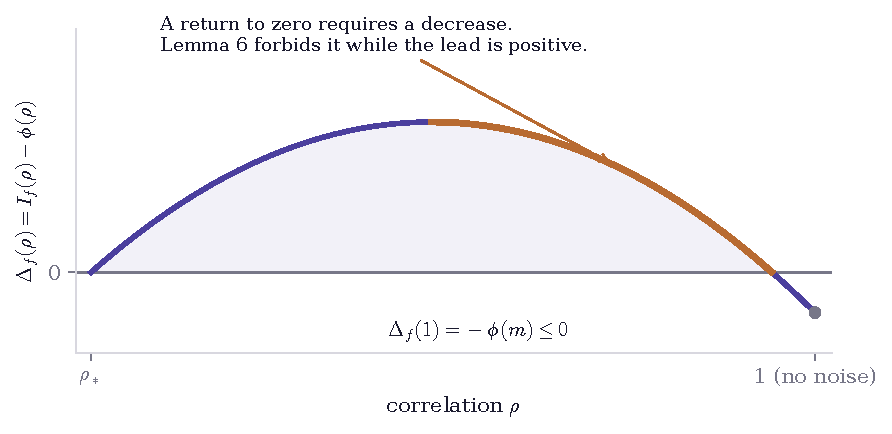
\includegraphics[width=.94\linewidth]{maximum.pdf}
\caption{Schematic of the growth contradiction. A positive lead would
have to decrease before reaching its nonpositive value at \(\rho=1\),
whereas Lemma~\ref{lem:coverage} shows that it is strictly increasing
whenever it is positive.}
\label{fig:growth-contradiction}
\end{figure}

For a putative violation, the information premise is exactly
\begin{equation}
 \E h(T_\rho f)<h(\rho)-\phi(m).                         \label{eq:premises}
\end{equation}
It supplies a positive credit in the spectral baseline. Our target is
\(A(u)>\rho\logodds\), with \(\logodds=\atanh\rho\):
by \eqref{eq:action}, this says that the lead is increasing.

\section{Edge Geometry and the Pivotal Decomposition}
\label{sec:edges}

For a coordinate index \(i\), let \(f_{i,+}\) and \(f_{i,-}\) be the
sections obtained by fixing that input to \(+1\) and \(-1\), respectively.
For a monotone Boolean function, the derivative in coordinate \(i\),
viewed on the other \(n-1\) coordinates, is
\[
 q_i^f=\frac{f_{i,+}-f_{i,-}}2\in\{0,1\}.
\]
It indicates a pivotal edge: one on which the output changes.
The influence \(\Inf_i(f)\) is the probability of such an edge.
Its mean
\[
 a_i=\E q_i^f=\widehat f(\{i\})=\Inf_i(f)
\]
is both the singleton Fourier coefficient and the influence.
This identity is special to monotone Boolean functions. After noise,
\(\E(u_{i,+}-u_{i,-})/2=\rho a_i\).
For a dictator, \(f_{1,+}=1\) and \(f_{1,-}=-1\), so
\(q_1^f=1\) everywhere; every other \(q_i^f\) is zero.
Retaining the indicator \(q_i^f\), rather than just its mean, will be
essential. Moment relaxations of the posterior can admit objects that
are not Boolean noise images, a distinction also examined
in~\cite[Section 8.1.2]{Gemini}. Our logarithmic Sobolev step acts on
the actual pivotal indicator and its positive smoothings.

For an edge with endpoint values \(p,q\), the action and angle energy
contributions are
\begin{align*}
 a(p,q)&=\frac{(p-q)(g(p)-g(q))}{4},\\
 j(p,q)&=\frac{(\arcsin p-\arcsin q)^2}{4}.
\end{align*}
Average over the edges in each coordinate direction, then sum over
directions. The results are \(A(u)\) and
\(\E[\Theta \Lapl \Theta]\), with \(\Theta=\arcsin u\).
Cauchy--Schwarz gives \(a\ge j\). We need a stronger statement which
keeps track of the difference.

\begin{remark}[Angular parametrization]
The derivative of \(g\) is \(g'(r)=1/(1-r^2)\).
Its square root is the derivative of \(\arcsin r\). For \(p\ge q\),
\[
 \left(\int_q^p\frac{\diff r}{\sqrt{1-r^2}}\right)^2
 \le (p-q)\int_q^p\frac{\diff r}{1-r^2}.
\]
This is exactly \(j(p,q)\le a(p,q)\). The angle turns an edge's
information cost into a squared difference, which Fourier analysis can
handle. The lemma retains the cost left over in this conversion.
\end{remark}

Define
\[
 F(v)=\frac{h(\tanh v)}{\tanh v},\qquad
 c(v)=\frac{\arcsin(\tanh v)^2}{\tanh v}.
\]
The function \(F\) decreases from infinity to zero. An entropy budget
\(H_{\rm budget}>0\) sets the centered comparison pair for each active
coordinate: its values are \(\pm\tanh v_i\), where
\[
                    F(v_i)=\frac{H_{\rm budget}}{\rho a_i}.
\]
This matches entropy per unit width. The comparison height \(v_i\)
is not a posterior observed on an individual edge. A smaller entropy
budget gives a larger height and a stronger growth bound.

The first bound below is the entropy-constrained edge envelope of
Chen--Gohari--Nair~\cite[Theorem 4 and Appendix C]{CGN}, written for
signs and natural logarithms. We also need the angle correction,
whose derivation is supplied in Appendix~\ref{app:scalar}.
No conjectured inequality from that paper is assumed.
The difference from its potential-induction program is where the
remaining cost is paid: here the edge correction is combined with
Fourier information from the same Boolean rule.

The same centered comparison pair will control both the total growth and
the residual growth after subtracting the angle energy. Using a common
entropy budget in the two bounds is essential for combining them later.

\begin{lemma}[The edge budget]\label{lem:edges}
Let \(f\) be nonconstant and monotone, \(0<\rho<1\), and
\(u=T_\rho f\). Choose any entropy budget
\(H_{\rm budget}\ge\E h(u)>0\). For every coordinate with
\(a_i>0\), define \(v_i\) by
\(F(v_i)=H_{\rm budget}/(\rho a_i)\). Then
\begin{align}
 A(u)&\ge\rho\sum_i a_i v_i,                         \label{eq:edge-budget}\\
 A(u)&\ge\E[\Theta\Lapl\Theta]
           +\rho\sum_i a_i\bigl(v_i-c(v_i)\bigr).   \label{eq:correction}
\end{align}
Coordinates with \(a_i=0\) contribute zero and are omitted.
\end{lemma}

\begin{proof}
For one edge put \(\edgewidth=|p-q|/2\) and
\(H_e=[h(p)+h(q)]/2\). The notation \(F^{-1}\) means the inverse
of the decreasing profile \(F\), not its reciprocal. Define the
correction function \(\corr\) by \(\corr(F(v))=v-c(v)\).
The scalar calculation in Appendix~\ref{app:scalar} proves
\begin{align*}
 a(p,q)&\ge\edgewidth F^{-1}(H_e/\edgewidth),\\
 a(p,q)-j(p,q)&\ge\edgewidth\corr(H_e/\edgewidth).
\end{align*}
Both right sides are convex in \((\edgewidth,H_e)\) and decrease
with \(H_e\). For coordinate \(i\),
\(\E\edgewidth=\rho a_i\) and
\(\E H_e=\E h(u)\le H_{\rm budget}\).
Jensen therefore bounds the two averaged edge costs below by their
values at \((\rho a_i,H_{\rm budget})\). Their inverse parameter
is exactly \(v_i\). Summing over coordinates proves both claims.
\end{proof}

For a dictator, choose its actual entropy \(H_{\rm budget}=h(\rho)\).
Put \(\theta=\arcsin\rho\). The sole height is
\(v_1=\atanh\rho\), and the two conclusions become
\(A=\rho\atanh\rho\) and
\(A=\theta^2+(\rho\atanh\rho-\theta^2)\). Thus the lemma preserves the
complete edge account, including the positive correction.

We use this lemma with two budgets. Whenever \(\E h(u)\le h(\rho)\),
the choice \(H_{\rm budget}=h(\rho)\) defines heights \(\ell_i\) by
\begin{equation}
                    F(\ell_i)=F(\logodds)/a_i.       \label{eq:heights}
\end{equation}
Since \(a_i\le1\), these satisfy \(0<\ell_i\le\logodds\).
The middle argument will use a smaller budget that also retains the
output mean; the lemma applies without changing its proof.

For the following illustration only, \(v\) is an edge-center parameter
and \(k>0\) its half-width in inverse-hyperbolic-tangent coordinates:
\(p=\tanh(v+k)\), \(q=\tanh(v-k)\).
These are local plot parameters. The plotted \(\edgewidth ,H_e,j\) are the
edge half-separation, average entropy, and angle cost defined above.

\begin{figure*}[t]
\centering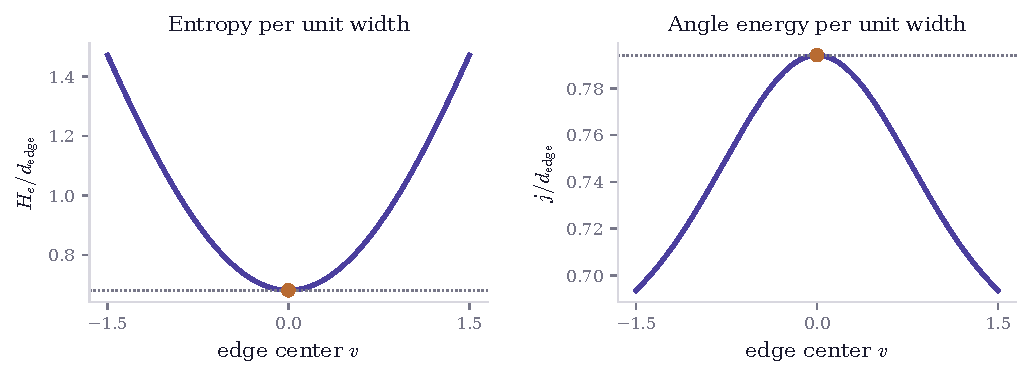
\includegraphics[width=.76\textwidth]{centered-edge.pdf}
\caption{The geometry behind the edge lemma. Write the endpoints as
\(p=\tanh(v+k)\), \(q=\tanh(v-k)\), with \(k=0.8\) in this illustration.
Centering at \(v=0\) minimizes entropy per unit width and maximizes
angle energy per unit width. These two extremal facts give a convex
lower bound on the action left after angle energy is removed.}
\label{fig:centered-edge}
\end{figure*}

With this budget, the first inequality bounds the total comparison weight:
\begin{equation}
                     W:=\sum_i a_i \ell_i\le A(u)/\rho.           \label{eq:W}
\end{equation}
For a dictator there is one active coordinate, \(a_1=1\), \(\ell_1=\logodds \),
and equality holds. The second inequality will be combined with a
spectral lower bound. Keeping its correction is essential.

\section{Information Growth Across Channel Regimes}
\label{sec:pivotal-middle}

\subsection{Intermediate-Correlation Growth}

We first prove the required growth inequality on the intermediate range
\(31/20\le\ell=\atanh\rho\le7/2\). In this section write \(r=\rho\).
The idea is to keep the coordinates together. Logarithmic Sobolev gives
an entropy cost for their pivotal probabilities; the log-sum inequality
then combines that cost with the edge budget. We will not choose a
comparison Fourier degree or divide coordinates by influence.
The underlying entropy tool is Gross's cube logarithmic Sobolev
inequality~\cite{Gross,ODonnell}. Its use here is specific: the positive
kernel in the next calculation converts pivotal-set entropy into the
same spectral expression produced by the centered angle comparison.
This supplies the correction left after the entropy-flow edge
bound~\cite{CGN}, without a conjectured coupling potential.


\begin{proposition}[Pivotal entropy forces faster growth]
\label{prop:middle-growth}
Let \(f\) be monotone Boolean and
\(31/20\le\atanh\rho\le7/2\). Then
\[
 I_f(\rho)>\phi(\rho)\quad\Longrightarrow\quad
 I_f'(\rho)>\phi'(\rho).
\]
The mean of \(f\) is unrestricted.
\end{proposition}

The proof compares the energy demanded by the information premise with
the growth available along the cube edges. It first obtains an
angle-energy requirement, expresses part of that requirement as pivotal
entropy, and then combines the entropy with the edge correction through
the log-sum inequality.

Put \(\Theta=\arcsin u\) and \(J_{\rm ang}=\E[\Theta\Lapl\Theta]\).
The dictator has posterior values \(\pm r\). Define its angle and the
slope of the line through those two angle values by
\[
 \theta=\arcsin r,\qquad \lambda=\theta/r.
\]
Two further coefficients come from the tangent inequality below:
\[
 \alpha=\frac{\theta+\sinh\ell}{\ell},\qquad
 \gamma=\lambda\alpha,\qquad
 \eta=\frac{\theta^2\gamma}{\gamma+1}.
\]
These are channel functions, not parameters to optimize.
The same \(\gamma\) will serve throughout the growth proof, including
the high-correlation extension. Only the way we estimate the pivotal
cost changes with the channel.

\subsubsection{Angle energy required by an information lead}

The following scalar inequality is proved in
Appendix~\ref{app:centered-support}:
\begin{equation}
 \begin{split}
 \frac{\alpha}{2}(\arcsin x-\lambda x)^2
 &\le x\arcsin x-r\theta\\
 &\quad-\alpha[\phi(x)-\phi(r)],qquad -1\le x\le1.
 \end{split}
 \label{eq:centered-support}
\end{equation}
Both sides vanish at \(x=\pm r\). It bounds the error of the
dictator's angle line by an entropy difference, without losing
equality at the reference posterior.
The comparison stays within Shannon entropy. Although the angle and
the Hellinger program~\cite{Hellinger,CN} both involve the geometry of
binary probabilities, we do not infer this inequality from a
Hellinger-optimality conjecture; its scalar proof is given in full.

Average \eqref{eq:centered-support} with \(x=u\), multiply by
\(2\lambda\), and complete the square in the positive operator
\(\Lapl+\gamma\). This gives
\begin{equation}
 \begin{split}
 J_{\rm ang}\ge{}&2\theta^2+2\gamma[\phi(m)+\Delta_f(r)]\\
 &+\lambda^2\E\left[u\left\{\gamma-
       \frac{(\gamma+1)^2}{\Lapl+\gamma}\right\}u\right].
 \end{split}
 \label{eq:centered-resolvent}
\end{equation}
Here division by \(\Lapl+\gamma\) means multiplication of each
degree-\(k\) Fourier coefficient by \(1/(k+\gamma)\).
For completeness, the discarded nonnegative square is
\begin{multline*}
 \E\bigl[
 \bigl(\Theta-\lambda(\gamma+1)(\Lapl+\gamma)^{-1}u\bigr)
 (\Lapl+\gamma)\\
 {}cdot\bigl(\Theta-\lambda(\gamma+1)
 (\Lapl+\gamma)^{-1}u\bigr)\bigr].
\end{multline*}
The constant Fourier mode is included; this matters when \(m\ne0\).
For the dictator, \(u=ry_1\) and \(\Theta=\lambda u\) are both
degree one. The operator \((\gamma+1)(\Lapl+\gamma)^{-1}\)
therefore fixes \(u\), so the discarded square is zero. In
\eqref{eq:centered-resolvent} the spectral term is \(-\theta^2\);
the result is exactly \(J_{\rm ang}=\theta^2\).

\subsubsection{Contribution of noisy pivotal sets}

Recall the pivotal indicator \(q_i^f\), with mean \(a_i\).
Omit coordinates with \(a_i=0\); every logarithm below then has a
positive argument.
Let \(t\in[0,r^2]\) denote a squared noise correlation and put
\[
 w_i(t)=T_{\sqrt t}q_i^f,\qquad s_i(t)=\E w_i(t)^2.
\]
Noise here acts on the other \(n-1\) coordinates.
The value \(w_i(t)\) is the conditional probability that coordinate
\(i\) is pivotal. Its mean remains \(a_i\); its second moment
\(s_i(t)\) records how unevenly that probability is distributed.
Complete averaging gives \(s_i(0)=a_i^2\), whereas the unsmoothed
indicator has second moment \(a_i\).
Define an average of these second moments:
\[
 z_i=\frac{\gamma+1}{\gamma r^2}
       \int_0^{r^2}[1-(t/r^2)^\gamma]s_i(t)\,dt,
 \qquad Z=\sum_i z_i.
\]
The weight in this integral is nonnegative and has total mass one.
Thus \(a_i^2\le z_i\le a_i\): noise preserves the mean and cannot
increase the second moment of an indicator.

Write \(V_0=1-m^2\) for the Boolean variance and
\(U=\operatorname{Var}(u)/r^2\) for the normalized noisy variance.
Fourier expansion of the integral gives
\[
 Z=(\gamma+1)\sum_{k\ge1}
       \frac{r^{2(k-1)}}{\gamma+k}
       \sum_{|S|=k}\widehat f(S)^2,
 \qquad 0<Z\le U\le V_0.
\]
The last inequality is Boolean Parseval followed by noise contraction.
For a dictator, \(w_1(t)=s_1(t)=z_1=1\), all other
coordinate terms vanish, and \(Z=U=V_0=1\). Thus \(V_0-Z\)
measures a variance reserve that is absent in the equality example.
The exact integral identity
\begin{align*}
 &\frac{\gamma+1}{\gamma}
 \int_0^{r^2}[1-(t/r^2)^\gamma]
       \sum_i\E[w_i(t)\Lapl w_i(t)]\,dt\\
 &\hspace{7em}=(\gamma+1)r^2(U-Z)
\end{align*}
is checked one Fourier degree at a time: a degree-\(k\) coefficient
appears in \(k\) pivotal derivatives, each of degree \(k-1\).

Cube logarithmic Sobolev, proved in Appendix~\ref{app:scalar}, gives
\[
 \E[w_i\Lapl w_i]\ge
       \frac12 s_i\log\frac{s_i}{a_i^2}.
\]
For the auxiliary entropy bound, average under the probability
density \(w_i^2/s_i\). Jensen applied to \(\log(1/w_i)\) gives
\(\E_*\log w_i\ge\log(s_i/a_i)\), hence
\(\operatorname{Ent}(w_i^2)\ge s_i\log(s_i/a_i^2)\).
Here \(\operatorname{Ent}(v)=\E(v\log v)-(\E v)\log(\E v)\);
zero-weight points are omitted. Convexity of \(s\log(s/a_i^2)\)
and the averaging integral therefore give a bound on the
\emph{pivotal entropy cost}, defined by
\[
 E_{\rm piv}:=\sum_i z_i\log\frac{z_i}{a_i^2}.
\]
Each summand is nonnegative since \(z_i\ge a_i^2\); a noisy pivotal
probability that is constant has zero cost. In this notation,
\begin{equation}
 (\gamma+1)(U-Z)\ge\frac12 E_{\rm piv}.
 \label{eq:pivotal-entropy}
\end{equation}

Rewrite \eqref{eq:centered-resolvent} in terms of \(U,Z,V_0\), including
its constant mode, and then apply \eqref{eq:pivotal-entropy}.
To keep the bias contribution visible, define
\[
 M(m):=2\gamma\phi(m)-[\lambda^2(2-r^2)+\lambda/\alpha]m^2.
\]
The required angle energy is now
\begin{align}
 J_{\rm ang}
 &\ge\theta^2[1+V_0+\gamma U-(\gamma+1)Z]
          +M(m)+2\gamma\Delta_f(r)\notag\\
 &\ge\theta^2(1+V_0-Z)+\frac{\eta}{2}E_{\rm piv}
          +M(m)+2\gamma\Delta_f(r).                 \label{eq:pivotal-baseline}
\end{align}
Read the last line term by term: the dictator's energy \(\theta^2\),
the variance reserve \(\theta^2(V_0-Z)\), the pivotal entropy cost,
the bias correction, and the credit \(2\gamma\Delta_f(r)\) for extra
information. The last credit is strictly positive under a lead.
For the dictator, \(E_{\rm piv}=1\log1=0\), and every term except
\(\theta^2\) vanishes.

\subsubsection{Log-sum closure of the edge budget}

Suppose the information lead \(\Delta=\Delta_f(r)\) is positive,
but its growth is no faster than the dictator's: \(A(u)\le r\ell\).
We derive a contradiction.
Monotonicity gives \(a_i\le1-|m|\le V_0\). Also
\[
 \E h(u)=h(r)-\phi(m)-\Delta\le V_0h(r),
\]
since \(\phi(m)\ge m^2/2\) and \(h(r)<1/2\).
For the latter, \(r>9/10\) and \(L<7/10\) give
\(h(r)\le L-r^2/2<1/2\).
Apply Lemma~\ref{lem:edges} with
\(H_{\rm budget}=V_0h(r)\). Its heights satisfy
\[
 F(v_i)=\frac{V_0h(r)}{r a_i}=\frac{V_0F(\ell)}{a_i},
 \qquad 0<v_i\le\ell,
\]
where the upper bound follows from \(a_i\le V_0\) and the decrease
of \(F\). With \(H(v)=v-c(v)\), the lemma gives
\begin{equation}
 \sum_i a_i v_i\le A(u)/r\le\ell,\qquad
 A(u)\ge J_{\rm ang}+r\sum_i a_iH(v_i).
 \label{eq:adjusted-edge}
\end{equation}
These heights are comparison parameters; they are not additional
properties assumed of the field.

Set \(\beta=2r/\eta\). The channel estimates proved in
Lemma~\ref{lem:middle-channel-checks} are
\begin{align}
 \log\frac{vF(v)}{\ell F(\ell)}
       &\ge\beta[H(\ell)-H(v)] &&(0<v\le\ell), \label{eq:middle-profile}\\
 \theta^2-rH(\ell)-\eta/2&\ge0,                \label{eq:middle-energy}\\
 M(m)-rH(\ell)m^2&\ge0.                       \label{eq:middle-mean}
\end{align}
Their role is simple: the first converts the edge budget to a
normalization for log-sum; the other two leave nonnegative reserves.

For that normalization, put
\(b_i=a_i^2e^{-\beta H(v_i)}\) and \(B_{\rm piv}=\sum_i b_i\).
This choice puts the edge correction inside the entropy logarithm:
\(\log(z_i/b_i)=\log(z_i/a_i^2)+\beta H(v_i)\).
The weights need not sum to one; log-sum keeps track of their total.
Equation~\eqref{eq:middle-profile} gives
\[
 \frac{b_i}{a_iv_i}
 \le\frac{V_0}{\ell}e^{-\beta H(\ell)},\qquad
 B_{\rm piv}\le V_0e^{-\beta H(\ell)}.
\]
The second inequality uses the first bound in
\eqref{eq:adjusted-edge}: a rule growing no faster than the dictator
has only \(\ell\) units of edge weight to allocate.
Since \(z_i\le a_i\), \(H\ge0\), and
\(\eta\beta/2=r\), log-sum now yields
\begin{align*}
 \frac{\eta}{2}E_{\rm piv}+r\sum_i a_iH(v_i)
 &\ge\frac{\eta}{2}\sum_i z_i\log\frac{z_i}{b_i}\\
 &\ge\frac{\eta}{2}Z\log\frac Z{B_{\rm piv}}\\
 &\ge\frac{\eta}{2}Z\log\frac Z{V_0}+rZH(\ell).
\end{align*}
The first line joins the two costs by the logarithmic identity just
given. The second is log-sum. The third uses the bound on total weight.
This is the connection between the information requirement and the
available growth: both involve the same noisy pivotal sets.

Finally insert this bound into \eqref{eq:pivotal-baseline} and
\eqref{eq:adjusted-edge}. Subtract
\(r\ell=\theta^2+rH(\ell)\), and use
\(Z\log(Z/V_0)\ge Z-V_0\), the tangent inequality for \(t\log t\):
\begin{equation}
 \begin{aligned}
 A(u)-r\ell\ge{}&
 \underbrace{[\theta^2-rH(\ell)-\eta/2](V_0-Z)}_{
                    \text{nonnegative variance reserve}}\\
 &+\underbrace{[M(m)-rH(\ell)m^2]}_{\text{nonnegative bias reserve}}
  +\underbrace{2\gamma\Delta}_{\text{positive lead credit}}>0.
 \end{aligned}
 \label{eq:pivotal-growth-account}
\end{equation}
This contradicts \(A(u)\le r\ell\). We have proved
\[
 \Delta_f(r)>0\ \Longrightarrow\ A(u)>r\ell
 \qquad(31/20\le\ell\le7/2).
\]
At a dictator, \(a_1=z_1=V_0=1\) and \(v_1=\ell\).
Log-sum has one term and is exact. The variance reserve, bias reserve,
and lead credit are all zero. What remains is the exact account
\[
 \underbrace{r\ell}_{\text{growth}}
   =\underbrace{\theta^2}_{\text{angle energy}}
    +\underbrace{rH(\ell)}_{\text{edge correction}}.
\]
An information lead would add the strictly positive last term in
\eqref{eq:pivotal-growth-account}; the other two terms cannot cancel it.


\subsection{High-Correlation Spectral Regime}
The intermediate-correlation argument pays for the edge correction from
an angle reserve. The dictator's
squared angle \(\theta^2\) stays below \(\pi^2/4\), while its edge
correction \(\ell-c(\ell)\) grows without bound. That reserve cannot
cover the whole tail. For \(\ell\ge7/2\), we keep the same angle
inequality, completed square, and penalty, but estimate the spectral
term by comparison with a reference Fourier degree.

\subsection{Coordinate Deficit Bounds}
\label{sec:coordinate}

Keep the canonical penalty \(\gamma=\lambda\alpha\) from the centered
angle comparison. We introduce only a comparison degree \(\degree\ge2\),
which may be real rather than integer. In the tail we choose
\(\degree=\ell/2+5/4\); every coordinate uses the same degree. Define
\begin{align*}
 \weight(s)&=\frac{\gamma s}{\gamma+s},\\
 \Klsi&=\frac{\gamma^2e^{2\degree-3}}
              {2(\gamma+\degree)(\gamma+1)},\\
 d_1&=[\weight(\degree)-\weight(1)]\rho^2,\\
 d_2&=[\weight(\degree)-\weight(2)]\rho^4.
\end{align*}
The bounded spectral weight \(\weight(s)\) will arise from completing a square.
We replace \(\weight(|S|)\) by the common value \(\weight(\degree )\).
One estimate for the resulting loss uses the entropy of the noisy
pivotal set, while the other uses the total energy of its indicator.
Neither bound dominates uniformly, so both are retained.

\begin{lemma}[Two bounds for the coordinate deficit]\label{lem:deficit}
Set
\begin{align*}
 D_i&=\sum_{S\ni i}
       \frac{\weight(\degree)-\weight(|S|)}{|S|}\widehat u(S)^2,\\
 D(a)&=\min\left\{\Klsi\rho^2a^2,
       \frac{d_2}{2}a+\left(d_1-\frac{d_2}{2}\right)a^2\right\}.
\end{align*}
For a monotone Boolean noise image, \(D_i\le D(a_i)\). Consequently,
\begin{equation}
 \sum_{S\ne\varnothing}\weight(|S|)\widehat u(S)^2
       \ge \weight(\degree )(\E u^2-m^2)-\sum_iD(a_i).             \label{eq:spectral}
\end{equation}
\end{lemma}

\subsubsection{Logarithmic-Sobolev bound via positive smoothing}

For a nonnegative cube function \(v\), define
\(\Ent(v)=\E[v\log v]-(\E v)\log(\E v)\), with \(0\log0=0\).
For any real-valued cube function \(w\), the standard cube
logarithmic Sobolev inequality (LSI) \cite{Gross,ODonnell} is
\[
 \Ent(w^2)\le2\E[w\Lapl w].
\]
It holds in every dimension with the same constant; a complete
two-point and tensorization proof is in Section~\ref{app:lsi-proof}.
For nonzero, nonnegative \(w\), let \(s=\E w^2\) and \(b=\E w\).
Weight each cube point by \(w^2/s\), and denote expectation under this
probability measure by \(\E_*\). Jensen gives
\[
 \E_*\log w=-\E_*\log(1/w)
       \ge-\log\E_*(1/w)=\log(s/b).
\]
Points where \(w=0\) have zero weight. It follows that
\(\Ent(w^2)=s(2\E_*\log w-\log s)\ge s\log(s/b^2)\).
The logarithmic Sobolev bound therefore gives
\[
 \E[w(\Lapl+1-\degree)w]
 \ge\frac{s}{2}\log\frac{s}{b^2}+(1-\degree)s.
\]
The right side is minimized at \(s=b^2e^{2\degree-3}\), giving
\begin{equation}
 \E[w(\Lapl +1-\degree )w]\ge-\frac12e^{2\degree -3}(\E w)^2.
 \label{eq:defective-lsi}
\end{equation}
The zero function is handled by continuity.

Now average this inequality over ordinary noise smoothings of the
coordinate derivative. Let \(\Lapl_{-i}\) be the Laplacian on the
coordinates other than \(i\), and, for \(0\le t\le1\), set
\[
 p_i=\frac{u_{i,+}-u_{i,-}}2,\qquad w_t=T_{\sqrt t}p_i.
\]
Monotonicity gives \(p_i\ge0\), so \(w_t\ge0\), and every smoothing
has the same mean \(\E w_t=\rho a_i\). There is an exact identity:
\[
 D_i=\frac{\gamma}{\gamma+\degree}
 \int_0^1(1-t^\gamma)
     \E\bigl[w_t(\degree-1-\Lapl_{-i})w_t\bigr]\,\diff t.
\]
To check it, a Fourier set \(S\ni i\) of size \(s\) becomes a set
of size \(s-1\) after taking the derivative. Its squared coefficient
in \(w_t\) is \(t^{s-1}\widehat u(S)^2\), and
\begin{align*}
 &\frac{\gamma(\degree-s)}{\gamma+\degree}
       \int_0^1(1-t^\gamma)t^{s-1}\,\diff t\\
 &\hspace{2em}=\frac{\gamma^2(\degree-s)}
 { (\gamma+\degree)s(\gamma+s)}
 =\frac{\weight(\degree)-\weight(s)}s.
\end{align*}
This is precisely its coefficient in \(D_i\).

Apply \eqref{eq:defective-lsi} to each \(w_t\). The expectation in
the integral is at most \(e^{2\degree-3}(\rho a_i)^2/2\).
Since \(\int_0^1(1-t^\gamma)\,\diff t=\gamma/(\gamma+1)\),
we obtain \(D_i\le\Klsi\rho^2a_i^2\).

\begin{remark}[Noise averaging]
The integral creates exactly the spectral weight defining the deficit.
Every field in the average stays nonnegative and has the same mean,
so the same logarithmic Sobolev estimate applies throughout.
\end{remark}
Samorodnitsky's noisy-function entropy estimates~\cite{SamEntropy}
likewise exploit structure preserved under noise. The calculation here
uses the standard LSI directly: its positive integral is chosen to
reproduce the displayed resolvent weight, so no separate
hypercontractive approximation of that weight is required.

\subsubsection{Indicator-energy bound}

The unsmoothed derivative \(q_i^f\) is an indicator with mean \(a_i\).
Its total Fourier energy is \(a_i\); its constant coefficient contributes
\(a_i^2\). Therefore
\[
 \sum_{S\ni i}\frac{\widehat f(S)^2}{|S|}
                   \le a_i^2+\frac12(a_i-a_i^2)
                   =\frac{a_i+a_i^2}{2}.
\]
For degrees \(s\ge2\), the coefficient
\([\weight(\degree )-\weight(s)]\rho^{2s}\) is at most \(d_2\ge0\).
If it is negative this is immediate. Otherwise \(2\le s<\degree\), and
\[
 \weight(\degree)-\weight(s)
 =\frac{\gamma^2(\degree-s)}{(\gamma+\degree)(\gamma+s)}.
\]
On the positive interval, the only \(s\)-dependent factor decreases,
because
\[
 \frac{\diff}{\diff s}\log\frac{(\degree-s)\rho^{2s}}{\gamma+s}
 =-\frac1{\degree-s}+2\log\rho-\frac1{\gamma+s}<0.
\]
Hence its largest integer value occurs at degree two. Separate the
singleton contribution to obtain
\[
 D_i\le\frac{d_2}{2}(a_i+a_i^2)+(d_1-d_2)a_i^2.
\]
This proves both bounds in Lemma~\ref{lem:deficit}. Finally, summing \(D_i\)
counts every nonempty set \(S\) exactly \(|S|\) times against its factor
\(1/|S|\). The cancellation gives \eqref{eq:spectral}.

\subsection{Entropy-Funded Spectral Baseline}
\label{sec:baseline}

The centered angle comparison \eqref{eq:centered-resolvent} is valid
for every \(\ell\ge31/20\), not just the middle range. We now combine
it with the coordinate deficits. Write \(\Theta=\arcsin u\) for the
angle field and \(\theta=\arcsin\rho\) for the dictator's angle, and set
\[
 p=(\lambda+1/\alpha)^2,\qquad
 b=\lambda^2(2+1/\gamma),\qquad
 C_d=p\weight(\degree)-b.
\]
From this point onward, \(p\) denotes this spectral multiplier, not an
endpoint value from the earlier edge calculation.
The coefficient \(p\) comes from the same completed square as before;
no new angle approximation or penalty is introduced. Define
\[
 B=2\theta^2+C_d\frac{\phi(\rho)}L,\qquad
 k_\Delta=2\gamma+\frac{C_d}L.
\]
The information premise bounds the noisy second moment below, with
a bound that increases with the lead. When \(C_d\ge0\), that gives
an additional positive contribution to the angle energy.

The next lemma lower-bounds the required angle energy after accounting
for the coordinate losses. Its two conditions have separate roles: the
first permits the second-moment
substitution, and the second makes the remaining bias contribution
nonnegative. They are proved for the chosen channel parameters in the tail
appendix, rather than assumed as properties of the Boolean rule.

\begin{lemma}[An entropy-funded spectral baseline]\label{lem:baseline}
Let \(u=T_\rho f\) for a monotone Boolean function \(f\), with
\(\ell=\atanh\rho\ge31/20\) and the canonical penalty
\(\gamma=\lambda\alpha\). Suppose
\begin{equation}
 C_d\ge0,\qquad
 \gamma-b+C_d\left(\frac1{2L}-1\right)\ge0.
 \label{eq:canonical-baseline-conditions}
\end{equation}
Then
\begin{equation}
 \E[\Theta\Lapl\Theta]\ge B-p\sum_iD(a_i)
                           +k_\Delta\Delta_f(\rho).
 \label{eq:baseline}
\end{equation}
\end{lemma}

\begin{proof}
The identity \(\gamma=\lambda\alpha\) gives, for every degree \(s\ge0\),
\[
 \lambda^2\left[\gamma-\frac{(\gamma+1)^2}{\gamma+s}\right]
                         =p\weight(s)-b.
\]
Insert it into \eqref{eq:centered-resolvent}, including the constant
mode, and then use Lemma~\ref{lem:deficit}:
\begin{align*}
 \E[\Theta\Lapl\Theta]\ge{}&
 2\theta^2+C_d\operatorname{Var}(u)-p\sum_iD(a_i)\\
 &+2\gamma\phi(m)-b m^2+2\gamma\Delta_f(\rho).
\end{align*}
The entropy series bounds \(\phi(t)\le Lt^2\) on \([-1,1]\):
\[
 \phi(t)=\sum_{j\ge1}\frac{t^{2j}}{2j(2j-1)}
 \le t^2\sum_{j\ge1}\frac1{2j(2j-1)}=Lt^2.
\]
As \(\E\phi(u)=\phi(\rho)+\phi(m)+\Delta_f(\rho)\), this yields
\[
 \operatorname{Var}(u)\ge
 \frac{\phi(\rho)+\phi(m)+\Delta_f(\rho)}L-m^2.
\]
Its coefficient \(C_d\) is nonnegative, so substitution preserves the
lower bound. The channel and lead terms are \(B\) and
\(k_\Delta\Delta_f(\rho)\). The remaining mean term is exactly
\begin{align*}
 &\left(2\gamma+\frac{C_d}L\right)\phi(m)-(C_d+b)m^2\\
 &\quad\ge
 \left[\gamma-b+C_d\left(\frac1{2L}-1\right)\right]m^2\ge0,
\end{align*}
using \(\phi(m)\ge m^2/2\). Dropping only this nonnegative term proves
the claim. No sign assumption on \(\Delta_f\) was needed.
\end{proof}

The mean was never set to zero. Conditions
\eqref{eq:canonical-baseline-conditions} give the signs needed to use
the second-moment bound and discard the mean remainder. The tail
appendix proves them for the canonical penalty and the displayed degree.

\subsection{Yield Comparison and Growth}
\label{sec:contradiction}

For \(0<v\le \logodds \), set \(a=F(\logodds )/F(v)\) and define
\[
 \unitcost(v)=\frac{\rho c(v)}v+\frac{pD(a)}{a v}.
\]
This \emph{allowed yield} is angle contribution plus Fourier loss,
per unit of edge weight \(av\). The \emph{required yield}
\(B/\logodds\) is the channel baseline per unit dictator weight.
These are comparison bounds, not coordinate mutual informations.

The next lemma shows that the coordinate losses cannot consume the extra
energy required by an information lead when every coordinate's allowed
yield is below the required yield. Its proof combines two accounts of the
same growth: angle energy plus correction and the total edge-weight budget.

\begin{lemma}[The yield comparison forces faster growth]\label{lem:budget}
Let \(u=T_\rho f\) for a monotone Boolean \(f\), with
\(\ell=\atanh\rho\ge31/20\) and the canonical penalty.
Assume \(\Delta_f(\rho)=I_f(\rho)-\phi(\rho)\ge0\) and the two
conditions \eqref{eq:canonical-baseline-conditions}.
If
\begin{equation}
 \frac B\logodds\ge\rho,\qquad
 \frac B\logodds\ge\unitcost(\ell_i)
 \quad\text{for every active coordinate }i,                 \label{eq:scalar-test}
\end{equation}
then
\begin{equation}
 \Delta_f'(\rho)\ge
       \frac{k_\Delta\logodds}{B}\,\Delta_f(\rho).
 \label{eq:final-budget}
\end{equation}
In particular, a positive information lead has positive growth.
\end{lemma}

\begin{proof}
The lead assumption gives
\(\E h(u)=h(\rho)-\phi(m)-\Delta_f(\rho)\le h(\rho)\),
so the edge lemma applies. Its correction and the spectral baseline
concern the same coordinate weights. Combining them gives
\begin{align*}
 A(u)&\ge\underbrace{\E[\Theta\Lapl\Theta]}_{\text{angle energy}}
         +\underbrace{\rho W-\rho\sum_i a_i c(\ell_i)}_{\text{edge correction}}\\
     &\ge \underbrace{B+k_\Delta\Delta_f(\rho)}_{\text{required baseline and lead credit}}
                  +\sum_i a_i\ell_i[\rho-\unitcost(\ell_i)]\\
     &\ge B+k_\Delta\Delta_f(\rho)
                  +\left(\rho-\frac B\logodds\right)W.
\end{align*}
The first line is Lemma~\ref{lem:edges}; the second inserts
Lemma~\ref{lem:baseline} and groups each coordinate's two costs into
its yield. The last line uses the scalar yield comparison. Thus the
many coordinate losses now depend only on the single total weight \(W\).
Now use the other edge bound, \(W\le A(u)/\rho\).
Its coefficient in the last line is nonpositive, so substitution gives
The resulting growth budget is
\begin{equation}
 \frac{B}{\rho\logodds}A(u)
 \ge B+k_\Delta\Delta_f(\rho).
 \label{eq:growth-budget-compact}
\end{equation}
Since \(B/\logodds\ge\rho>0\), dividing and using
\(\Delta_f'=A(u)/\rho-\logodds\) proves \eqref{eq:final-budget}.
The lead supplies the positive credit that forces its own growth.
Lemma~\ref{lem:coverage} establishes the scalar comparisons needed here.
\end{proof}

\section{Proof of the Main Theorem}
\label{sec:coverage}

We now state the conclusion in the variables of the original problem.
Recall that \(I_f(\rho)\) is the retained bit's mutual information,
\(\phi(\rho)\) is the dictator's information, and a prime means
\(d/d\rho\) with the function \(f\) fixed.



\subsection{Direct Bounds}

These bounds already settle two classes of possible counterexamples.
They are logically separate from the spectral comparison.

\begin{proposition}[Small correlation]\label{prop:low}
For every Boolean function \(f\), of any mean, and every
\(0\le\rho\le\rho_*\),
\[
                         I_f(\rho)\le\phi(\rho).
\]
\end{proposition}
\begin{proof}
Appendix~\ref{app:low} proves this from an elementary quantitative
Fourier estimate, an entropy minorant, and entropy contraction.
The supporting estimates are proved there and in
Appendix~\ref{app:scalar}.
\end{proof}

\begin{proposition}[A sufficiently influential coordinate]\label{prop:local}
Let \(f\) be Boolean, \(0<\rho<1\), and let
\(a=|\widehat f(\{i\})|\) for some coordinate \(i\).
If
\begin{equation}
 (1-\rho^2)h(\rho a)\ge(1-\rho^2a)h(\rho),
 \label{eq:local}
\end{equation}
then \(I_f(\rho)\le\phi(\rho)\).
\end{proposition}
\begin{proof}
This is the influential-coordinate part of the local/Fourier division
used by Yu~\cite[Section 4.2]{Yu}. Appendix~\ref{app:scalar} proves
the displayed criterion with its mean remainder retained. For monotone
\(f\), \(a\) is the coordinate's influence; dictators have \(a=1\)
and give equality.
\end{proof}

\subsection{Global Growth Comparison}

A violating function must have \(\rho>\rho_*\), and every one of
its coordinates must fail \eqref{eq:local}. Its coordinate influences
therefore lie in the domain of the yield comparison below.

\begin{lemma}[An advantage must be growing]\label{lem:coverage}
For every monotone Boolean function \(f\) and every \(0<\rho<1\),
\[
 I_f(\rho)>\phi(\rho)
      \quad\Longrightarrow\quad I_f'(\rho)>\phi'(\rho).
\]
In words: wherever a rule beats the dictator, its lead is increasing.
\end{lemma}

\begin{proof}
Proposition~\ref{prop:low} excludes \(\ell\le31/20\).
On \(31/20\le\ell\le7/2\), Section~\ref{sec:pivotal-middle}
proves the claim by the entropy and log-sum argument.
For \(\ell\ge7/2\), Proposition~\ref{prop:local} excludes the
influential-coordinate case. On all remaining coordinates,
Appendix~\ref{app:verification} proves, with the same canonical
penalty and \(\degree=\ell/2+5/4\), both conditions in
\eqref{eq:canonical-baseline-conditions} and
\begin{equation}
 B/\ell\ge\max\{\rho,\unitcost(v)\}
 \label{eq:coverage-scalar}
\end{equation}
for every retained height \(v\). The continuum of heights reduces
to the half-height join and the cutoff by
Appendix~\ref{app:endpoints}. Three half-line comparisons prove
the bounds, with no bounded cutoff ranges.
Lemma~\ref{lem:budget} now gives \(A(u)>\rho\ell\).
Since \(A(u)=\rho I_f'(\rho)\) and \(\phi'(\rho)=\ell\),
this is precisely the conclusion.
\end{proof}

\begin{proof}[Proof of Theorem~\ref{thm:CK}]
By Lemma~\ref{lem:sorting}, it suffices to consider monotone functions.
Fix one and write \(\Delta_f=I_f-\phi\). At the noiseless endpoint,
\(\Delta_f(1)=-\phi(m)\le0\).

Suppose \(\Delta_f\) is positive somewhere. Choose any point
\(\rho_0\) in a maximal open interval on which it is positive,
and call that interval's right endpoint \(b\le1\).
Lemma~\ref{lem:coverage} makes \(\Delta_f\) strictly increasing on
this interval. Consequently
\(\lim_{\rho\uparrow b}\Delta_f(\rho)\ge\Delta_f(\rho_0)>0\).
Continuity gives \(\Delta_f(b)=0\) if \(b<1\), or
\(\Delta_f(b)\le0\) if \(b=1\). Either case is a contradiction.
\end{proof}

\section{Vector-Valued Quantization and a Threshold at Eight Bits}
\label{sec:multibit-extension}

Theorem~\ref{thm:CK} motivates the vector-valued question of whether a
\(k\)-bit summary is optimized by retaining \(k\) input coordinates. The
answer is negative in general. This section gives explicit counterexamples,
describes their coding-theoretic mechanism, and isolates the range that
remains open.

The outcome is unexpectedly sharp. Shortened Hamming quantizers violate
the coordinate benchmark for \(k=8,9,10\), and hence, by adding independent
coordinate outputs, for every \(k\geq 8\). The same construction misses the
benchmark at \(k=7\) by only \(1/64\) in the high-noise coefficient. A broad
collection of searches below eight bits also failed to produce a violation.
This leads us to conjecture that the coordinate projection is optimal for
\(2\leq k\leq7\).

Throughout this section, entropies and mutual informations are measured in
bits. Let
\begin{align*}
 X&\sim\operatorname{Unif}(\mathbb F_2^n),\qquad Y=X\oplus Z,\\
 Z_i&\stackrel{\mathrm{iid}}{\sim}\operatorname{Bernoulli}(p),
 \qquad 0\leq p\leq\frac12.
\end{align*}
and write
\[
 h_2(p)=-p\log_2p-(1-p)\log_2(1-p),
 \qquad C(p)=1-h_2(p).
\]

\subsection{Problem Formulation and Known Results}

For \(n\geq k\), define
\begin{equation}
 M_k(n,p)
 :=\max_{f:\mathbb F_2^n\to\mathbb F_2^k} I(f(X);Y).
 \label{eq:multibit-Mkn}
\end{equation}
The \(k\)-coordinate projection
\[
 D_k(x)=(x_1,\ldots,x_k)
\]
satisfies \(I(D_k(X);Y)=kC(p)\). We call \(D_k\), and any version obtained
by permuting input coordinates and relabeling its \(2^k\) outputs, a
\emph{dictator tuple}. The most direct vector extension of the
Courtade--Kumar assertion is therefore
\begin{equation}
 M_k(n,p)\stackrel{?}{\leq} kC(p)
 \qquad\text{for every }n\geq k.
 \label{eq:vector-CK}
\end{equation}

There are three useful landmarks in the literature.

\begin{enumerate}
\item For \(k=1\), inequality~\eqref{eq:vector-CK} is the original
Courtade--Kumar conjecture~\cite{CK}, proved in this paper.

\item Huleihel and Ordentlich proved the complementary endpoint: for every
\(f:\mathbb F_2^n\to\mathbb F_2^{n-1}\),
\[
 I(f(X);Y)\leq(n-1)C(p).
\]
Their theorem also extends from the BSC to every binary-input memoryless
output-symmetric channel~\cite{HO}. Notice that this is an assertion with
\(k=n-1\), not an assertion for a fixed \(k\) and arbitrary \(n\); hence it
does not conflict with the fixed-\(k\) counterexamples below.

\item Chandar and Tchamkerten formulated the general optimization
problem~\eqref{eq:multibit-Mkn} and characterized its positive-rate
asymptotics~\cite{CT}. If \(k/n\to R\in(0,1)\), then
\begin{equation}
 \begin{split}
 \frac{M_k(n,p)}{n}&\longrightarrow
 1-h_2\!\left(p\star h_2^{-1}(1-R)\right),\\
 p\star q&=p(1-q)+(1-p)q.
 \end{split}
 \label{eq:CT-asymptotic}
\end{equation}
This limit can exceed \(RC(p)\), so the vector assertion cannot hold at
every positive rate. At finite blocklength, they exhibited violations
from the perfect \([15,11,3]\) Hamming code and the \([23,12,7]\) Golay
code. They also observed that the \([7,4,3]\) Hamming code does not
violate the bound and explicitly asked for constructions with \(k<11\).
\end{enumerate}

One elementary point prevents a possible misunderstanding: a linear
\emph{code} can produce a nonlinear \emph{quantizer}.

\begin{proposition}[Affine maps obey the coordinate bound]
\label{prop:affine-multibit}
If \(f(x)=Ax+b\) is affine, with output rank \(r\leq k\), then
\[
 I(f(X);Y)\leq rC(p)\leq kC(p).
\]
\end{proposition}

\begin{proof}
It is enough to treat a rank-\(r\) linear map. Since \(X\) is uniform,
\(AX\) is uniform on \(\mathbb F_2^r\). Moreover, \(Z=X\oplus Y\) is
independent of \(Y\), and hence
\[
 I(AX;Y)=r-H(AZ).
\]
Choose \(r\) columns of \(A\) that form an invertible submatrix and call
their index set \(J\). Conditioning on \(Z_{J^c}\), the variable \(AZ\)
is a translate of an invertible image of \(Z_J\). Consequently,
\[
 H(AZ)\geq H(AZ\mid Z_{J^c})=H(Z_J)=r h_2(p),
\]
which proves the claim.
\end{proof}

Thus every counterexample must use genuine nonlinearity. The constructions
below use linear codebooks, but the nearest-codeword map into those
codebooks is nonlinear.

\subsection{Coset Quantizers and the High-Noise Expansion}
\label{subsec:coset-diagnostic}

Let \(C\leq\mathbb F_2^n\) be a binary linear code of dimension \(k\),
with full-rank parity-check matrix \(H\in\mathbb F_2^{(n-k)\times n}\).
For each syndrome \(a\in\mathbb F_2^{n-k}\), choose a minimum-weight
coset leader \(e_a\) satisfying \(He_a=a\), with \(e_0=0\), and define
\begin{equation}
 Q(x)=x\oplus e_{Hx}\in C.
 \label{eq:coset-quantizer}
\end{equation}
After composing \(Q\) with any bijection from \(C\) to
\(\mathbb F_2^k\), this is a \(k\)-bit quantizer. The choice among tied
minimum-weight leaders is part of the construction.

If \(X\) is uniform, the change of variables
\[
 X=Q(X)\oplus E,
 \qquad E=e_{HX},
\]
makes \(Q(X)\) uniform on \(C\), makes \(E\) uniform on the set of coset
leaders, and makes the two variables independent. Since \(Y\) is uniform
on \(\mathbb F_2^n\), translation invariance gives the exact identity
\begin{equation}
 I(Q(X);Y)=n-H(E\oplus Z).
 \label{eq:coset-information}
\end{equation}
This reduces the entire information calculation to the entropy of a noisy
coset leader.

Set \(\rho=1-2p\) and define
\begin{equation}
 B(E):=\sum_{j=1}^n
 \left(\mathbb E[(-1)^{E_j}]\right)^2.
 \label{eq:leader-B}
\end{equation}
For a set \(S\), the Walsh coefficient of \(E\oplus Z\) is
\[
 \rho^{|S|}\mathbb E\!\left[(-1)^{\sum_{j\in S}E_j}\right].
\]
Expanding relative entropy from the uniform distribution at \(\rho=0\)
therefore yields
\begin{align}
 I(Q(X);Y)
 &=\frac{\rho^2}{2\ln2}B(E)+O(\rho^4),
 \label{eq:code-high-noise}\\
 kC(p)
 &=\frac{\rho^2}{2\ln2}k+O(\rho^4).
 \label{eq:benchmark-high-noise}
\end{align}
In particular,
\begin{equation}
 \begin{split}
 B(E)>k\quad\Longrightarrow\quad I(Q(X);Y)>kC(p)\\
 \text{for all \(p<1/2\) sufficiently close to \(1/2\)}.
 \end{split}
 \label{eq:B-counterexample}
\end{equation}
This exact second-order test is the main design criterion used below.

\subsection{Shortened-Hamming Counterexamples for
\texorpdfstring{\(k=8,9,10\)}{k=8,9,10}}
\label{subsec:shortened-hamming}

Identify the nonzero vectors of \(\mathbb F_2^4\) with the integers
\(1,\ldots,15\) through their binary expansions. For
\(s\in\{1,2,3\}\), let \(H_s\) have as its columns
\[
 \{s+1,s+2,\ldots,15\}.
\]
Thus \(C_s=\ker H_s\) is the shortened Hamming code
\begin{equation}
 C_s=[15-s,11-s,3],
 \qquad n=15-s,
 \qquad k=11-s.
 \label{eq:shortened-Hamming-parameters}
\end{equation}

The retained syndrome \(8\) will be an anchor. Choose the following
minimum-weight leader for every syndrome \(a\in\mathbb F_2^4\):
\begin{equation}
 e_a=
 \begin{cases}
 0, & a=0,\\
 \mathbf e_a, & a\in\{s+1,\ldots,15\},\\
 \mathbf e_8\oplus\mathbf e_{8\oplus a}, & a\in\{1,\ldots,s\}.
 \end{cases}
 \label{eq:star-leaders}
\end{equation}
Here \(\mathbf e_a\) denotes the unit vector in the coordinate whose
parity-check column is \(a\). Both \(8\) and \(8\oplus a\) are retained.
The last line has syndrome \(a\), and it is minimum-weight because the
column \(a\) itself was removed. The missing syndromes therefore use
weight-two leaders that form a star around the common anchor \(8\).

The leader set consists of one word of weight zero, \(n\) words of weight
one, and \(s\) words of weight two. More importantly, the anchor occurs
in \(s+1\) leaders, each of the \(s\) leaves occurs in two leaders, and
each of the remaining \(14-2s\) coordinates occurs in one leader. Hence
\begin{align}
 B_s
 &=\left(1-\frac{s+1}{8}\right)^2
   +s\left(1-\frac{2}{8}\right)^2\notag\\
 &\quad +(14-2s)\left(1-\frac{1}{8}\right)^2\notag\\
 &=\frac{s^2-76s+735}{64},
 \label{eq:star-B}\\
 B_s-k
 &=\frac{s^2-12s+31}{64}.
 \label{eq:star-B-minus-k}
\end{align}

\begin{proposition}[Counterexamples below eleven bits]
\label{prop:k8-k10-counterexamples}
For each \(k\in\{8,9,10\}\), there are an \(n=k+4\), a quantizer
\(f:\mathbb F_2^n\to\mathbb F_2^k\), and an open interval of crossover
probabilities ending at \(1/2\) on which
\[
 I(f(X);Y)>kC(p).
\]
\end{proposition}

\begin{proof}
Use the quantizer~\eqref{eq:coset-quantizer} with the code and leaders in
\eqref{eq:shortened-Hamming-parameters}--\eqref{eq:star-leaders}. For
\(s=1,2,3\), corresponding respectively to \(k=10,9,8\),
\[
 B_s-k\in\left\{\frac5{16},\frac{11}{64},\frac1{16}\right\}>0.
\]
The conclusion follows from the high-noise expansion
\eqref{eq:B-counterexample}.
\end{proof}

\begin{proposition}[Failure for every \(k\geq8\)]
\label{cor:failure-all-k-ge-8}
For every integer \(k\geq8\), inequality~\eqref{eq:vector-CK} fails for
some input dimension and some \(p\in(0,1/2)\).
\end{proposition}

\begin{proof}
Start with the \(8\)-bit counterexample \(f_8\). For \(t=k-8\), append
\(t\) fresh independent input coordinates and define
\[
 F(x,u)=(f_8(x),u),
 \qquad u\in\mathbb F_2^t.
\]
The two channel blocks are independent, so
\[
 I(F(X,U);Y_X,Y_U)=I(f_8(X);Y_X)+tC(p)>kC(p).
\]
\end{proof}

The proof is analytic and uses only the sign of the exact rational number
\(B_s-k\). Direct entropy evaluation gives a more quantitative picture.
For \(y\in\mathbb F_2^n\), we computed
\begin{equation}
 \Pr(E\oplus Z=y)
 =\frac1{16}\sum_{a\in\mathbb F_2^4}
 p^{d_H(y,e_a)}(1-p)^{n-d_H(y,e_a)}
 \label{eq:direct-leader-convolution}
\end{equation}
and substituted the resulting distribution in
\eqref{eq:coset-information}. In Table~\ref{tab:shortened-hamming}, the
leader enumerator is
\(\sum_a z^{\operatorname{wt}(e_a)}\). The positive intervals and maxima
are numerical; the code parameters, leader enumerators, and \(B_s-k\)
are exact.

\begin{table*}[t]
\caption{Shortened-Hamming counterexamples. The code parameters,
leader enumerators, and high-noise excesses are exact; the intervals and
maxima are obtained by direct entropy evaluation.}
\label{tab:shortened-hamming}
\centering
{\footnotesize\setlength{\tabcolsep}{5pt}\renewcommand{\arraystretch}{1.12}
\begin{tabular}{@{}cccccc@{}}
\toprule
\(k\) & code & leader enumerator & \(B_s-k\) & numerical \(p\)-interval
& \(\max_p\Delta_k(p)/k\) \\ \midrule
10 & \([14,10,3]\) & \(1+14z+z^2\) & \(5/16\)
& \((0.088658,1/2)\) & \(4.48440\!\times\!10^{-3}\) \\
9 & \([13,9,3]\) & \(1+13z+2z^2\) & \(11/64\)
& \((0.152276,1/2)\) & \(1.83320\!\times\!10^{-3}\) \\
8 & \([12,8,3]\) & \(1+12z+3z^2\) & \(1/16\)
& \((0.265563,1/2)\) & \(3.21308\!\times\!10^{-4}\) \\
\bottomrule
\end{tabular}}
\end{table*}
Here
\[
 \Delta_k(p)=I(f(X);Y)-kC(p).
\]
The maximizing crossover probabilities are approximately \(0.199318\),
\(0.248809\), and \(0.332782\), respectively. Simple interior witness
points are
\begin{align*}
 \Delta_{10}(0.2)/10&=0.0044842878,\\
 \Delta_9(0.25)/9&=0.0018330159,\\
 \Delta_8(1/3)/8&=0.0003212940.
\end{align*}
Direct convolution and an independent Walsh-transform calculation agreed
to within \(10^{-14}\) at the tested crossover probabilities.

\begin{remark}[Order of shortening and decoding]
The successful operation is to remove columns from the Hamming
parity-check matrix and then choose a new minimum-weight syndrome table.
Deleting output bits after decoding with the full \([15,11,3]\) Hamming
quantizer is a different operation and did not reproduce these gains.
The shared anchor in~\eqref{eq:star-leaders} is also essential: it aligns
the coordinate biases that enter \(B(E)\).
\end{remark}

\subsection{Searches Below Eight Bits}
\label{subsec:below-eight-searches}

The star construction itself explains why eight is a natural boundary.
For \(s=4,5,6\), corresponding to \(k=7,6,5\), formula
\eqref{eq:star-B-minus-k} gives
\begin{table}[t]
\caption{High-noise coefficients of the shortened-Hamming family below
eight output bits.}
\label{tab:hamming-below-eight}
\centering
{\scriptsize\setlength{\tabcolsep}{3.5pt}\renewcommand{\arraystretch}{1.08}
\begin{tabular}{@{}ccccc@{}}
\toprule
\(k\) & \(n\) & leader enumerator & \(B_s\) & \(B_s-k\) \\ \midrule
7 & 11 & \(1+11z+4z^2\) & \(447/64\) & \(-1/64\) \\
6 & 10 & \(1+10z+5z^2\) & \(95/16\) & \(-1/16\) \\
5 & 9  & \(1+9z+6z^2\)  & \(315/64\) & \(-5/64\) \\
\bottomrule
\end{tabular}}
\end{table}
The seven-bit case is strikingly close: its leading high-noise term misses
the dictator tuple by only \(1/64\). A dense numerical evaluation found no
positive gap on \(0<p<1/2\); for example, the per-bit deficits at
\(p=0.1,0.2,0.4\) are respectively
\[
 0.0115176,\qquad 0.00410469,\qquad 0.000105113.
\]

We then tested several ways in which the Hamming near-miss might be
improved. Table~\ref{tab:k7-searches} records the scope of each computation and
the best high-noise statistic found. A negative-curve outcome means that
the full mutual-information curve was also evaluated on a dense grid and
at its numerical stationary candidates; it is not an analytic
impossibility proof.

\begin{table*}[t]
\caption{Computational searches for seven-bit code quantizers. A
``negative curve'' records dense numerical evaluation and stationary-point
checks, not an impossibility theorem for the corresponding family.}
\label{tab:k7-searches}
\centering
{\footnotesize\setlength{\tabcolsep}{4pt}\renewcommand{\arraystretch}{1.13}
\begin{tabular}{@{}
  >{\raggedright\arraybackslash}p{0.28\linewidth}
  >{\raggedright\arraybackslash}p{0.36\linewidth}
  >{\centering\arraybackslash}p{0.13\linewidth}
  >{\raggedright\arraybackslash}p{0.15\linewidth}@{}}
\toprule
Family & Search performed & best \(B\) & outcome \\ \midrule
Shortened Hamming, \(k=7\)
& All \(\binom{15}{4}=1365\) shortenings and all \(451{,}920\)
minimum-distance tie tables
& \(447/64\) & negative curve \\

Primitive BCH \([15,7,5]\)
& All \(1941\) puncturings deleting \(0,\ldots,4\) coordinates, with
multistart optimization of minimum-distance ties
& \(447/64\) & best case returns the Hamming near-miss \\

First- and second-order Reed--Muller family
& All \(651\) seven-dimensional codes
\(\mathrm{RM}(1,4)\subset C\subset\mathrm{RM}(2,4)\)
& \(6.850952\) & negative curves \\

Shortened binary Golay
& \(203\) sampled shortenings to dimension seven, with tie optimization
& \(6.895\) & negative curves \\

Random parity-check matrices
& \(345{,}000\) distinct-column searches with redundancies \(5,6,7,8\)
& \(447/64\) & no improvement over Hamming \\

Linear quotients of the \(k=8\) counterexample
& All \(255\) rank-seven quotients of the \([12,8,3]\) quantizer
& \(6.28125\) & negative curves \\
\bottomrule
\end{tabular}}
\end{table*}

We also tested repeated parity-check columns, nonminimum coset
representatives, the extended \([16,7,6]\) BCH construction, the
\([15,5,7]\) BCH code, and \(\mathrm{RM}(1,4)=[16,5,8]\). Repeated-column
searches occasionally reached \(B=7\), but only through a degeneracy whose
entire information curve equals that of seven independent dictators; no
strict gain appeared. Multistart searches over arbitrary coset
representatives likewise reached equality but not a violation.

These computations support a structural claim about the code-based
mechanism, not a theorem about all quantizers. In particular, the exact
exhaustion of Hamming tie tables certifies the best \(B\) only within that
family. A quantizer with a smaller high-noise coefficient could still,
in principle, cross the benchmark at an intermediate \(p\).

\subsection{Random Coding at \texorpdfstring{\(n=15,\ k=7\)}{n=15, k=7}}
\label{subsec:random-coding-k7}

The failed structured searches raise a natural question: is an unstructured
codebook more likely to find the missing gain? We tested the finite random
ensemble suggested by the rate-distortion picture. Choose a codebook
\(\mathcal C\) uniformly without replacement from all \(M=2^7\)-subsets of
\(\mathbb F_2^{15}\), map each input to a nearest codeword, and break each
tie independently and uniformly, once and for all.

Some geometric statistics of this ensemble are exact. Let
\[
 N=2^{15},\qquad
 S_d=\binom{15}{d},\qquad
 V_d=\sum_{i=0}^d S_i.
\]
For a fixed source word, let \(D\) be its distance to the random codebook
and \(T\) the number of codewords at that minimum distance. Then
\begin{align}
 \Pr(D>t)
 &=\frac{\binom{N-V_t}{M}}{\binom NM},
 \label{eq:random-distance-tail}\\
 \Pr(D=d,T=m)
 &=\frac{\binom{S_d}{m}\binom{N-V_d}{M-m}}{\binom NM}.
 \label{eq:random-distance-ties}
\end{align}
For \(n=15\) and \(M=128\), these formulas give
\begin{align*}
 \mathbb E D&=2.6608532,& \frac{\mathbb E D}{15}&=0.1773902,\\
 \Pr(T>1)&=0.4945889,& \mathbb E T&=2.1208972.
\end{align*}
Thus almost half of the source words have a nearest-neighbor tie.

For an arbitrary quantizer \(U=Q(X)\), not necessarily a coset quantizer,
the high-noise coefficient is
\begin{equation}
 B(Q)=\sum_{j=1}^n\sum_u\Pr(U=u)
 \left(\mathbb E[(-1)^{X_j}\mid U=u]\right)^2,
 \label{eq:general-B}
\end{equation}
and
\begin{equation}
 I(U;Y)=\frac{\rho^2}{2\ln2}B(Q)+O(\rho^4).
 \label{eq:general-high-noise}
\end{equation}
We enumerated the full cube for \(128\) independently sampled codebooks
and evaluated every reported mutual information exactly for that sampled
quantizer. Thus the only Monte Carlo error is across codebooks, not within
a codebook. The comparison below includes a structured code of the same
length and size, and the shortened-Hamming near-miss of a different length.
For the BCH code, the displayed syndrome table was optimized over its
minimum-distance ties.

\begin{table*}[t]
\caption{Random and structured seven-bit quantizers. Mutual information
is evaluated exactly for each sampled quantizer; only the averaging over
random codebooks introduces Monte Carlo uncertainty.}
\label{tab:random-versus-structured}
\centering
{\footnotesize\setlength{\tabcolsep}{8pt}\renewcommand{\arraystretch}{1.12}
\begin{tabular}{@{}lccc@{}}
\toprule
Quantity
& random \((15,2^7)\), mean
& BCH \([15,7,5]\)
& Hamming \([11,7,3]\) \\ \midrule
\(H(U)\)
& \(6.975169\)
& \(7\)
& \(7\) \\
\(B(Q)\)
& \(6.379431\)
& \(6.850952\)
& \(6.984375\) \\
\(\Delta_7(0.1)/7\)
& \(-0.0505444\)
& \(-0.0294541\)
& \(-0.0115176\) \\
\(\Delta_7(0.4)/7\)
& \(-0.00262873\)
& \(-0.000697266\)
& \(-0.000105113\) \\
\bottomrule
\end{tabular}}
\end{table*}

Across the \(128\) random codebooks, \(B(Q)\) ranged only from
\(6.342219\) to \(6.423068\), and no sampled codebook beat the coordinate
benchmark at any tested crossover probability. The random Voronoi cells
were also appreciably unbalanced: their mean cell-size standard deviation
was \(47.31\) around the ideal size \(256\). This explains the loss
\(H(U)<7\) already at \(p=0\). The sample standard deviation of \(B(Q)\)
was \(0.01856\), giving the normal-approximation \(95\%\) interval
\([6.3762,6.3826]\) for its ensemble mean.

Because ties are common, we separately optimized their assignments for
the high-noise statistic. On \(64\) additional codebooks, a multistart
coordinate-ascent heuristic increased the mean \(B\) from \(6.3809\) to
\(6.6954\), with a best value \(6.71365\). This is a material improvement,
but it remains well below both \(7\) and the shortened-Hamming value
\(6.984375\). Since the tie optimization is heuristic, it is evidence
rather than an ensemble upper bound.

The experiment suggests that short-block structure matters in this
problem. Translation-equivariant code quantizers have equal-size cells
and can align their coordinate biases; a generic random Voronoi partition
has neither feature. This conclusion is qualitatively consonant with the
recent finite-block covering results of Riasat and Mahdavifar, where
structured Reed--Solomon-based constructions often outperform random
codebooks in average Hamming covering radius~\cite{RMcover}. The two
statements should not be conflated: their objective is average
nearest-codeword distance, whereas ours is BSC mutual information. The
agreement is a shared finite-block phenomenon, not a formal implication.

\subsection{A Seven-Bit Threshold Conjecture}
\label{subsec:seven-bit-conjecture}

The validity of the coordinate bound is monotone in the number of retained
bits in a useful sense. If a \(k\)-bit counterexample exists, appending
one fresh dictator gives a \((k+1)\)-bit counterexample. Conversely, if
the bound is valid for \(K\) bits in every dimension, then it is valid for
every \(k<K\): append \(K-k\) fresh dictators to a hypothetical \(k\)-bit
counterexample. Thus the set of fixed output sizes for which the bound is
universally true must be an initial segment of the positive integers.

The constructions above show that this initial segment ends no later than
seven. We conjecture that it ends exactly there.

\begin{conjecture}[Seven-bit threshold]
\label{conj:seven-bit-threshold}
For every \(2\leq k\leq7\), every \(n\geq k\), every
\(f:\mathbb F_2^n\to\mathbb F_2^k\), and every \(0\leq p\leq1/2\),
\begin{equation}
 I(f(X);Y)\leq k\bigl(1-h_2(p)\bigr).
 \label{eq:seven-bit-conjecture}
\end{equation}
Equality is attained by a \(k\)-coordinate projection.
\end{conjecture}

By the padding observation, it would be enough to prove
Conjecture~\ref{conj:seven-bit-threshold} for \(k=7\). Several pieces of
evidence point in the same direction.

\begin{enumerate}
\item \emph{The Hamming family changes sign at exactly the proposed
threshold.} Its exact excess coefficient is
\((s^2-12s+31)/64\): it is \(1/16\) at \(k=8\) and \(-1/64\) at \(k=7\).
This is not a numerical accident or a small interior-\(p\) margin.

\item \emph{Linear maps cannot be counterexamples.} By
Proposition~\ref{prop:affine-multibit}, a violation must combine nonlinear
cells with enough symmetry to preserve almost all \(k\) output bits.
Our unsuccessful postprocessing experiments illustrate the tension:
coarsening an eight-bit counterexample destroys the bias alignment much
faster than it reduces the benchmark.

\item \emph{The first high-noise target is concrete.} A proof of
\begin{equation}
 B(Q)\leq7
 \qquad\text{for every }Q:\mathbb F_2^n\to\mathbb F_2^7
 \label{eq:seven-bit-B-target}
\end{equation}
would settle the sharp second-order comparison at \(p=1/2\). Every
seven-bit family we tested satisfies this inequality, with the shortened
Hamming construction coming closest among the nontrivial examples.

\item \emph{Random coding points away from a hidden generic
counterexample.} Random nearest-neighbor quantizers are substantially
worse than the structured near-misses, even after aggressive tie
optimization. If the conjecture is false, the counterexample is likely to
require a rather special multiway partition rather than merely a good
covering code.
\end{enumerate}

There is also a clear reason the scalar theorem does not immediately
iterate. Writing \(U=(U_1,\ldots,U_k)\), the chain rule gives
\[
 I(U;Y)=\sum_{i=1}^k I(U_i;Y\mid U_1,\ldots,U_{i-1}),
\]
but after conditioning on the previous output bits, \(X\) is uniform only
on a cell of the induced partition, not on the full cube. The scalar
Courtade--Kumar theorem therefore does not apply to the conditional terms.
A proof of the seven-bit conjecture will likely need either a conditional
version of the scalar inequality or a genuinely multiway entropy-flow
argument.

\begin{remark}[A possible route for \(k=7\)]
The conjecture for all \(2\leq k\leq7\) reduces to one endpoint, \(k=7\).
A plausible program is to prove the high-noise inequality
\eqref{eq:seven-bit-B-target}, identify its equality cases, obtain a
multiway low-noise boundary inequality for balanced \(128\)-cell
partitions, and then bridge the two channel regimes. The \(1/64\) Hamming
near-miss provides a useful stress test for every proposed estimate.
\end{remark}

\section{Conclusion}
\label{sec:conclusion}

We proved that a coordinate is the most informative Boolean function of
a uniform binary vector observed through a BSC. The proof combines
monotone sorting, entropy flow, an entropy-constrained edge envelope, and
spectral information carried by pivotal sets. Its key global feature is
the growth implication: a positive advantage over a dictator would have
to increase with channel correlation and therefore cannot be reconciled
with the noiseless endpoint.

The vector-valued problem exhibits a different behavior. Shortened
Hamming quantizers violate the coordinate benchmark for every fixed
\(k\geq8\), whereas extensive structured and random searches produced no
violation for \(k\leq7\). This leaves a concrete threshold problem. A
particularly useful first step would be to prove the sharp high-noise
bound \(B(Q)\leq7\) for every seven-bit quantizer and characterize its
equality cases. A complete result will likely require either a
conditional form of the scalar theorem or a genuinely multiway
entropy-flow inequality, since the ordinary chain rule does not preserve
the uniform cube measure after conditioning.

\section*{Generative AI Disclosure}


The proof of the single-bit result, including its detailed mathematical derivations, was generated by generative AI systems; the authors' role was high-level direction, feedback, and final review. The multibit extension was entirely human-directed: the authors formulated the problem, selected the code-based constructions and computational questions, and interpreted the evidence and conjectures. Generative AI systems assisted with developing and checking proofs, implementing and verifying computations, and refining the exposition. The authors reviewed the complete manuscript and accept full responsibility for its mathematical claims, citations, and final text.


\appendices
\section{Scalar Edge and Entropy Inequalities}\label{app:scalar}\label{ck-the-scalar-and-edge-lemmas}

This appendix proves the scalar and edge facts used in
Section~\ref{sec:mechanism}. Write
\begin{align*}
 L&=\log2,& h(r)&=L-\phi(r),\\
 g(r)&=\operatorname{atanh}r,& F(v)&=\frac{h(\tanh v)}{\tanh v}.
\end{align*}
All these facts are independent of dimension.

\subsection{Convex Lower Bound for Centered Edges}\label{centered-edges-give-a-convex-lower-bound}

For edge values \(p,q\in(-1,1)\), define
\begin{align*}
 \edgewidth&=\frac{|p-q|}{2},& H_e&=\frac{h(p)+h(q)}2,\\
 a(p,q)&=\frac{(p-q)(g(p)-g(q))}{4},\\
 j(p,q)&=\frac{(\arcsin p-\arcsin q)^2}{4}.
\end{align*}
The edge contributes \(a(p,q)\) to the action and \(j(p,q)\) to the angle energy.
We abbreviate these edge functions as \(a,j\) within this subsection. The subscript in \(\edgewidth\) names its role: edge half-width.
Let \(F^{-1}\) denote the inverse function of \(F\).
For a positive scalar \(k\), first define
\[
 \theta_{\rm edge}(k)=\arcsin(\tanh k),\qquad
 \corr(F(k))=k-\frac{\theta_{\rm edge}(k)^2}{\tanh k}.
\]
Here \(\corr\) is short for the retained edge correction.
We will prove
\begin{align}
 a(p,q)&\ge \edgewidth F^{-1}(H_e/\edgewidth),\nonumber\\
 a(p,q)-j(p,q)&\ge \edgewidth\corr(H_e/\edgewidth).
 \tag{S2}\label{eq:scalar-S2}
\end{align}
The right-hand sides are convex functions of \((\edgewidth,H_e)\) and
decrease with \(H_e\). This permits averaging over all edges in a
coordinate. At \(\edgewidth=0\), both expressions are defined by their
limiting value zero.

\subsubsection{Centering property}\label{why-centering-the-edge-helps}

For any real number \(r\), define
\(\sinh r=(e^r-e^{-r})/2\) and \(\cosh r=(e^r+e^{-r})/2\).
For \(r\ne0\), \(\coth r=\cosh r/\sinh r\).
In this edge calculation \(v\) is a real center and \(k>0\) a
half-width, specified by \(p=\tanh(v+k)\), \(q=\tanh(v-k)\).
Assume \(p>q\). Then \(a=\edgewidth k\). Set \(M=\cosh(2v)\) and
\(C_k=\cosh(2k)\). Direct calculation gives
\begin{align*}
 \edgewidth&=\frac{\sinh(2k)}{M+C_k},\\
 H_e&=\frac12\log[2(M+C_k)]
       -\frac{v\sinh(2v)+k\sinh(2k)}{M+C_k}.
\end{align*}
To differentiate with respect to the center, first consider \(v>0\)
and set \(x=2v\). The derivative of the numerator of \(H_e/\edgewidth \) has the sign of \[
 \log[2(\cosh x+C_k)]-x\coth x.
\]
It is nonnegative because, for \(C_k\ge1\),
\begin{align*}
 \log[2(\cosh x+C_k)]
 &\ge x+2\log(1+e^{-x})\\
 &\ge x+\frac2{e^x+1}\\
 &\ge x+\frac{2x}{e^{2x}-1}=x\coth x.
\end{align*}
The last two steps use \(\log(1+y)\ge y/(1+y)\) for \(y\ge0\)
and \(e^x-1\ge x\). Evenness handles \(v<0\). Hence \[
                         H_e/\edgewidth \ge F(k).               \tag{S3}\label{eq:scalar-S3}
\]

The function \(\arctan x\) is the angle between \(-\pi/2\) and
\(\pi/2\) whose tangent is \(x\).
For the angle term, let \(b_{\rm edge}=\sinh k\) and \(x=b_{\rm edge}/\cosh v\).
This abbreviation is used only in the following half-angle calculation.
The half-angle identity gives
\begin{align*}
 \arcsin p-\arcsin q&=2\arctan x,\\
 \frac{j}{\edgewidth}
 &=\frac{b_{\rm edge}}{\sqrt{1+b_{\rm edge}^2}}(1+x^2)
   \left(\frac{\arctan x}{x}\right)^2.
\end{align*}
The last factor increases with \(x\): its logarithmic derivative is
\(2(x-\arctan x)/[x(1+x^2)\arctan x]>0\). Since
\(x\le b_{\rm edge}\), it follows that
\[
                         j/\edgewidth \le\theta_{\rm edge}(k)^2/\tanh k.    \tag{S4}\label{eq:scalar-S4}
\]

\subsubsection{Averaging by convexity}\label{why-the-bounds-can-be-averaged}

Put \(\ell=\log(2\cosh k)\). Differentiation gives \[
 F'(k)=-\frac{\ell}{\sinh^2 k},\qquad
 (F^{-1})'(F(k))=-\frac{\sinh^2 k}{\ell}.
\] The positive ratio on the right increases with \(k\), since \(2\ell>\tanh^2 k\). Thus \(F^{-1}\) is decreasing and convex.

Similarly,
\begin{align*}
 \frac d{dk}\left(k-\frac{\theta_{\rm edge}(k)^2}{\tanh k}\right)
 &=\left(1-\frac{\theta_{\rm edge}(k)}{\sinh k}\right)^2,\\
 \corr'(F(k))&=-\frac{(\sinh k-\theta_{\rm edge}(k))^2}{\ell}.
\end{align*}
The positive ratio in the last expression increases with \(k\): its
derivative has the sign of
\(2\ell\sinh k-(\sinh k-\theta_{\rm edge}(k))>0\). Therefore \(\corr\)
is nonnegative, decreasing, and convex.

Combining these facts with \eqref{eq:scalar-S3}--\eqref{eq:scalar-S4}
proves \eqref{eq:scalar-S2}.
Let \(\psi\) be either of the two functions \(F^{-1}\) or \(\corr\).
The function of two variables \(\edgewidth \psi(H_e/\edgewidth )\), called its
\emph{perspective}, is convex, increases with \(\edgewidth \), and decreases
with \(H_e\). Jensen may therefore be applied to \eqref{eq:scalar-S2}.

For a monotone field \(u=T_\rho f\), a coordinate \(i\) with \(a_i>0\) satisfies
\(\E\edgewidth=\rho a_i\) and \(\E H_e=\E h(u)\).
For any upper bound \(H_{\rm budget}\ge\E h(u)>0\), Jensen and
decrease in entropy give
\begin{align*}
 \E a&\ge\rho a_i v_i,\\
 \E(a-j)&\ge\rho a_i[v_i-c(v_i)],\\
 F(v_i)&=H_{\rm budget}/(\rho a_i).
\end{align*}
Summing proves Lemma~\ref{lem:edges}. Its two applications simply
supply different entropy budgets.

\subsection{Monotonicity of the Entropy Profile}
\label{a-short-proof-that-vfv-decreases}

\begin{appendixlemma}[Profile monotonicity]
\label{lem:global-profile}
The function \(vF(v)\) strictly decreases for \(v>0\).
\end{appendixlemma}

One concavity argument supplies the needed entropy bound. The function
\((1-r^2)g(r)-r h(r)\) has continuous value zero at both endpoints
of \([0,1]\), and its second derivative is \(-r/(1-r^2)<0\).
It is therefore positive inside the interval, giving
\[
                   h(r)<\frac{(1-r^2)g(r)}r.
\]
Now fix \(v>0\) and put \(r=\tanh v\), so \(g(r)=v\).
The factor \(r-v(1-r^2)\) is positive: it vanishes at zero
and its derivative in \(v\) is \(2vr(1-r^2)>0\).
We may consequently use the entropy bound in the derivative
\begin{align*}
 \frac{d}{dv}[vF(v)]
 &=\frac{h(r)[r-v(1-r^2)]}{r^2}-\frac{v^2(1-r^2)}r\\
 &<\frac{v(1-r^2)}{r^3}(r-v)<0,
\end{align*}
where the last step uses \(\tanh v<v\).

\paragraph{Consequence for the small-height comparison.}
Choose an upper height \(0<\cutoff\le\logodds\). For \(0<v\le\cutoff\) and
\(a=F(\logodds)/F(v)\), monotonicity gives
\(a/v\le F(\logodds)/[\cutoff F(\cutoff)]\).
Also \(c(v)\le v\), since \(\corr\ge0\).
The LSI branch of Lemma~\ref{lem:deficit} now gives
\[
 \unitcost(v)\le\rho+p\Klsi\rho^2\frac{F(\logodds )}{\cutoff F(\cutoff)}
                   \qquad(0<v\le\cutoff).                 \tag{S5}\label{eq:scalar-S5}
\] This bounds the entire small-\(v\) interval by one expression.

\subsection{Relative Rates of the Entropy Profile and Angle Correction}
\label{app:profile-angle-rates}

The middle argument compares the profile \(vF(v)\) with the edge
correction \(v-c(v)\). The following statement involves only these
two functions, independently of the channel or the Boolean rule.

\begin{appendixlemma}[The profile pays for the angle correction]
\label{lem:profile-angle-rates}
Define the logarithmic decay rate \(Q(v)=-F'(v)/F(v)\). Then
\begin{equation}
 \begin{aligned}
 Q(v)-\frac1v&>\frac32[1-c'(v)]&& (v>0),\\
 Q(v)-\frac1v&>2[1-c'(v)]&& (0<v\le2).
 \end{aligned}
 \label{eq:middle-profile-angle-rates}
\end{equation}
Equivalently, the rate of decrease of \(\log[vF(v)]\) exceeds
three halves of the rate of increase of \(v-c(v)\); up to height
two, the factor improves to two.
\end{appendixlemma}

\begin{proof}
We first record the angle geometry used in the rate comparison.
For a variable height \(v>0\), write
\(r_v=\tanh v\), \(\tau_v=\sech v\),
\(\theta_v=\arcsin r_v\), and \(s(v)=\theta_v/\sinh v\).
Since \(\theta_v'=\tau_v\), we have
\(0<\theta_v<v<\sinh v\), hence \(0<s<1\). Differentiation gives
\[
 s'=\frac{\tau_v^2-s}{r_v}<0,\qquad
 c'=2s-s^2,\qquad c''=2(1-s)s'<0.
\]
The first sign follows from \(\theta_v>r_v\tau_v\).
Thus \(c\) increases, and \(c(v)/v\) decreases because \(c\) is
concave and \(c(0)=0\).

We will use the two angle bounds
\begin{equation}
 \frac{3z}{2+\sqrt{1-z^2}}\le\arcsin z
 \le\frac{\pi z}{2+\sqrt{1-z^2}}
 \qquad(0\le z\le1).
 \label{eq:middle-angle-brackets}
\end{equation}
Here is a proof of both at once. Set \(z=\sin t\),
\(0<t<\pi/2\). The derivative of
\(t(2+\cos t)/\sin t\) has numerator
\((2+\cos t)\sin t-t(1+2\cos t)\). This numerator vanishes at
zero and has derivative \(2\sin t(t-\sin t)>0\). The quotient
therefore increases from three to \(\pi\), proving the bounds.

Since \(1-c'=(1-s)^2>0\), it suffices to compare
\(Q-1/v\) with the indicated multiples of \((1-s)^2\).
The fixed estimate \(e^4<55\) below follows from the finite sums in
Section~\ref{app:fixed-arithmetic}.

Two simple lower bounds on \(Q\) suffice. With \(q_v=e^{-2v}\),
the entropy formula gives
\[
 Q(v)=\frac{4q_v[v+\log(1+q_v)]}
 {(1-q_v)[(1+q_v)\log(1+q_v)+2vq_v]}
 \ge\frac{4v}{2v+1}.
\]
Indeed \(\log(1+q_v)\le q_v\) bounds the denominator by
\(q_v(1+2v)\), while the numerator is at least \(4q_vv\).
Also \(Q(v)>\coth v\). To see this, let
\begin{align*}
 \mathcal H(v)&=\cosh v\,h(\tanh v),\\
 D(v)&=v\coth v-\log(2\cosh v).
\end{align*}
We have \(D'=(\tanh v-v)/\sinh^2v<0\) and
\(D(v)\longrightarrow0\) at infinity, so
\(\mathcal H'=-\sinh v\,D<0\). Since
\(F=\mathcal H/\sinh v\), this proves the claimed bound.

The positive power series show that \((\cosh v-1)/v^2\) and
\(\sinh v/v\) increase. The geometric estimates
\begin{align*}
 \cosh1-1&<\frac{1/2}{1-1/12}<\frac35,\\
 \sinh1-1&<\frac{1/6}{1-1/20}<\frac15,\\
 \cosh2-1&<\frac2{1-1/3}=3
\end{align*}
and \(\cosh4<(55+1)/2<33\) will give convenient quadratic bounds.
For \(0<v\le1\), they imply
\(\cosh v\le1+3v^2/5\). By
\eqref{eq:middle-angle-brackets},
\[
 1-s\le\frac{2v^2}{5+2v^2},\qquad
 Q(v)-1/v>\coth v-1/v>\frac{5v}{18}>\frac v4.
\]
The second inequality uses
\(v\cosh v-\sinh v=\int_0^v t\sinh t\,dt\ge v^3/3\) and
\(\sinh v<6v/5\). Finally
\((5+2v^2)^2-32v^3\ge25-12v^2>0\), so
\(v/4>2[2v^2/(5+2v^2)]^2\).

For \(1\le v\le2\), use \(\cosh v\le1+3v^2/4\), giving
\(1-s\le v^2/(2+v^2)\). The numerator of
\[
 \frac{4v}{2v+1}-\frac1v-2\frac{v^4}{(2+v^2)^2},
\]
after multiplication by \(v(2v+1)(2+v^2)^2\), is
\[
 v^3(15v-4v^2-8)+4(3v+1)(v-1)>0.
\]
The concave quadratic in the first term is at least three on
\([1,2]\); the second term is nonnegative.
This proves the stronger rate bound for \(0<v\le2\).

For \(2\le v\le4\), the bound \(\cosh v\le1+2v^2\) gives
\(1-s\le4v^2/(3+4v^2)\). The numerator of
\[
 \frac{4v}{2v+1}-\frac1v-\frac32
                   \frac{16v^4}{(3+4v^2)^2},
\]
after multiplication by \(v(2v+1)(3+4v^2)^2\), is
\[
 16v^4(v-2)(v-3/2)+16v^3(2v-3)+3(4v^2-6v-3)>0.
\]
Each term is nonnegative, and the last quadratic is increasing
from one. For \(v\ge4\), simply use
\(Q(v)-1/v\ge2-2/(2v+1)-1/v>3/2\) and \((1-s)^2<1\).
This proves the global rate bound.

\end{proof}

To use this lemma, integrate its rate bound between a coordinate
height and the channel height. Appendix~\ref{app:middle-channel}
checks which coefficient the channel needs; the profile calculation
itself is now complete.


\subsection{Tensorized Logarithmic-Sobolev Inequality}
\label{app:lsi-proof}

The coordinate estimate in Lemma~\ref{lem:deficit} uses
\[
             \Ent(w^2)\le2\E[w\Lapl w].
\]
This classical inequality measures how far the nonnegative field
\(w^2\) is from constant by the squared differences of \(w\) across
edges. We include its proof, including the step that makes its constant
independent of dimension.

Start with one bit. Replacing the two values of \(w\) by their absolute
values preserves entropy and reduces their squared difference.
Homogeneity then lets us assume \(\E w^2=1\) and write the values as
\(\sqrt{1+s},\sqrt{1-s}\), where \(0\le s\le1\). In this notation
\begin{align*}
 \Ent(w^2)&=\phi(s),\\
 2\E[w\Lapl w]&=\frac{(w_+-w_-)^2}{2}=1-\sqrt{1-s^2}.
\end{align*}
The derivative of \(s/\sqrt{1-s^2}-\atanh s\) is
\((1-s^2)^{-3/2}-(1-s^2)^{-1}\ge0\). The difference vanishes at
zero. Integrating \(\phi'(s)=\atanh s\) therefore proves
\(\phi(s)\le1-\sqrt{1-s^2}\). Continuity supplies \(s=1\).

It remains to tensorize the one-bit bounds. For a finite probability
space, entropy is convex as a function of a nonnegative vector \(z\).
For positive \(z\), its second derivative in a direction \(v\) is
\[
 \E\frac{v^2}{z}-\frac{(\E v)^2}{\E z}\ge0
\]
by Cauchy--Schwarz. Zero entries follow by continuity.
For independent coordinates \(X,Y\), the entropy chain rule and this
convexity give
\begin{align*}
 \Ent_{X,Y}(z)
 &=\E_Y\Ent_X(z)+\Ent_Y(\E_Xz)\\
 &\le\E_Y\Ent_X(z)+\E_X\Ent_Y(z).
\end{align*}
Induction over the coordinates yields
\(\Ent(z)\le\sum_i\E\Ent_i(z)\), where \(\Ent_i\) takes entropy
over coordinate \(i\) with all others fixed. Apply the one-bit result
on each such pair, with \(z=w^2\):
\[
 \Ent(w^2)\le\frac12\sum_i\E_{-i}(w_{i,+}-w_{i,-})^2
                         =2\E[w\Lapl w].
\]
No constant was multiplied by the number of coordinates.

\subsection{Propagation of the Local Cutoff}
\label{app:local-propagation}
This is the threshold-propagation property in
Yu's Lemma 4.9~\cite{Yu}, expressed in sign means and natural logarithms.
We include the one-sign-change proof so that the local comparison
requires no numerical monotonicity test or external lemma.

Define the scalar local margin
\[
 M_{\rm loc}(r,a)=(1-r^2)h(ar)-(1-ar^2)h(r),\qquad 0\le r,a\le1.
\]
We prove the propagation used below: if \(M_{\rm loc}(r_1,a)\ge0\) for some
\(0<r_1<1\), then \(M_{\rm loc}(r,a)\ge0\) whenever \(0\le r\le r_1\).
The reason is a single change of sign in its entropy-series coefficients.

The case \(a=1\) is an identity. For \(a<1\), put \(t=r^2\) and
\(H(t)=h(\sqrt t)\). Let \(b_n=1/[2n(2n-1)]\) be the entropy-series
coefficient, and let \(T_n=\sum_{j>n}b_j\) be its tail. Then
\begin{align*}
 H(t)&=L-\sum_{n\ge1}b_nt^n,\\
 \frac{H(t)}{1-t}&=\sum_{n\ge0}T_nt^n,\\
 T_n&=\int_0^1\frac{x^{2n}}{1+x}\,\mathrm dx.
\end{align*}
For the last identity, express
\(b_j=\int_0^1x^{2j-2}(1-x)\,\mathrm dx\), sum the geometric series,
and cancel \(1-x\). All series used here converge absolutely for
\(t<1\).

Expansion of the local margin now gives
\begin{align*}
 \frac{M_{\rm loc}(\sqrt t,a)}{1-t}&=\sum_{n\ge1}q_nt^n,\\
 q_n&=\frac{1-a}{2n}\left[
 \frac{a+a^2+\cdots+a^{2n-1}}{2n-1}-2nT_n\right].
\end{align*}
The average of the powers of \(a\) decreases with \(n\): the next
average appends two terms no larger than the preceding terms.
In the opposite direction,
\[
 (n+1)T_{n+1}-nT_n
 =T_n-\frac1{2(2n+1)}>0,
\]
as is seen by replacing \(1/(1+x)\) by \(1/2\) in the integral.
Thus the coefficients \(q_n\) are nonnegative first and negative
thereafter, with at most one change of sign. They eventually are
negative, since the power average tends to zero whereas
\(2nT_n>n/(2n+1)\).

Let \(N\) be the last index with \(q_N\ge0\). Such an index exists
if the margin is nonnegative at \(r_1>0\). For
\(t_1=r_1^2\) and \(\lambda=t/t_1\in(0,1]\), the sign ordering gives
\[
 \sum_{n\ge1}q_nt^n\ge
             \lambda^N\sum_{n\ge1}q_nt_1^n\ge0.
\]
Indeed, \(\lambda^n\ge\lambda^N\) before the sign change; afterwards
the inequality reverses when multiplied by the negative coefficient.
This proves the propagation, with \(r=0\) immediate.

Finally \(\partial_a^2M_{\rm loc}(r,a)=-(1-r^2)r^2/(1-a^2r^2)<0\) and
\(M_{\rm loc}(r,1)=0\). A successful check at \((r_1,a_0)\) therefore covers
all \(r\le r_1\) and \(a\ge a_0\): concavity extends in \(a\),
and the series argument extends in \(r\).


\subsection{The Influential-Coordinate Criterion}\label{a-large-singleton-coefficient-already-proves-ck}

The starting point is the standard strong data-processing bound
obtained from cube logarithmic Sobolev~\cite{Gross,ODonnell}.
The local-optimality perspective is shared with~\cite{Sam,Yu}; the
calculation below makes explicit the mean correction needed to use
this particular criterion for biased rules.

For an arbitrary Boolean \(f\), fix a coordinate and write \(a=|\widehat f(\{i\})|\), \(m=Ef\), \(\delta=1-\rho^2\). Necessarily \(|m|+a\le1\).

For a cube field \(v\) taking values in \([-1,1]\), define
\(\operatorname{Ent}_{\phi}(v)=\E\phi(v)-\phi(\E v)\).
We first derive the entropy contraction used here and in Appendix~\ref{app:low}:
\[
 \operatorname{Ent}_{\phi}(T_\rho v)
                 \le\rho^2\operatorname{Ent}_{\phi}(v).       \tag{S6a}\label{eq:scalar-S6a}
\]
For a positive field \(w\), the elementary edge inequality
\[
 (p-q)(\log p-\log q)\ge4(\sqrt p-\sqrt q)^2
 \qquad(p,q>0)
\]
follows by Cauchy--Schwarz applied to the integrals of \(1\) and
\(1/\sqrt t\) between \(p\) and \(q\). Sum over cube edges and use the
logarithmic Sobolev inequality just proved in
Section~\ref{app:lsi-proof}:
\[
 \E[(\Lapl w)\log w]\ge4\E[\sqrt w\,\Lapl \sqrt w]\ge2\Ent(w).
\]
Let \(t\ge0\) be the noise-flow time and define \(w_t=T_{e^{-t}}w\).
The mean is constant and
\(\frac{\diff}{\diff t}\Ent(w_t)=-\E[(\Lapl w_t)\log w_t]\).
Integration gives
\(\Ent(T_\rho w)\le\rho^2\Ent(w)\).
For a positive real \(\varepsilon\), nonnegative fields follow
by replacing \(w\) with \(w+\varepsilon\)
and taking \(\varepsilon\downarrow0\).
Finally,
\[
 \operatorname{Ent}_{\phi}(v)
       =\tfrac12\{\Ent(1+v)+\Ent(1-v)\},
\]
which proves \eqref{eq:scalar-S6a}.

Apply \eqref{eq:scalar-S6a} to the other coordinates after noising the
chosen bit first.
The intermediate field has values \(\pm\rho\) on pivotal edges and
\(\pm1\) otherwise. Pivotal probability is at least \(a\), and the section
means are \(m\pm\rho a\). Thus \[
 Eh(T_\rho f)\ge\rho^2a\,h(\rho)
                      +\frac{\delta}{2}[h(m+\rho a)+h(m-\rho a)]. \tag{S6}\label{eq:scalar-S6}
\]

The mean costs no additional loss because \[
 \phi(m)+\frac{\delta}{2}[h(m+\rho a)+h(m-\rho a)]
                              \ge\delta h(\rho a).    \tag{S7}\label{eq:scalar-S7}
\] For completeness, twice differentiate the difference in \(m\). After positive factors are removed, its second derivative has the sign of \[
 [1-(m+a)^2][1-(m-a)^2]
          +(1-\rho^2)a^2(1-m^2-a^2)\ge0.
\] The difference and its first derivative vanish at zero. Integrating
proves \eqref{eq:scalar-S7}; reflection handles negative \(m\).

Combining \eqref{eq:scalar-S6}--\eqref{eq:scalar-S7} proves CK whenever \[
                 (1-\rho^2)h(\rho a)
                    -(1-\rho^2a)h(\rho)\ge0.          \tag{S8}\label{eq:scalar-S8}
\] For fixed \(\rho\), the left side is concave in \(a\) and zero at
\(a=1\). Checking it at a cutoff therefore covers every larger \(a\).
Section~\ref{app:local-propagation} proves directly why a successful
cutoff also works at smaller correlations. The all-bias step is
\eqref{eq:scalar-S7}, proved here.

\section{An Entropy Tangent for the Angular Error}
\label{app:centered-support}

This appendix proves \eqref{eq:centered-support}. Its purpose is
to preserve equality at the dictator's two posterior values
\(\pm r\), while controlling the error of the line
\(x\mapsto(\arcsin r)x/r\).

Fix \(5/4\le\lambda\le\pi/2\). On \(0\le x\le1\), define
\begin{align*}
 A_{\rm sc}(x)&=x\arcsin x,\\
 e(x)&=\arcsin x-\lambda x,\\
 \Psi(x)&=\phi(x)+e(x)^2/2.
\end{align*}
We will show that \(\Psi\) increases and that \(A_{\rm sc}\) is
convex as a function of \(\Psi\). A tangent at \(x=r\) will then
give exactly the required inequality.

Put \(x=\sin t\), \(c=\cos t\), and \(g=\atanh(\sin t)\).
Dots in this paragraph denote derivatives in \(t\). Direct
differentiation gives
\begin{align*}
 \dot A_{\rm sc}&=ct+x,& \ddot A_{\rm sc}&=2c-xt,\\
 \dot\Psi&=gc+e(1-\lambda c),\\
 \ddot\Psi&=1-gx+(1-\lambda c)^2+\lambda xe.
\end{align*}
The terms linear in \(\lambda\) cancel in the curvature numerator:
\[
 K_\lambda:=\ddot A_{\rm sc}\dot\Psi-
                \dot A_{\rm sc}\ddot\Psi
 =g(1+c^2)-x(t^2+2)+\lambda^2(x-c^3t).
\]
Since \(t<\tan t=x/c\), its last coefficient is positive.
It suffices to show \(K_{5/4}>0\).

Here are two matched integral bounds, with their remainders exposed:
\begin{align*}
 \left[\frac{y(15+4y^2)}{15+9y^2}-\arctan y\right]'
   &=\frac{36y^6}{(15+9y^2)^2(1+y^2)},\\
 \left[\atanh y-\frac{y(15-4y^2)}{15-9y^2}\right]'
   &=\frac{36y^6}{(15-9y^2)^2(1-y^2)}.
\end{align*}
Both differences vanish at zero. Substituting \(y=\tan(t/2)\)
and using the half-angle formulas gives
\[
 \frac tx\le\frac{19+11c}{3(1+c)(4+c)},\qquad
 \frac gx\ge\frac{11+19c}{3(1+c)(1+4c)}.
\]
Use these upper bounds for the negative \(t,t^2\) terms and the
lower bound for \(g\). After multiplication by positive
denominators the result is
\[
 \frac{16K_{5/4}}x\ge
 \frac{(1-c)Q(c)}{9(1+c)(4+c)^2(1+4c)},
\]
where the following identity proves the sign directly:
\begin{align*}
 Q(c)={}&375(2-6c-7c^2)^2+164(1-c)^5\\
 &+740c(1-c)^4+c^2(1-c)^3\\
 &+25c^3(1-c)^2+5925c^4(1-c)+8625c^5.
\end{align*}
Indeed expansion gives
\(Q(c)=1664-9080c+1681c^2+34322c^3+22113c^4+3300c^5\),
the numerator produced by the preceding substitution.
Each term in the identity is nonnegative on \(0\le c\le1\),
and not all vanish. Thus \(K_\lambda>0\) in the interior.

To justify using \(\Psi\) as a coordinate, observe that
\[
 \left(\frac{\dot\Psi}{\dot A_{\rm sc}}\right)'
       =-\frac{K_\lambda}{\dot A_{\rm sc}^{\,2}}<0.
\]
As \(t\uparrow\pi/2\), this ratio tends to \(\pi/2-\lambda\ge0\).
It is therefore positive before the endpoint. This proves
\(\dot\Psi>0\), and
\(d^2A_{\rm sc}/d\Psi^2=K_\lambda/\dot\Psi^3>0\).

Now let \(r=\tanh\ell\), \(\ell\ge31/20\), and
\(\lambda=\arcsin(r)/r\). This slope lies in \([5/4,\pi/2]\).
For the lower bound, \(e^{31/10}>20(1+1/10)=22\) gives
\(r>21/23\), hence \(r^2>5/6\).
The alternating sine bound, with \(y=5r/4<5/4\), gives
\[
 \frac{\sin(5r/4)}r
 \le\frac54-\frac{125}{384}r^2+\frac{3125}{122880}r^4<1.
\]
The quadratic on the right decreases on \(0\le r^2\le1\);
its value at \(5/6\) is below one. As \(5r/4<\pi/2\),
\(\arcsin r>5r/4\). The upper bound is the endpoint chord
of the convex function \(\arcsin r\).

At \(x=r\) we have \(e(r)=0\), \(\Psi(r)=\phi(r)\), and
\[
 \frac{dA_{\rm sc}}{d\Psi}(r)
   =\frac{\arcsin r+r/\sqrt{1-r^2}}{\atanh r}
   =\alpha.
\]
The supporting line of the proved convex function is
\(A_{\rm sc}(x)-A_{\rm sc}(r)\ge
\alpha[\phi(x)-\phi(r)+e(x)^2/2]\).
This is \eqref{eq:centered-support}; evenness extends it to
negative \(x\), and continuity includes the endpoints.

\section{Channel-Parameter Bounds in the Intermediate Regime}
\label{app:middle-channel}

\begin{appendixlemma}[The profile, energy, and mean reserves]
\label{lem:middle-channel-checks}
Let \(31/20\le\ell\le7/2\), and put
\begin{align*}
 r&=\tanh\ell,& \theta&=\arcsin r,& \lambda&=\frac\theta r,\\
 \alpha&=\frac{\theta+\sinh\ell}{\ell},& \gamma&=\lambda\alpha,\\
 \eta&=\frac{\theta^2\gamma}{\gamma+1},& \beta&=\frac{2r}{\eta}.
\end{align*}
Furthermore, define
\begin{align*}
 F(v)&=\frac{h(\tanh v)}{\tanh v},\\
 c(v)&=\frac{\arcsin(\tanh v)^2}{\tanh v},\\
 H(v)&=v-c(v).
\end{align*}
Then the following three inequalities hold:
\begin{equation}
 \log\frac{vF(v)}{\ell F(\ell)}
 \ge\beta[H(\ell)-H(v)]\qquad(0<v\le\ell),
 \label{eq:middle-profile-check}
\end{equation}
\begin{equation}
 \theta^2-rH(\ell)-\frac\eta2\ge0,
 \label{eq:middle-energy-check}
\end{equation}
\begin{equation}
 \gamma-\frac{2\theta^2}{\sinh^2\ell}-\frac\lambda\alpha
 \ge r\ell.
 \label{eq:middle-mean-check}
\end{equation}
\end{appendixlemma}

\begin{proof}
The profile geometry is isolated in
Lemma~\ref{lem:profile-angle-rates}. In particular, \(c\) increases,
\(c(v)/v\) decreases, and the two ratios
\[
 s(v)=\frac{\arcsin(\tanh v)}{\sinh v},
 \qquad
 \lambda(v)=\frac{\arcsin(\tanh v)}{\tanh v}
\]
are respectively decreasing and increasing. The latter assertion follows
because the derivative of \(\arcsin\) is increasing, so
\(\arcsin r<r/\sqrt{1-r^2}\).
Also \(\alpha(v)\) is the average on \([0,v]\) of
\(\sech t+\cosh t\), whose derivative is \(\sinh t\tanh^2t>0\).
Thus \(\alpha>2\), and both \(\alpha\) and \(\gamma\) increase.

The two angle bounds \eqref{eq:middle-angle-brackets} were proved
with the global profile lemma. We also use
\begin{equation}
 z-\frac{z^3}{3}\le\arctan z
 \le z-\frac{z^3}{3(1+z^2)}\qquad(z\ge0).
 \label{eq:middle-atan-brackets}
\end{equation}
These follow by bounding the integrand in
\(z-\arctan z=\int_0^z t^2/(1+t^2)\,dt\).

All fixed constant bounds below follow from the finite sums and
geometric remainders in Section~\ref{app:fixed-arithmetic}. In
particular we use
\begin{align*}
 \frac{157}{50}&<\pi<\frac{22}{7},&
 20&<e^3<\frac{81}{4},\\
 e^4&<55,& e^{31/20}&>\frac{80}{17},& e^{1/2}&>\frac85.
\end{align*}

\paragraph{The profile check: two channel endpoints.}
Lemma~\ref{lem:profile-angle-rates} supplies the rate bounds at
every height. We only need to bound their channel coefficient.
The identity
\[
 \beta(\ell)=\frac{2}{c(\ell)}\left(1+\frac1{\gamma(\ell)}\right)
\]
shows that \(\beta\) decreases. Its two needed endpoint bounds are
\(\beta(31/20)<2\) and \(\beta(2)<3/2\), as follows.
Monotonicity of \(\lambda\), the angle identity
\(\theta=\pi/2-2\arctan(e^{-\ell})\), and
\(e^{-31/20}<17/80\) give
\[
 \lambda(31/20)>
 \left(\frac{157}{100}-\frac{17}{40}\right)
 \frac{1+(17/80)^2}{1-(17/80)^2}>\frac54.
\]
Also \(r>19/21\), by \(e^3>20\), and \(\alpha>2\). Thus
\(c(31/20)>475/336>7/5\), \(\gamma(31/20)>5/2\), and
\(\beta(31/20)<2\).

At two, the elementary series bounds
\(155/21<e^2<37/5\) give \(r<27/28\) and
\(\sinh2>18/5\). The lower bound is the exponential sum through
degree seven; the upper bound follows from the sum through degree
four and its geometric remainder. With \(t=21/155\),
\eqref{eq:middle-atan-brackets} gives
\[
 \arctan(e^{-2})<t-\frac{t^3}{3(1+t^2)}<\frac{27}{200},
 \qquad \theta(2)>\frac{13}{10}.
\]
These imply \(c(2)>7/4\), \(\lambda(2)>4/3\),
\(\alpha(2)>49/20\), and \(\gamma(2)>13/4\). Consequently
\(\beta(2)<136/91<3/2\).
Combining these endpoint bounds with
Lemma~\ref{lem:profile-angle-rates} proves
\(Q(v)-1/v\ge\beta(\ell)[1-c'(v)]\) for every \(v\le\ell\).
Integration from \(v\) to \(\ell\) is exactly \eqref{eq:middle-profile-check}.

\paragraph{The energy check.}
Since \(rH(\ell)=r\ell-\theta^2\), condition \eqref{eq:middle-energy-check} is equivalent to
\[
 \frac{c(\ell)}{\ell}
       \left[\frac32+\frac1{2(\gamma+1)}\right]\ge1.
\]
Both positive factors decrease, so only \(\ell=7/2\) needs checking.
The fixed exponential bounds give \(32<e^{7/2}<35\). At that height,
\begin{align*}
 \theta&>\frac\pi2-\frac1{16},& \lambda&<\frac85,\\
 \alpha&<\frac{8/5+35/2}{7/2}=\frac{191}{35},& \gamma&<9.
\end{align*}
The angle bound uses \(\arctan z<z\); the bound on \(\lambda\)
also follows from \eqref{eq:middle-angle-brackets}.
Since \(c=\theta^2/r>\theta^2\), the required product exceeds
\[
 \frac{31}{20}\frac{(\pi/2-1/16)^2}{7/2}>1.
\]
The last rational comparison already follows from \(\pi>157/50\).

\paragraph{The mean check: a positive completed square.}
We prove \eqref{eq:middle-mean-check} on the larger range \(\ell\ge3/2\). Put
\(\tau=\sech\ell\), and continue to use \(s=s(\ell)\).
At \(\ell_0=3/2\), the fixed exponential bounds and the positive
cosh series give
\begin{equation}
 \begin{split}
 \frac{19}{21}<r<\frac{77}{85},\qquad
 \frac{75}{32}<\cosh\ell_0<\frac52,\\
 \frac{19}{9}<\sinh\ell_0<\frac{77}{36}.
 \end{split}
 \label{eq:middle-mean-endpoints}
\end{equation}
For example, the lower sinh bound is
\(\sinh\ell_0>19/(4\sqrt5)>19/9\), and the lower cosh bound
uses its terms through degree six. The upper cosh bound follows
from \(e^{\ell_0}<9/2\) and \(e^{-\ell_0}<1/4\).
The two angle bounds at this point are
\[
 \frac98<\theta(\ell_0)<\frac87.
\]
Indeed, \(e^{-\ell_0}<1/(2\sqrt5)\) and
\eqref{eq:middle-atan-brackets} give
\(\theta(\ell_0)>\pi/2-62/(63\sqrt5)>9/8\);
the last comparison follows from \(\pi>157/50\) by squaring positive
quantities. Conversely \(e^{-\ell_0}>2/9\) gives
\(\theta(\ell_0)<11/7-4/9+16/2187<8/7\).
In particular
\begin{align*}
 \frac{81}{154}&<s(\ell_0)<\frac{72}{133},\\
 2s(\ell)^2&<\frac35\qquad(\ell\ge\ell_0),
\end{align*}
where the uniform bound follows from the decrease of \(s\).

To bound the positive terms in \eqref{eq:middle-mean-check}, define
\[
 Y(\ell)=c(\ell)+\theta\cosh\ell-r\ell^2-\frac65\ell.
\]
Thus \(Y/\ell=\gamma-r\ell-6/5\). Differentiating the angle
identities above gives
\[
 Y'=2s-s^2+\theta\sinh\ell-\tau^2\ell^2-2r\ell-\frac15.
\]
With \(T=\theta\cosh\ell-r\), another derivative gives the exact
factorization
\[
 Y''=T\left[1-\frac{2(1-s)}{\sinh^2\ell}\right]
                       +2\tau^2\ell(r\ell-2).
\]
Throughout \(\ell\ge3/2\),
\(r>9/10\), \(\cosh\ell>7/3\), and \(\sinh^2\ell>40/9\).
The lower angle bound gives \(\lambda>6/5\), since \(\tau<1/2\).
Hence \(T>81/50\), and its bracket exceeds \(11/20\).
Also \(\tau^2\ell\) decreases, because its derivative is
\(\tau^2(1-2r\ell)<0\). Its initial value is less than
\((9/49)(3/2)<3/10\). As \(r\ell>27/20\), the second term
exceeds \(-39/100\), whether it is negative or nonnegative. Therefore
\[
 Y''>\frac{81}{50}\frac{11}{20}-\frac{39}{100}>\frac12.
\]
The endpoint bounds already established give
\[
 \begin{split}
 Y(\ell_0)&>
 \left(\frac98\right)^2\frac{85}{77}
 +\frac98\frac{75}{32}-\frac{77}{85}\frac94-\frac95>\frac3{16},\\
 Y'(\ell_0)&>
 2\frac{81}{154}-\left(\frac{81}{154}\right)^2
 +\frac{19}{8}-\frac{20}{49}-\frac{231}{85}-\frac15>-\frac15.
 \end{split}
\]
For the second line, use that \(2s-s^2\) increases for \(0<s<1\),
and \(\tau(\ell_0)^2<80/441\). Integrating the curvature bound,
with \(t=\ell-3/2\ge0\), gives
\[
 Y(\ell)>\frac3{16}-\frac t5+\frac{t^2}{4}
 =\frac14\left(t-\frac25\right)^2+\frac3{16}-\frac1{25}>0.
\]
Thus \(\gamma-r\ell>6/5\).

It remains to bound \(\lambda/\alpha\). The upper angle bound in
\eqref{eq:middle-angle-brackets} implies
\[
 \frac\lambda\alpha
 =\frac{\ell\theta}{r(\theta+\sinh\ell)}
 \le\frac{\pi\ell}{(\pi+1)r+2\sinh\ell}.
\]
Define \(Z(\ell)=(\pi+1)r+2\sinh\ell-(5\pi/3)\ell\).
For \(\ell\ge3/2\),
\[
 Z''=2\sinh\ell-2(\pi+1)r\tau^2
 >4-\frac{522}{343}>0.
\]
Here \(\tau^2<9/49\) and \(\pi+1<29/7\).
At the initial point, \eqref{eq:middle-mean-endpoints} gives
\[
 Z'(\ell_0)>\frac{16}{25}+\frac{14}{3}-\frac{110}{21}>0,
\]
\[
 Z(\ell_0)>
 \frac{19}{21}+2\frac{19}{9}-\frac{67}{42}\frac{22}{7}>0.
\]
The derivative bound uses \(\tau(\ell_0)^2>4/25\), and the value
bound combines the terms containing \(\pi\) before using its upper
bound. Consequently \(Z>0\), proving \(\lambda/\alpha<3/5\).
Together with the bounds above,
\[
 \gamma-r\ell-2s^2-\frac\lambda\alpha
 >\frac65-\frac35-\frac35=0.
\]
This proves \eqref{eq:middle-mean-check}, and completes all three checks.
\end{proof}

\section{The Small-Correlation Regime}
\label{app:low}

This appendix proves CK for \(0\le\rho\le\rho_*\), at every bias,
where \(\rho_*=\tanh(31/20)\) is the common boundary.
Its mechanism is an energy gap. A rule with one large singleton
coefficient is covered by the local lemma. Otherwise its total singleton
energy is bounded away from one. Two quadratics tangent to binary
entropy convert that energy gap into the required information bound.
This is the local-optimality/Fourier-gap strategy developed in
Samorodnitsky's and Yu's work~\cite{Sam,YuPhi,Yu}. The distinction in
this appendix is its self-contained quantitative input: the cap below
is proved by sections and sign sums, and the entropy comparison keeps
the output mean. Yu's published balanced range is not being used as an
all-bias black box.

Write \(r=\rho\) in this appendix. For a cube function \(v\), its
\emph{singleton energy} is
\(W_1(v)=\sum_i\widehat v(\{i\})^2\). Let
\(a=\max_i|\widehat f(\{i\})|\) be the largest singleton coefficient
in absolute value. Use the cutoff \(a_0=5/8\) and the energy cap
\[
                   M=1-a_0+a_0^2=\left(\frac78\right)^2.
\]
These choices match two bounds: splitting on the strongest coordinate
gives \(1-a_0+a_0^2\), while the sign-sum estimate below gives
\(7/8\). The cutoff makes their energy bounds agree exactly.
We shall start the entropy comparison at \(r_0=5/8\) and end at
\(r_1=\rho_*\).
Contraction will then cover all correlations below \(r_0\).

\subsection{An elementary bound on singleton energy}
\label{app:fourier-cap-proof}

We prove the Fourier estimate needed below, including the estimate for
sums of independent signs on which it rests. Let \(f\) be any function
on the cube with values in \(\{-1,1\}\), and put
\[
 a_i=\widehat f(\{i\}),\qquad a=\max_i|a_i|,\qquad
 W=\sum_i a_i^2=W_1(f).
\]
Thus \(a\) measures the strongest correlation with a single input bit,
and \(W\) is the total squared correlation with all individual bits.
We will show
\begin{equation}
                 a\le\frac58
                 \quad\Longrightarrow\quad W\le 1-a_0+a_0^2=M.
 \label{eq:elementary-fourier-cap}
\end{equation}
The estimate holds at every mean. It separates into two simple cases:
one coefficient is moderately large, or every coefficient is small.
This is a quantitative instance of the level-one rigidity underlying
FKN~\cite{FKN}, tailored to a fixed cutoff rather than an asymptotic
closeness theorem. For the broader sign-sum problem see~\cite{KSTJ},
and for a sharp small-coefficient asymptotic see~\cite{YuSharp}.
The particular constants needed here are established below.

\subsubsection{A moderately large coefficient leaves little other energy}

Orient a chosen input bit so that its coefficient is \(a\ge0\), and
let \(f_+,f_-\) be the two sections obtained by fixing that bit.
On the remaining cube define
\[
 s=\frac{f_++f_-}{2},\qquad d=\frac{f_+-f_-}{2}.
\]
Pointwise, \(s^2+d^2=1\) and \(d\in\{-1,0,1\}\). Also
\(\E d=a\), so \(\E d^2\ge a\). The other singleton coefficients
are the singleton coefficients of \(s\). Parseval therefore gives
\begin{equation}
 W=a^2+W_1(s)\le a^2+\E s^2\le a^2+1-a.
 \label{eq:elementary-singleton-section}
\end{equation}
For \(3/8\le a\le5/8\), the convex quadratic on the right is at
most its equal endpoint values:
\[
 \left(\frac38\right)^2+1-\frac38
 =\left(\frac58\right)^2+1-\frac58
 =\left(\frac78\right)^2=M.
\]
It remains to handle \(a\le3/8\).

\subsubsection{Spread-out coefficients cannot have absolute mean near one}

We use the following elementary moment bound. If
\(Z=\sum_i b_iX_i\), where the \(X_i\) are independent uniform signs, then
\begin{equation}
 \sum_i b_i^2=1,\qquad \max_i b_i^2\le\frac15
 \quad\Longrightarrow\quad \E|Z|<\frac78.
 \label{eq:elementary-sign-sum}
\end{equation}
The normalization gives \(\E Z^2=1\), so Cauchy--Schwarz alone
would give only \(\E|Z|\le1\). The condition on the largest
summand gives a strict gap. We prove it with one polynomial above
absolute value; no Gaussian approximation or tail estimate is needed.

\paragraph{Contact polynomial.}
Let \(p\) be the polynomial of degree at most five that matches
\(\sqrt y\) and its derivative at the three points
\[
                         y=9/16,\quad 4,\quad 9.
\]
These are convenient contacts for one fixed bound, not parameters of
the channel. The contact conditions determine \(p\) uniquely:
the difference of two such polynomials would have six zeros, counting
multiplicity, despite having degree at most five.
For complete arithmetic, put \(D_{\rm mom}=4042912500\). The polynomial is
\begin{equation}
 \begin{split}
 D_{\rm mom}p(y)={}&637696y^5-17928800y^4\\
                  &+191446315y^3-1008169920y^2\\
                  &+3660186285y+1260006516.
 \end{split}
 \label{eq:moment-majorant}
\end{equation}
Substitution verifies the six contact conditions.

To prove that the contact polynomial is a global majorant, fix \(y>0\)
away from the contact points. Subtract from \(\sqrt s-p(s)\) the multiple
of \((s-9/16)^2(s-4)^2(s-9)^2\) that makes it zero at \(s=y\).
There are seven zeros counting multiplicity. Applying Rolle's theorem
six times gives, for some \(\xi>0\),
\[
 \sqrt y-p(y)=\frac{(\sqrt{\,\cdot\,})^{(6)}(\xi)}{6!}
                (y-9/16)^2(y-4)^2(y-9)^2\le0,
\]
since \((\sqrt{\,\cdot\,})^{(6)}(\xi)=-945/(64\xi^{11/2})<0\).
The contact points and zero follow by continuity. Thus
\[
                              |Z|\le p(Z^2).
\]
This sign argument is the reason for using a contact polynomial.

\paragraph{Moment evaluation.}
Write \(\sigma_j=\sum_i b_i^j\) for \(j=4,6,8,10\).
Expansion of the sum, keeping only even multiplicities, gives
\begin{align*}
 \E Z^2&=1, & \E Z^4&=3-2\sigma_4,\\
 \E Z^6&=15-30\sigma_4+16\sigma_6,\\
 \E Z^8&=105-420\sigma_4+140\sigma_4^2\\
        &\quad+448\sigma_6-272\sigma_8,\\
 \E Z^{10}&=945-6300\sigma_4+6300\sigma_4^2\\
 &\quad+10080\sigma_6-6720\sigma_4\sigma_6\\
 &\quad-12240\sigma_8+7936\sigma_{10}.
\end{align*}
One systematic way to obtain these identities is to differentiate
\(\E e^{tZ}=\prod_i\cosh(b_it)\) at zero. The coefficients needed are
\begin{align*}
 \log\cosh t={}&\frac{t^2}{2}-\frac{t^4}{12}+\frac{t^6}{45}\\
 &-\frac{17t^8}{2520}+\frac{31t^{10}}{14175}+O(t^{12});
\end{align*}
they follow by integrating the Taylor series of \(\tanh t\).

Put \(t=\sigma_4\) in the rest of this paragraph. The largest-weight
condition implies
\begin{align*}
 0\le t&\le\frac15,& \sigma_6&\le\frac t5,\\
 \sigma_{10}&\le\frac{\sigma_8}{5},& \sigma_8&\ge t^3.
\end{align*}
For the last inequality, the numbers \(b_i^2\) are probability
weights: Jensen for the convex map \(x\mapsto x^3\) gives
\(\sum_i b_i^2(b_i^2)^3\ge(\sum_i b_i^2b_i^2)^3\).
Substitute the moment identities into \eqref{eq:moment-majorant}, then
apply these four inequalities. The result is the single cubic bound
\[
 D_{\rm mom}\E p(Z^2)\le T_{\rm mom}(t),
\]
where
\begin{align*}
 T_{\rm mom}(t)={}&3487476486+77364454t\\
 &+650389376t^2-\frac{9583071744}{5}t^3.
\end{align*}
To check the substitution directions, the coefficient of \(\sigma_6\)
before using \(\sigma_6\le t/5\) is
\(1459014320-4285317120t>0\) on \([0,1/5]\).
After \(\sigma_{10}\le\sigma_8/5\), the coefficient of
\(\sigma_8\) is \(-9583071744/5<0\), so Jensen is used in the correct
direction.

Only one value of this cubic needs checking. Its derivative is concave,
and is positive at both endpoints of \([0,1/5]\):
\begin{align*}
 T_{\rm mom}'(0)&=77364454>0,\\
 T_{\rm mom}'(1/5)&=\frac{13440810318}{125}>0.
\end{align*}
Hence \(T_{\rm mom}(t)\le T_{\rm mom}(1/5)\). The remaining exact comparison is
\[
 7D_{\rm mom}-8T_{\rm mom}(1/5)=\frac{119582002252}{625}>0.
\]
It follows that \(\E|Z|\le\E p(Z^2)<7/8\), proving
\eqref{eq:elementary-sign-sum}.

\subsubsection{Return to the Boolean function}

Suppose \(a\le3/8\) and \(W\ge M=(7/8)^2\), and normalize
\(b_i=a_i/\sqrt W\). Then
\[
 \sum_i b_i^2=1,\qquad
 \max_i b_i^2\le\frac{(3/8)^2}{(7/8)^2}=\frac9{49}<\frac15.
\]
Booleanity supplies the bridge to the moment bound:
\[
 \sqrt W=\E\!\left[f\sum_i b_iX_i\right]
       \le\E\left|\sum_i b_iX_i\right|<\frac78.
\]
This contradicts \(\sqrt W\ge\sqrt M=7/8\) directly.
Thus small coefficients give \(W<M\). Together with the section
bound on \([3/8,5/8]\), this proves
\eqref{eq:elementary-fourier-cap}.

\subsection{The same cutoff covers larger coefficients}
\label{app:low-local-check}

Recall the local margin \(M_{\rm loc}\) from
Section~\ref{app:local-propagation}. At our common boundary
\(r_1=\tanh(31/20)\), the fixed comparison in
Section~\ref{app:low-arithmetic} gives
\[
 M_{\rm loc}(r_1,5/8)
  =(1-r_1^2)h(5r_1/8)-(1-5r_1^2/8)h(r_1)>0.
\]
The propagation argument there extends this one check to every
\(r\le r_1\) and \(a\ge5/8\). Thus every rule is covered:
a coefficient at least \(5/8\) invokes the local lemma; otherwise
the singleton energy is at most \((7/8)^2\).


\subsection{Mean-Sensitive Energy Bound}

The Fourier estimate just proved says
\begin{equation}
 a\le a_0\quad\Longrightarrow\quad W_1(f)\le M.
 \label{eq:fourier-cap}
\end{equation}
The local check in Section~\ref{app:low-local-check}, followed by
Section~\ref{app:local-propagation}, handles \(a\ge a_0\) throughout
\(r\le r_1\).

For a biased rule, introduce one new sign bit and form
\[
 G(1,x)=f(x),\qquad G(-1,x)=-f(-x).
\]
The new rule is balanced. Its singleton coefficient on the new bit is
\(m=\E f\); on the old bits it has the original singleton coefficients.
Consequently, if \(|m|\le a_0\) and \(a\le a_0\),
\begin{equation}
                         m^2+W_1(f)=W_1(G)\le M.
 \label{eq:lift}
\end{equation}
Only this Fourier relation is needed from \(G\).
Larger biases are covered directly by entropy contraction:
\[
 I_f(r)\le r^2h(m)<r^2/2\le\phi(r),
\]
Indeed, the first two terms of the entropy series give, when
\(|m|\ge a_0=5/8\),
\begin{align*}
 h(m)&\le h(a_0)\le L-a_0^2/2-a_0^4/12\\
 &<7/10-a_0^2/2-a_0^4/12<1/2.
\end{align*}
The point \(r=0\) is immediate.

\subsection{Tangent Quadratic Minorants}

\begin{remark}[Role of the quadratic minorant]
The first two moments of the noisy rule have simple Fourier formulas.
A quadratic below entropy lets us use those formulas directly. We
construct the quadratic by making it touch entropy, rather than by
fitting its coefficients to a numerical grid.
\end{remark}

For a contact point \(0<t<1\) and an entropy argument \(0\le s\le1\), define
\begin{align*}
 A_t&=\frac{\log(2/(1+t))}{(1-t)^2},\\
 z_t&=2t-\frac{g(t)}{A_t},\\
 Q_t(s)&=A_t(1-s)(1+s-z_t).
\end{align*}
The coefficient \(A_t\) sets the scale; \(z_t\) sets the shape.
They are determined by contact at \(t\) and vanishing at one. The identity
\(h(t)-(1-t)g(t)=\log(2/(1+t))\) gives
\[
 Q_t(t)=h(t),\qquad Q_t'(t)=h'(t),\qquad Q_t(1)=h(1)=0.
\]
Moreover, every such quadratic is a global lower bound:
\begin{equation}
                         Q_t(s)\le h(s)\qquad(0\le s\le1).
 \label{eq:entropy-tangent-family}
\end{equation}
To see this, put \(D_t=h-Q_t\). Its second derivative
\(D_t''(s)=2A_t-1/(1-s^2)\) strictly decreases. It must be positive
at \(t\); otherwise \(D_t\) would decrease strictly from its zero at
\(t\) to its zero at one. Thus \(D_t\) decreases to zero before
\(t\), then rises and falls back to zero on \([t,1]\).
It stays nonnegative throughout. This proves the entire family at once.

Use the two contact points \(t_0=2/5\) and \(t_1=2/3\).
For \(j=0,1\), abbreviate \(A_j=A_{t_j}\) and \(z_j=z_{t_j}\).
Define \(\alpha,\beta\) by the line
through the two points \((z_j,1/A_j)\):
\begin{align*}
 \beta&=\frac{1/A_0-1/A_1}{z_1-z_0},\\
 \alpha&=\frac1{A_0}+\beta z_0,\\
 c_{\rm ent}(r)&=\frac1{\alpha-\beta r^2}.
\end{align*}
Thus the coefficient is determined by the two entropy tangencies.
The fixed comparisons at the end of this appendix give
\(z_0<r_0^2\) and \(r_1^2<z_1\).
For any \(r\in[r_0,r_1]\), write \(r^2=\mu z_0+(1-\mu)z_1\),
where \(0\le\mu\le1\). The weights
\(\mu c_{\rm ent}/A_0\) and \((1-\mu)c_{\rm ent}/A_1\) sum to one.
Their convex combination of \eqref{eq:entropy-tangent-family} gives
\begin{equation}
 h(s)\ge c_{\rm ent}(r)(1-s)(1+s-r^2).
 \label{eq:minorant}
\end{equation}
This is the only entropy minorant used below.

\subsection{From Entropy to Fourier Energy}

For each Fourier degree \(k\), put
\(W_k=\sum_{|S|=k}\widehat f(S)^2\). Since \(f\) takes only the
values \(-1,1\),
\[
 \E|T_r f|\ge\E[fT_r f]=\sum_{k=0}^n r^kW_k.
\]
Apply \eqref{eq:minorant} to \(|T_r f|\), and use Parseval for its
second moment. All higher-degree contributions have the favorable sign:
\(r^{k+2}-r^{2k}\ge0\) for \(k\ge2\). Hence
\[
 \E h(T_r f)\ge
 c_{\rm ent}(r)\bigl[1-r^2-(1-r^2)m^2-r^2(1-r)W_1\bigr].
\]
Insert \eqref{eq:lift} and \(\phi(m)\ge m^2/2\):
\begin{align}
 \E h(T_r f)+\phi(m)\ge{}&
 c_{\rm ent}(r)(1-r)(1+r-Mr^2)\notag\\
 &+\bigl[1/2-c_{\rm ent}(r)(1-2r^2+r^3)\bigr]m^2.
 \label{eq:low-credit}
\end{align}
The mean coefficient is positive. After multiplication by
\(2/c_{\rm ent}(r)>0\), it becomes
\[
 \alpha-2+(4-\beta)r^2-2r^3.
\]
This increases on \([r_0,1]\), since \(\beta<1\). At \(r_0=5/8\),
the bounds \(\alpha>53/40\) and \(\beta<17/20\) give a value
larger than \(43/640>0\). We may therefore discard the mean term.

\subsection{One change of curvature controls the remaining gap}

The information inequality now reduces to the positivity of
\[
 B_0(r)=(1-r)(1+r-Mr^2)-(\alpha-\beta r^2)h(r).
\]
We prove that \(B_0\) decreases, so a single comparison at \(r_1\)
finishes the interval. The reason is a simple derivative shape:
\begin{equation}
 B_0''''(r)=
 \frac{2[\alpha(1+3r^2)-\beta(r^4-3r^2+6)]}{(1-r^2)^3}.
 \label{eq:low-curvature-shape}
\end{equation}
The numerator increases as a function of \(r^2\). Thus \(B_0''''\)
can change sign only from negative to positive. Since
\(B_0'''(r_0)<0\), the same is true of \(B_0'''\).
It follows that \(B_0''\) has no interior maximum on any subinterval.

The fixed comparisons below establish
\[
 \begin{gathered}
 B_0'(r_0)<-1/16,\qquad B_0''(r_0)<1/3,\qquad B_0'''(r_0)<0,\\
 B_0''(4/5)<0,\qquad B_0''(r_1)<0.
 \end{gathered}
\]
The endpoint property gives \(B_0''<1/3\) up to \(4/5\), and
\(B_0''<0\) thereafter. Consequently
\begin{align*}
 B_0'(r)&<-\frac1{16}+\frac{4/5-5/8}{3}
          =-\frac1{240}<0,\\
 &\hspace{8em}r_0\le r\le4/5,
\end{align*}
and \(B_0'\) decreases after \(4/5\).
Therefore \(B_0(r)\ge B_0(r_1)>0\) throughout the interval.
Equation~\eqref{eq:low-credit} now gives CK on \([r_0,r_1]\).

\subsection{Contract from the starting point to zero}

The same estimate leaves extra slack at \(r_0\):
\[
 c_{\rm ent}(r_0)(1-r_0)(1+r_0-Mr_0^2)+r_0^2/2-L>0.
\]
Thus \(I_f(r_0)<r_0^2/2\). Entropy contraction gives
\[
 I_f(r)\le(r/r_0)^2I_f(r_0)\le r^2/2\le\phi(r)
                   \qquad(0\le r\le r_0).
\]
The strict starting slack matters: contracting a bound equal to
\(\phi(r_0)\) would not suffice, since \(\phi(r)/r^2\) increases.
The local and large-bias alternatives were already covered.
This completes the all-bias proof for \(0\le r\le\rho_*\).

\subsection{The fixed comparisons}
\label{app:low-arithmetic}

All coefficients above were defined by tangency. The following bounds
only check finitely many values; they do not specify a fitted entropy
curve. For \(1\le y\le2\), put \(z=(y-1)/(y+1)\) and define
\begin{align*}
 \ell_-(y)&=2\sum_{j=0}^{11}\frac{z^{2j+1}}{2j+1},\\
 \ell_+(y)&=\ell_-(y)+\frac{2z^{25}}{25(1-z^2)}.
\end{align*}
The logarithm series gives
\[
 \ell_-(y)\le\log y\le\ell_+(y).
\]
For other positive rational arguments, first extract a power of two.
Only the following logarithms occur:
\[
 \log(10/7),\qquad \log(6/5),\qquad \log(7/3),\qquad \log5.
\]
Substituting the displayed sums gives
\[
 \alpha>\frac{53}{40},\qquad 0<\beta<\frac{17}{20},\qquad
 z_0<r_0^2,\quad r_1^2<z_1.
\]
These are the bounds used for the mean term, derivative shape, and
interpolation domain. In the fixed checks below, evaluate \(\alpha\)
and \(\beta\) directly from their defining logarithms and the displayed
finite sums; no rounded coefficient values are needed.
For scale only, the same substitutions with outward rounding give
\begin{align*}
 1.3258315440444&<\alpha<1.3258315440447,\\
 0.8499134388946&<\beta<0.8499134388950.
\end{align*}
These decimal enclosures help a reader reproduce the calculation, but
the proof uses the finite rational sums above.

For completeness, the derivatives needed in the five fixed checks are
\begin{align*}
 B_0'(r)={}&-2(1+M)r+3Mr^2\\
 &+(\alpha-\beta r^2)g(r)+2\beta r h(r),\\
 B_0''(r)={}&-2(1+M)+6Mr+\frac{\alpha-\beta r^2}{1-r^2}\\
 &-4\beta r g(r)+2\beta h(r),\\
 B_0'''(r)={}&6M-6\beta g(r)-\frac{6\beta r}{1-r^2}\\
 &+\frac{2r(\alpha-\beta r^2)}{(1-r^2)^2}.
\end{align*}
At rational arguments, use \(g(r)=\tfrac12\log((1+r)/(1-r))\)
and the definition of \(h(r)\), replacing each logarithm by
\(\ell_-\) or \(\ell_+\) in the unfavorable direction.
At the common boundary, the same exponent gives all three values:
\begin{align*}
 r_1&=\frac{e^{31/10}-1}{e^{31/10}+1},&
 g(r_1)&=\frac{31}{20},\\
 h(r_1)&=\log(1+e^{-31/10})+\frac{31/10}{1+e^{31/10}}.
\end{align*}
The exponential sum and remainder in Section~\ref{app:fixed-arithmetic}
bound the exponential. Substitution in these identities, followed by
the logarithm bounds, gives the endpoint comparisons and
\(r_1^2<z_1\). All substitutions are in the unfavorable direction
in the displayed formula for \(B_0\) and its derivatives. For the local
margin, use the same bounds on \(r_1\) and the logarithm formula for
\(h(5r_1/8)\). These finite sums establish the table, with
\(M=(7/8)^2\):
\begin{center}\small
\begin{tabular}{@{}p{.71\linewidth}r@{}}
\toprule
Fixed expression & Bound\\ \midrule
\(M_{\rm loc}(r_1,5/8)\) & \(>1/1400\)\\
\(B_0'(5/8)\) & \(<-17/250\)\\
\(B_0''(5/8)\) & \(<7/30\)\\
\(B_0'''(5/8)\) & \(<-1\)\\
\(B_0''(4/5)\) & \(<-1/9\)\\
\(B_0''(r_1)\) & \(<-1/10\)\\
\(B_0(r_1)\) & \(>1/4000\)\\
Starting contraction slack at \(r_0=5/8\) & \(>1/500\)\\
\bottomrule
\end{tabular}
\end{center}
These stronger rational margins are obtained by the same unfavorable
finite-sum substitutions and exceed the weaker signs used in the proof.
Every check uses a fixed logarithm or exponential value. The interval
argument is the derivative shape in \eqref{eq:low-curvature-shape}, not
a grid of arithmetic checks.

\section{Endpoint Reduction for the Height Parameter}
\label{app:endpoints}

The scalar comparison initially depends on two variables: the channel's
half-log-odds \(\logodds\) and one coordinate's comparison height \(v\).
This appendix removes the height variable analytically.
The reason is elementary: a suitable upper bound can decrease and then
increase, but cannot have an interior maximum. We only need its endpoints.

\subsection{Two Shape Properties}

Recall \(c(v)=\arcsin(\tanh v)^2/\tanh v\) and
\(F(v)=h(\tanh v)/\tanh v\). On \(v>0\),
\[
 c\text{ is concave},\qquad 1/F\text{ is convex}.
\]
Here is a short proof. Put
\(s(v)=\arcsin(\tanh v)/\sinh v\). Differentiating gives
\[
 c'(v)=2s(v)-s(v)^2,\qquad 0<s(v)<1,\qquad s'(v)<0.
\]
Indeed, \(\sinh v-\arcsin(\tanh v)\) starts at zero and has
positive derivative. Also
\[
 s'(v)=\frac{\tanh v-\arcsin(\tanh v)\cosh v}{\sinh^2v}<0,
\]
since \(\arcsin(\tanh v)>\tanh v>0\). Hence
\(c''(v)=2(1-s(v))s'(v)<0\), and \(0<c'(v)<1\).

For the reciprocal profile write
\[
 J(v)=\frac1{F(v)}=\frac{\sinh v}{{\mathcal H}(v)},\qquad
 {\mathcal H}(v)=\cosh v\,h(\tanh v)>0.
\]
The difference \(v\coth v-\log(2\cosh v)\) decreases to zero:
its derivative is \((\tanh v-v)/\sinh^2v<0\).
Consequently
\({\mathcal H}'(v)=\sinh v\log(2\cosh v)-v\cosh v<0\).
Direct differentiation now gives
\begin{align*}
 J'(v)&=\frac{\log(2\cosh v)}{{\mathcal H}(v)^2},\\
 J''(v)&=\frac{\tanh v\,{\mathcal H}(v)
 -2\log(2\cosh v){\mathcal H}'(v)}{{\mathcal H}(v)^3}>0.
\end{align*}

\subsection{Lower and Upper Endpoints}

Fix a channel with \(\ell=\logodds\ge7/2\), write \(r=\rho\),
and use the canonical multiplier \(p=(\lambda+1/\alpha)^2\).
The Parseval bound on the coordinate yield is
\[
 Y_P(v)=\frac{r c(v)+p[d_2/2+(d_1-d_2/2)F(\ell)/F(v)]}{v}.
\]
We prove below that \(Y_P\) has no interior maximum when
\(p d_2/(2r)\ge5/32\). Appendix~\ref{app:canonical-prerequisites}
verifies this condition on the whole stated half-line.
The LSI comparison covers heights through \(z=\ell/2\).
Define the last retained height \(V\) by
\(F(V)=F(\ell)/a_{\rm cut}\), where the local lemma covers
influences at least \(a_{\rm cut}\).
If \(V\le z\), the LSI bound covers everything. Otherwise the
only remaining checks are \(Y_P(z)<B/\ell\) and
\(Y_P(V)<B/\ell\).

The log-sum argument handles
the smaller channels without this coordinate comparison.

\subsection{A Uniform Rate for the Entropy Profile}

The cutoff proof needs no inverse formula for \(F\). It only needs
to know that \(F\) decreases fast enough. Define its relative decay
rate \(Q_F(v)=-F'(v)/F(v)\). We prove
\begin{equation}
                         Q_F(v)>8/5\qquad(v>0).
 \label{eq:analytic-profile-speed}
\end{equation}
Writing \(q_v=e^{-2v}\), differentiation of the entropy formula gives
\[
 Q_F(v)=\frac{4q_v[v+\log(1+q_v)]}
 {(1-q_v)[(1+q_v)\log(1+q_v)+2v q_v]}.
\]
After multiplication by positive denominators, the claimed bound is
equivalent to
\[
 v q_v(1+4q_v)+(5q_v-2+2q_v^2)\log(1+q_v)>0.
\]
If the logarithm has nonnegative coefficient, this is immediate.
Otherwise \(\log(1+q_v)<q_v\) reduces it to the stronger assertion
\(v-2+(4v+5)e^{-2v}>0\). This is immediate for \(v\ge2\).
For \(0\le v<2\), the ratio
\((2-v)e^{2v}/(4v+5)\) has derivative with the sign of
\(-8v^2+6v+7\). Its maximum is therefore at
\((3+\sqrt{65})/8\), between \(11/8\) and \(7/5\).
The maximum is less than \(5e^{14/5}/84<1\). The last fixed
exponential bound follows from the finite series and geometric
remainder in Section~\ref{app:fixed-arithmetic}. This proves the rate.

For the cutoff \(a_{\rm cut}=1/(1+(8/3)e^{-\ell})\), integration
between its actual height \(V\) and \(\ell\) now gives
\begin{align*}
 \frac85(\ell-V)&<\int_V^\ell Q_F(v)\,dv=-\log a_{\rm cut}\\
 &=\log\bigl(1+(8/3)e^{-\ell}\bigr)<\frac83e^{-\ell}.
\end{align*}
Thus \(0<\ell-V<(5/3)e^{-\ell}\), without evaluating an inverse
of \(F\).

\subsection{Endpoint Principle for the Original Yield}
\label{app:original-yield}

The original Parseval yield has no interior maximum once its constant
term pays for the following global curvature bound:
\begin{equation}
 \begin{split}
 &\frac{-c''(v)[vJ'(v)-J(v)]}{J''(v)}-[c(v)-vc'(v)]<\frac5{32},\\
 &\hspace{8em}J=1/F,\qquad v>0.
 \end{split}
 \label{eq:original-shape}
\end{equation}
We prove it below. Its use is simple. For positive constants
\(A_0,A_1\), the derivative of
\[
                    Y_P(v)=\frac{r c(v)+A_0+A_1 J(v)}v
\]
has the sign of
\[
 A_1-\frac{A_0+r[c(v)-vc'(v)]}{vJ'(v)-J(v)}.
\]
The denominator is positive. Differentiation and
\eqref{eq:original-shape} show that the fraction strictly decreases
if \(A_0/r\ge5/32\). The derivative of \(Y_P\) can therefore change
sign only from negative to positive: \(Y_P\) has no interior maximum.
This applies directly to the Parseval yield with
\(A_0=p d_2/2\) and \(A_1=p(d_1-d_2/2)F(\ell)\).
Appendix~\ref{app:canonical-prerequisites} proves
\(p d_2/(2r)>3/16>5/32\) for every \(\ell\ge7/2\).

\paragraph{Small-height entropy comparison.}
Recall \(L=\log2\). Continue to write
\({\mathcal H}(v)=\cosh v\,h(\tanh v)\), and put
\(\Lambda(v)=\log(2\cosh v)\). Recall that \({\mathcal H}'<0\) and
\(J'=\Lambda/{\mathcal H}^2\).
Put \(r_v=\tanh v\), \(\delta_v=1-r_v^2\). For a decreasing
function \(f\) and an increasing function \(g\) on \([0,1]\),
\begin{align*}
 &\int_0^1fg-\left(\int_0^1f\right)\left(\int_0^1g\right)\\
 &\quad=\frac12\int_0^1\!\int_0^1
 [f(s)-f(t)][g(s)-g(t)]\,ds\,dt\le0.
\end{align*}
Apply this to \(f(s)=1/(1+s)\), \(g(s)=1/(1-r_v^2s^2)\):
\[
 \frac{h(r_v)}{\delta_v}
 =\int_0^1\frac{ds}{(1+s)(1-r_v^2s^2)}
 \le L\int_0^1\frac{ds}{1-r_v^2s^2}=\frac{Lv}{r_v}.
\]
The integral identity follows by integrating the partial fractions
\begin{align*}
 \frac1{(1+s)(1-r^2s^2)}={}&
 \frac1{(1-r^2)(1+s)}\\
 &+\frac{r}{2(1+r)(1-rs)}\\
 &-\frac{r}{2(1-r)(1+rs)}.
\end{align*}

For \(0<v\le1\), this also gives \({\mathcal H}''<0\). Indeed,
\(v/\tanh v\) increases, so \(h(r_v)/\delta_v\le L\coth1<1\):
use \(e^2>7\), hence \(\coth1<4/3\), and \(L<3/4\). Differentiation gives
\({\mathcal H}''=(h(r_v)-\delta_v)/\sqrt{\delta_v}\).
Thus \({\mathcal H}^{-2}\) is increasing and convex on this interval.
The product rule gives \(J'''=(\Lambda {\mathcal H}^{-2})''>0\), since
\(\Lambda\) is positive, increasing, and convex. Hence
\begin{equation}
 vJ'(v)-J(v)=\int_0^v tJ''(t)\,dt
                  <\frac{v^2}{2}J''(v)\qquad(0<v\le1).
 \label{eq:original-profile-curvature}
\end{equation}

\paragraph{Accumulated curvature.}
We first strengthen the preceding integral bound to
\begin{equation}
 \frac{vJ'(v)-J(v)}{J''(v)}<\frac v2\qquad(v>0).
 \label{eq:profile-ratio-linear}
\end{equation}
For \(v\le1\), \eqref{eq:original-profile-curvature} already proves it.
For \(v\ge1\), put
\begin{align*}
 q&=e^{-2v},& T&=\frac{\log(1+q)}q,\\
 K&=2v+(1+q)T,& D&=vJ'-J.
\end{align*}
The entropy formula gives \(J=(1-q)/(qK)\), and differentiation gives
\begin{align*}
 qD&=1-\frac{1-q+2T}K+\frac{(1-q^2)T^2}{K^2},\\
 K'&=2T,\qquad 0<T'<q.
\end{align*}
Here primes denote derivatives in \(v\). The last bound follows from
the reciprocal trapezoid estimate: \(T'=2[T-1/(1+q)]<q\).
Also \(T\ge1-q/2\). The last numerator \((1-q^2)T^2\) increases,
so differentiating and dropping its positive derivative gives
\begin{align*}
 (qD)'\ge\frac1{K^2}\biggl[&2T(1-q+2T)-K(2q+2T')\\
 &-\frac{4(1-q^2)T^3}K\biggr]>0.
\end{align*}
The three terms are respectively greater than \(4\), less than
\(2\), and less than \(2\). Indeed, \(e^2>7\) gives
\(q<1/7\) and \(1-q,T>6/7\). Also
\(qK<e^{-2v}(2v+3/2)<1/2\), since this upper bound decreases
from a value below \((1/7)(7/2)\) at one. Finally \(K>2\) and \(T<1\).
Since \((qD)'=q(vJ''-2D)\), this proves
\eqref{eq:profile-ratio-linear}.

\paragraph{Scaling of angular curvature.}
Write
\[
 w(v)=\frac{\arcsin(\tanh v)}{\sinh v},
 \qquad k(v)=-c''(v)>0.
\]
The function \(w\) is decreasing and convex as a function of \(v^2\).
For a direct proof, put \(r_v=\tanh v\) and
\(\tau_v=\operatorname{sech}v\).
The elementary angle bound
\[
 \arcsin r_v\ge\frac{3r_v}{2+\tau_v},\qquad
 w(v)\ge\frac{3\tau_v}{2+\tau_v}
\]
follows by differentiation: the derivative of the first difference,
with respect to \(r_v\), is
\((1-\tau_v)^2/[\tau_v(2+\tau_v)^2]\ge0\).
Since \(3\tau_v/(2+\tau_v)>\tau_v^2\), the identity
\(w'=(\tau_v^2-w)/r_v\) also proves that \(w\) decreases.
Differentiate once more and substitute
this lower bound:
\[
 vw''-w'\ge
 \frac{\tau_v(1-\tau_v)}{r_v^2(2+\tau_v)}
 \bigl[(3+\tau_v)r_v+v\{4-(1+\tau_v)^3\}\bigr]>0.
\]
For the last sign, \(r_v\ge v\tau_v\) leaves
\(v(3-2\tau_v^2-\tau_v^3)>0\) inside the bracket.
The sign \(vw''-w'>0\) is exactly convexity in \(v^2\).

Consequently \(f(v)=1-w(v)\) is increasing and concave in \(v^2\),
and vanishes at zero. For \(0<t\le v\),
concavity gives \(f(t)\ge(t/v)^2f(v)\) and
\(f'(t)\ge(t/v)f'(v)\). Since \(k=2ff'\), integration yields
\begin{equation}
 c(v)-vc'(v)=\int_0^v t k(t)\,dt
                     \ge\frac{v^2}{5}k(v).
 \label{eq:angle-curvature-scaling}
\end{equation}
Also \(k(v)\le\tanh^3(v)/2<1/2\): in
\(k=2(1-w)(w-\delta)/r\), where \(r=\tanh v\) and
\(\delta=1-r^2\), maximize the quadratic in \(w\).
Combining the two estimates gives
\begin{align*}
 &\frac{k(v)[vJ'(v)-J(v)]}{J''(v)}-[c(v)-vc'(v)]\\
 &\qquad\le k(v)\left(\frac v2-\frac{v^2}5\right)<\frac5{32}.
\end{align*}
For \(v\le5/2\), use \(k<1/2\) and complete the square;
for larger \(v\), the bracket is nonpositive. This proves
\eqref{eq:original-shape}, and hence the endpoint principle.


\section{Canonical High-Correlation Comparisons}
\label{app:verification}\label{app:tail}

The middle-range argument ends at \(\ell=7/2\). The following
three comparisons cover the entire remaining half-line with the same
canonical penalty \(\gamma=\lambda\alpha\). The spectral multiplier
is \(p=(\lambda+1/\alpha)^2\); it is not replaced by the angle
constant \(P=\pi^2/4\). The constant \(P\) still denotes the
limit of the angle profile \(c(v)\); it supplies elementary upper
bounds and measures the angle saving at the half-height join. Keeping
the exact spectral multiplier \(p\) preserves the low-degree
cancellations in the join and cutoff proofs.

\subsection{Reduction to Three Comparisons}
\label{app:scalar-map}

Write \(r=\rho=\tanh\ell\), \(x=e^{-\ell}\), \(L=\log2\), and
\(\theta=\arcsin r\). Our definitions are
\begin{equation}
 \begin{split}
 \lambda&=\theta/r,qquad
 \alpha=(\theta+\sinh\ell)/\ell,\\
 \gamma&=\lambda\alpha,qquad d=\ell/2+5/4.
 \end{split}
 \label{eq:common-policy}
\end{equation}
As before, \(\weight(s)=\gamma s/(\gamma+s)\),
\(d_1=[\weight(d)-\weight(1)]r^2\),
\(d_2=[\weight(d)-\weight(2)]r^4\), and \(d_b=d_1-d_2/2\).
The retained-variance baseline is
\begin{align*}
 p&=(\lambda+1/\alpha)^2,& b&=\lambda^2(2+1/\gamma),\\
 C_d&=p\weight(d)-b,& B&=2\theta^2+C_d\phi(r)/L.
\end{align*}
Here \(C_d\) is a channel-dependent spectral coefficient, not an
entropy approximation constant. The degree balances the LSI exponential
against the entropy ratio at half the channel height; the penalty
itself is already fixed by the dictator-centered scalar tangent.

The local lemma handles influences at least
\(a_{\rm cut}=1/[1+(8/3)x]\). For the remaining coordinates we prove:
\begin{enumerate}
\item The line-angle LSI yield is below \(B/\ell\) for all heights
up to \(z=\ell/2\) (Section~\ref{app:manual-small}).
\item The original Parseval yield is below \(B/\ell\) at the same
join (Section~\ref{app:manual-join-direct}).
\item That yield is below \(B/\ell\) at the cutoff height
\(F(V)=F(\ell)/a_{\rm cut}\)
(Section~\ref{app:manual-cutoff-common}).
\end{enumerate}
We first check the lower-variance sign, all-bias mean condition, and
coefficient needed for the global endpoint principle. That principle
then fills the interval from \(z\) to \(V\); if \(V\le z\), the
small-height comparison already covers it. No channel subdivision is
needed in any of these checks.

\subsection{Local Cutoff}
\label{app:manual-local}\label{app:analytic-local}

Write \(x=e^{-\ell}\). We use the single influence cutoff
\begin{equation}
                 a_{\rm cut}=\frac{1}{1+(8/3)x}.
 \label{eq:rational-local-cutoff}
\end{equation}
We need this cutoff only for \(\ell\ge7/2\). On this half-line
\(x<1/32\): indeed \(e^3>20\) and
\(e^{1/2}>1+1/2+1/8=13/8\) give \(e^{7/2}>32\).
The proof retains the leading entropy logarithms until they cancel,
then bounds the three remaining errors uniformly.

Put \(r=(1-x^2)/(1+x^2)\), and let
\(h_b(p)=-p\log p-(1-p)\log(1-p)\) denote binary entropy in
probability coordinates. The following temporary quantities expose
the cancellation between the two entropies:
\begin{align*}
 \kappa_{\rm loc}&=\frac4{3+8x},&
 \eta_{\rm loc}&=\frac{3x}{4(1+x^2)},\\
 p&=\frac{x^2}{1+x^2},&
 q_{\rm loc}&=\kappa_{\rm loc}x(1+\eta_{\rm loc}),\\
 A_{\rm loc}&=\frac1{2x^2}+\frac3{4x}+1+\frac{x^2}{2}.
\end{align*}
Thus \(p=(1-r)/2\), \(q_{\rm loc}=(1-r a_{\rm cut})/2\). The local margin
\((1-r^2)h(r a_{\rm cut})-(1-a_{\rm cut}r^2)h(r)\), divided by the positive factor
\(4\kappa_{\rm loc} x^3/(1+x^2)^2\), equals
\[
 \Lambda_{\rm loc}=\frac{h_b(q_{\rm loc})}{\kappa_{\rm loc}x}
 -A_{\rm loc}h_b(p).
\]

\paragraph{Cancellation of the leading logarithms.}
Both entropy estimates follow from one pair of logarithm bounds:
\[
 \frac{2t}{2+t}\le\log(1+t)\le t-\frac{t^2}{2(1+t)}
 \qquad(t\ge0).
\]
These are the midpoint and trapezoid bounds for the integral of the
convex function \(s\mapsto(1+ts)^{-1}\) on \([0,1]\), multiplied by \(t\).
The lower bound, with \(t=q_{\rm loc}/(1-q_{\rm loc})\), gives
\begin{align*}
 h_b(q_{\rm loc})\ge{}&q_{\rm loc}\log(1/q_{\rm loc})+q_{\rm loc}\\
 &-\frac{q_{\rm loc}^2}{2-q_{\rm loc}}.
\end{align*}
The upper bound gives
\((1+\eta_{\rm loc})\log(1+\eta_{\rm loc})\le\eta_{\rm loc}+\eta_{\rm loc}^2/2\).
Consequently
\begin{align*}
 \frac{h_b(q_{\rm loc})}{\kappa_{\rm loc}x}\ge{}&
 (1+\eta_{\rm loc})(\ell-\log\kappa_{\rm loc})+1\\
 &-\frac{\eta_{\rm loc}^2}{2}
 -\frac{\kappa_{\rm loc}x(1+\eta_{\rm loc})^2}{2-q_{\rm loc}}.
\end{align*}
Here \(\eta_{\rm loc}\le3x/4\) and
\(q_{\rm loc}\le x(4+3x)/(3+8x)\). Keep their two errors together:
\begin{align*}
 &\frac{\eta_{\rm loc}^2}{2}
 +\frac{\kappa_{\rm loc}x(1+\eta_{\rm loc})^2}{2-q_{\rm loc}}\\
 &\quad\le\frac9{32}x^2+\frac{x(4+3x)^2}{12(2+4x-x^2)}
 \le\frac23x+\frac15x^2.
\end{align*}
For the last inequality, the identity
\[
 (8-x)(2+4x-x^2)-(4+3x)^2=x(6-21x+x^2)>0
\]
holds for \(x<1/4\). It bounds the rational term by
\(2x/3-x^2/12\); then \(9/32-1/12<1/5\).

For the other entropy, write
\(h_b(p)=\log(1+x^2)+2\ell x^2/(1+x^2)\).
The same trapezoid bound for the logarithm yields
\begin{align*}
 A_{\rm loc}\log(1+x^2)
 &\le\frac12+\frac34x+\frac34x^2\\
 &\quad+\frac{x^3[2x(1+x^2)-3]}{8(1+x^2)}\\
 &\le\frac12+\frac34x+\frac34x^2.
\end{align*}
The remainder is negative for \(x<1/4\). Therefore
\begin{align*}
 A_{\rm loc}h_b(p)\le{}&\frac12+\frac34x+\frac34x^2\\
 &+\frac{2A_{\rm loc}\ell x^2}{1+x^2}.
\end{align*}
The coefficient of \(\ell\) now cancels exactly to
\begin{align*}
 1+\eta_{\rm loc}-\frac{2A_{\rm loc}x^2}{1+x^2}
 &=-x\left[\frac{3}{4(1+x^2)}+x\right].
\end{align*}
Therefore
\begin{equation}
 \begin{split}
 \Lambda_{\rm loc}\ge{}&\frac12-(1+\eta_{\rm loc})\log\kappa_{\rm loc}
 -\frac{17}{12}x-\frac{19}{20}x^2\\
 &-\ell x\left[\frac{3}{4(1+x^2)}+x\right].
 \end{split}
 \label{eq:manual-local-cancellation}
\end{equation}

\paragraph{Uniform remainder estimates.}
The same trapezoid bound at \(t=1/3\) gives
\(\log(4/3)<7/24\). Since \(\eta_{\rm loc}\le3/128\)
and \(\kappa_{\rm loc}<4/3\),
\[
 (1+\eta_{\rm loc})\log\kappa_{\rm loc}
 <\left(1+\frac3{128}\right)\frac7{24}<\frac13.
\]
Also
\[
 \frac{17}{12}x+\frac{19}{20}x^2
 <\frac{17}{12\cdot32}+\frac{19}{20\cdot32^2}<\frac1{20}.
\]
Finally \(\ell e^{-\ell}\) decreases here, so \(\ell x<7/64\), and
\[
 \ell x\left[\frac3{4(1+x^2)}+x\right]
 <\frac7{64}\left(\frac34+\frac1{32}\right)<\frac3{32}.
\]
Substitution in \eqref{eq:manual-local-cancellation} proves
\begin{align*}
 \Lambda_{\rm loc}&>\frac12-\frac13-\frac1{20}-\frac3{32}\\
 &=\frac{11}{480}>0.
\end{align*}
Thus the criterion holds at \(a_{\rm cut}\) throughout
\(\ell\ge7/2\). For fixed \(r\), its left side
\((1-r^2)h(ra)-(1-ar^2)h(r)\) is concave in \(a\) and vanishes
at \(a=1\). It is therefore nonnegative for every
\(a\in[a_{\rm cut},1]\).

\subsection{Canonical Penalty and Preliminary Bounds}
\label{app:canonical-prerequisites}

Throughout this appendix \(\ell\ge7/2\), \(x=e^{-\ell}\), and
\(\theta=\arcsin r\). The rule is
\begin{align*}
 \lambda&=\theta/r,& \alpha&=(\theta+\sinh\ell)/\ell,\\
 \gamma&=\lambda\alpha,& d&=\ell/2+5/4,
\end{align*}
and
\begin{align*}
 p&=(\lambda+1/\alpha)^2,& b&=\lambda^2(2+1/\gamma),\\
 C_d&=p\weight(d)-b,& B&=2\theta^2+C_d\phi(r)/L.
\end{align*}
The elementary bounds \(e^{7/2}>33\), \(157/50<\pi<22/7\), and
\(2/3<L<3/4\) give \(r>99/100\), \(\theta>3/2\), and
\(\lambda^2<P<5/2\); the angle ratio is bounded by the endpoint
chord of the convex function \(\arcsin r\). Since
\(\theta+\sinh\ell>1/(2x)\),
\begin{equation}
 \gamma>\frac{3e^\ell}{4\ell}>\ell+\frac72=2d+1.
 \label{eq:canonical-penalty-lower}
\end{equation}
For the second inequality, \(3e^\ell-4\ell^2-14\ell\) is positive
at \(7/2\), its first derivative is positive there, and its second
derivative \(3e^\ell-8\) stays positive.

The exact multiplier identities are
\begin{equation}
 \begin{split}
 p\weight(1)-b&=-\lambda^2,\\
 p\weight(2)-b&=-\frac{\lambda^2}{\gamma+2},\\
 C_d&=\lambda^2\left[d-2-\frac{(d-1)^2}{\gamma+d}\right].
 \end{split}
 \label{eq:canonical-multipliers}
\end{equation}
Thus \(C_d>0\), since \(\gamma(d-2)>1\), and
\(C_d<(5/2)(d-2)\), \(b<(5/2)(2+1/7)<6\).
The all-bias mean condition follows without a separate channel test:
\begin{align*}
 \gamma-b-C_d\left(1-\frac1{2L}\right)
 &>\ell+\frac72-6-\frac56\left(\frac\ell2-\frac34\right)\\
 &=\frac16+\frac7{12}\left(\ell-\frac72\right)>0.
\end{align*}
Here \(0<1-1/(2L)<1/3\). Finally, the coefficient required by the
original-yield endpoint principle satisfies
\begin{align*}
 \frac{p d_2}{2r}
 &=\frac p2(d-2)\frac\gamma{\gamma+d}
                   \frac\gamma{\gamma+2}r^3\\
 &>1\cdot1\cdot\frac12\cdot\frac12\cdot\frac34
 =\frac3{16}>\frac5{32}.
\end{align*}
Also \(0<d_2<d_1\), so \(d_b>0\). The global shape inequality
\eqref{eq:original-shape} therefore applies with multiplier \(p\).

\paragraph{Entropy estimate.}
Put \(E=h(r)-L(1-r^2)\ge0\). For every \(\ell\ge3/2\),
\begin{equation}
                     E\le x^2(2\ell-5/3).
 \label{eq:shared-entropy-error}
\end{equation}
Indeed, with \(q=x^2\), the entropy formula gives
\begin{align*}
 2\ell-\frac E q
 &=\frac{2\ell q}{1+q}+\frac{4L}{(1+q)^2}
 -\frac{\log(1+q)}q.
\end{align*}
The reciprocal trapezoid bound gives
\(\log(1+q)/q\le(2+q)/[2(1+q)]\). Using \(2\ell\ge3\) leaves
\[
 2\ell-\frac E q-\frac53
 \ge\frac{4(L-2/3)-11q/6+5q^2/6}{(1+q)^2}>0.
\]
The last numerator exceeds \(8/81-11/120>0\): the first two terms
of \(L=2\operatorname{atanh}(1/3)\) give \(L-2/3>2/81\), and
\(e^3>20\) gives \(q<1/20\).

\subsection{Small Heights: Paired Spectral Costs}
\label{app:manual-small}

Let \(z=\ell/2\). The line-angle LSI comparison is
\begin{align*}
 M_{\rm small}&=\frac B\ell-r
       -\frac{pK_{\rm LS}r^2F(\ell)}{zF(z)},\\
 K_{\rm LS}&=\frac{\gamma^2 e^{2d-3}}{2(\gamma+d)(\gamma+1)}.
\end{align*}
Set \(a_d=d-1\), \(k=e^{-1/2}\),
\(T=e^\ell F(\ell)/F(z)\), and \(f_d=C_d/\lambda^2\).
The identities \eqref{eq:canonical-multipliers} and
\(\phi(r)/L=r^2-E/L\) give the useful cancellation
\begin{equation}
 \begin{split}
 \frac{\ell M_{\rm small}}{\theta^2}
 ={}&d-\frac\ell{c(\ell)}-kT\\
 &-\frac{a_d(a_d-kT)}{\gamma+d}-\frac{f_dE}{Lr^2}.
 \end{split}
 \label{eq:canonical-small-pairing}
\end{equation}
We bound the first three terms below, keeping the resolvent loss
paired with the profile cost in the fourth term.

The elementary logarithm bounds
\(t/(1+t)\le\log(1+t)\) and
\((1+t)\log(1+t)\le t+t^2/2\), obtained by integration, yield
\begin{align*}
 \frac{2\ell+1}{(\ell+1+x/2)(1+x)}
 &\le T\le\frac{2\ell+1+x^2/2}{(\ell+1)(1+x)}\\
 &\le2-\frac1{\ell+1}.
\end{align*}
The lower bound exceeds \(5/3\): after multiplication by its
positive denominator, the difference has numerator
\[
 \ell-2-5\ell x-\frac{15}2x-\frac52x^2
 \ge\frac32-\frac{25}{32}-\frac5{2048}>0.
\]
Here this expression increases with \(\ell\) and decreases with
\(x\) on \(\ell\ge7/2\), \(0<x<1/32\).
Since \(3/5<k<5/8\) and \(c(\ell)>\theta^2>9/4\),
\begin{align*}
 1&<kT<\frac58\left(2-\frac1{\ell+1}\right),\\
 d-\frac\ell{c(\ell)}-kT
 &>\frac\ell{18}+\frac5{8(\ell+1)}\ge\frac13.
\end{align*}
The last difference from \(1/3\) equals
\((2\ell-3)(2\ell-7)/[72(\ell+1)]\).

Next, \(\gamma+d>4(d-1)(d-2)\). By
\eqref{eq:canonical-penalty-lower}, it suffices that
\(3e^\ell>4\ell^3-6\ell^2-8\ell\).
For \(s=\ell-7/2\ge0\), the positive cubic Taylor sum for \(e^s\)
and \(e^{7/2}>33\) bound this difference below by
\[
                  29+2s+\frac{27}2s^2+\frac{25}2s^3>0.
\]
Consequently
\[
 \frac{a_d(a_d-kT)}{\gamma+d}
 <\frac{a_d(a_d-1)}{\gamma+d}<\frac14.
\]
Finally, \eqref{eq:shared-entropy-error}, \(f_d<d-2\),
\(L>2/3\), and \(r^2>3/4\) give
\[
 \frac{f_dE}{Lr^2}<2(d-2)(2\ell-5/3)e^{-2\ell}<\frac1{96}.
\]
The product decreases: its logarithmic derivative is at most
\(1/2+3/8-2<0\). At \(7/2\) its value is less than
\(2(16/3)/32^2=1/96\). Thus
\[
 M_{\rm small}>\frac{\theta^2}{\ell}
                      \left(\frac13-\frac14-\frac1{96}\right)
                =\frac{7\theta^2}{96\ell}>0.
\]
Since \(vF(v)\) decreases and \(c(v)\le v\), this comparison at
\(z\) covers every \(0<v\le z\). In particular \(B/\ell>r\).

\subsection{Half-Height Join and Angular Saving}
\label{app:joining-height}\label{app:manual-join-direct}

Write \(a_z=F(\ell)/F(z)\). The original Parseval margin at the
join has the exact form
\begin{align*}
 M_{\rm join}
 &:={Bz}/{\ell}-r c(z)-p[d_2/2+d_ba_z]\\
 &=r[c(\ell)-c(z)]-\frac{\lambda^2r^4}{2(\gamma+2)}
   +\frac{C_d}{2}\left[1-r^4-\frac{h(r)}L\right]\\
 &\quad-p d_ba_z.
\end{align*}
The multiplier identities also give
\begin{equation}
 \begin{split}
 p d_b={}&C_d(r^2-r^4/2)
       +\lambda^2\left[r^2-\frac{r^4}{2(\gamma+2)}\right]\\
       &\le C_d/2+P\le Pd/2.
 \end{split}
 \label{eq:canonical-db-pairing}
\end{equation}

The angle saving is of order \(\sqrt x\), while the losses are of
order \(x\). To see it directly, the function
\(e^v[P-c(v)]\) increases. With \(t=\arcsin(\tanh v)\),
\begin{align*}
 &(t+\cos t)^2-c(v)-c'(v)\\
 &\quad=(1-\sin t)(t/\sin t-\cos t)^2
 +\sin t\cos^2t>0.
\end{align*}
As \(t+\cos t<\pi/2\), this gives \(c+c'<P\).
At \(v=\log(10/3)\), the bounds \(4/\pi>5/4\) and
\(\arctan y\ge y-y^3/3\) at \(y=3/10\) give
\[
 2t/\pi<16/25,\qquad
 c(v)/P<(16/25)^2(109/91)<1/2.
\]
Hence \(P-c(z)>(5P/3)\sqrt x\), since
\(z\ge7/4>\log(10/3)\). On the other hand,
\(c(\ell)\ge\theta^2\ge P-2\pi x\), so
\[
                 c(\ell)-c(z)>\frac{5P}{3}\sqrt x-2\pi x.
\]
Also \(h(r)<(2\ell+1)x^2\), and
\(\log(1+x)\ge x/(1+x)\) gives
\[
 \frac{F(\ell)}{F(z)}
 <x\frac{2\ell+1}{\ell+1}\frac{1+x^2}{1+x}<2x.
\]
Using these bounds, \eqref{eq:canonical-db-pairing}, and
\eqref{eq:canonical-penalty-lower}, and discarding the positive
\(C_d(1-r^4)/2\), gives
\begin{align*}
 \frac{M_{\rm join}}{P\sqrt x}
 >{}&\frac{5r}{3}
 -\left(\frac76\ell+\frac54+\frac8\pi\right)e^{-\ell/2}\\
 &-\frac{(d-2)(2\ell+1)}{2L}e^{-3\ell/2}.
\end{align*}
The first term increases and both losses decrease. For the affine
loss this follows by differentiation; for the last, the logarithmic
derivative is
\(1/(\ell-3/2)+1/(\ell+1/2)-3/2<0\).
At \(\ell=7/2\), use \(r>99/100\), \(\sqrt x<7/40\),
\(8/\pi<8/3\), and \(2L>4/3\). The affine coefficient is less
than eight, and the last loss is less than \(6(7/40)^3<1/25\).
Thus the whole half-line satisfies
\[
             \frac{M_{\rm join}}{P\sqrt x}
                  >\frac{33}{20}-\frac75-\frac1{25}
                   =\frac{21}{100}>0.
\]

\subsection{Cutoff Bound with Exact Low-Degree Multipliers}
\label{app:manual-cutoff-common}\label{app:pivotal-tail-extension}

The local cutoff is \(a_{\rm cut}=1/[1+(8/3)x]\). Let
\(F(V)=F(\ell)/a_{\rm cut}\). The global profile bound
\(-F'/F>8/5\) and \(\log(1+t)<t\) give
\[
                  0<\ell-V<\frac53x.
\]
We check the actual Parseval margin
\[
 M_{\rm cut}=\frac B\ell V-r c(V)
                  -p[d_2/2+d_ba_{\rm cut}].
\]
By \eqref{eq:canonical-multipliers}, its exact dictator deficit is
\[
 B-pd_1-r c(\ell)=C_d[\phi(r)/L-r^2]=-C_dE/L.
\]
Concavity of \(c\), together with \(c'>0\), bounds the displacement
loss below by \(-(B/\ell)(\ell-V)\). Since \(B>0\),
\[
 M_{\rm cut}\ge-C_dE/L+p d_b(1-a_{\rm cut})
                              -\frac B\ell(\ell-V).
\]
This avoids any separate sign condition on a tangent coefficient.
Use \(B\le2\lambda^2r^2+C_d\),
\eqref{eq:canonical-db-pairing} as an equality in its first line,
and \eqref{eq:shared-entropy-error}. They give
\begin{align*}
 \frac{M_{\rm cut}}x>{}&C_d\left[
 \frac{8r^2(1-r^2/2)}{3+8x}-\frac{(2\ell-5/3)x}{L}
                                      -\frac5{3\ell}\right]\\
 &+\lambda^2r^2\left[
 \frac8{3+8x}\left(1-\frac{r^2}{2(\gamma+2)}\right)
                                      -\frac{10}{3\ell}\right].
\end{align*}
Both brackets have uniform positive lower bounds.
Indeed \(x<1/32\) implies \(r^2>3/4\), so
\[
 \frac{8r^2(1-r^2/2)}{3+8x}>\frac{32}{13}\frac{15}{32}>1.
\]
The function \((2\ell-5/3)e^{-\ell}\) decreases; using \(L>2/3\),
\[
 \frac{(2\ell-5/3)x}{L}<\frac{16}{3}\frac1{32}\frac32=\frac14,
 \qquad \frac5{3\ell}\le\frac{10}{21}<\frac12.
\]
Thus the first bracket exceeds \(1/4\). For the second,
\(8/(3+8x)>2\), \(1-r^2/[2(\gamma+2)]>3/4\), and
\(10/(3\ell)\le20/21<1\). It therefore exceeds \(1/2\).
We conclude on the entire half-line that
\[
              M_{\rm cut}>x\left(\frac{C_d}{4}
                                  +\frac{\lambda^2r^2}{2}\right)>0.
\]
This completes the third comparison. The original-yield endpoint
principle now fills the retained heights between the join and the
cutoff; heights below the join were covered by the LSI comparison.



\subsection{Fixed Constants}
\label{app:fixed-arithmetic}

All fixed exponential comparisons follow from one positive sum and
its geometric remainder: for \(0<y<14\),
\[
 E_{12}(y):=\sum_{j=0}^{12}\frac{y^j}{j!}
 <e^y<E_{12}(y)+\frac{y^{13}}{13!(1-y/14)}.
\]
This proves the exponential brackets used above by rational substitution.

For logarithms use, for \(|y|<1\),
\begin{align*}
 \log\frac{1+y}{1-y}
 &=2\sum_{j=0}^{N-1}\frac{y^{2j+1}}{2j+1}+R_N(y),\\
 |R_N(y)|&\le\frac{2|y|^{2N+1}}{(2N+1)(1-y^2)}.
\end{align*}
Taking \(y=1/3\) bounds \(\log2\); taking
\(y=(q-1)/(q+1)\) bounds \(\log q\) for every positive rational
\(q\). The low-correlation arithmetic uses \(N=12\).
The basic constant bounds are
\[
                 3.14159<\pi<3.1416,\qquad .69314<\log2<.69315.
\]
For \(\pi\), use Machin's identity
\[
 \pi=16\arctan(1/5)-4\arctan(1/239).
\]
Bound the first arctangent
between its first four and first five alternating terms, and the
second between its first two and first three. To verify the identity,
the tangent addition formula gives
\[
 \tan(4\arctan(1/5))=120/119;
\]
subtracting \(\arctan(1/239)\)
gives tangent one and an angle in \((0,\pi/2)\).
For \(\log2\), take
the first five terms of the displayed logarithm series at \(y=1/3\)
and bound the remainder by
\[
 \frac{2(1/3)^{11}}{11(1-1/9)}.
\]
In particular these imply the bounds used here,
\(25/8<\pi<22/7\), \(9/4<P<5/2\), and
\(2/3<L<3/4\). The positive exponential sums give
\(e^3>20\), \(e^{7/2}>33\), and
\(3/5<e^{-1/2}<5/8\).
Square-root bounds follow by squaring positive rational endpoints.

\paragraph{Completion.}
The three comparisons, the mean condition, and the local cutoff cover
every \(\ell\ge7/2\), including the shared endpoint. All estimates
are printed above; no interval receipt, symbolic sign certificate, or
external computation supplies a missing comparison.

\section{Numerical Verification and Reproducibility}
\label{app:numerical-diagnostics}

This appendix records independent numerical checks of the quantities used
in the proof. They are designed to catch transcription, normalization, and
sign errors. They are not proof inputs: finite enumeration cannot cover all
dimensions, and a mesh cannot establish an inequality on a continuum. The
analytic arguments in the preceding appendices remain the certificates.

\begin{remark}[Reproducing the diagnostics]
From the source directory, run
\[
 \texttt{python3 numerical\_diagnostics.py}.
\]
The script uses NumPy for finite-cube enumeration and stable elementary
formulas for the scalar channel quantities. Information values are in
nats; scalar margins use the normalizations of the cited lemmas. Displayed
values are rounded only after the underlying expressions have been evaluated.
\end{remark}

\subsection{Exhaustive Checks on Small Cubes}

For a truth table \(f\) on \(n\) bits, the computation forms the full
noise matrix
\begin{align*}
 K_\rho(y,x)&=2^{-n}\prod_{i=1}^n(1+\rho x_i y_i),\\
 u(y)&=\sum_xK_\rho(y,x)f(x),
\end{align*}
and evaluates \(I_f(\rho)=h(\E f)-2^{-n}\sum_yh(u(y))\).
Thus there is no Monte Carlo error. We enumerated all \(2^{16}=65{,}536\)
Boolean truth tables for \(n=4\). We also enumerated all \(7{,}581\)
monotone truth tables for \(n=5\), generating them recursively from
lower and upper sections \(g\le h\).

At every tested channel the largest lead \(I_f-\phi\) was attained by
a coordinate rule and differed from zero by at most
\(3.4\times10^{-16}\). The table gives the positive deficit
\(\phi-I_f\) of the best rule after excluding dictators and
anti-dictators in dimension four, and after excluding coordinate rules
in the monotone dimension-five enumeration.
\begin{center}
{\small\setlength{\tabcolsep}{7pt}\renewcommand{\arraystretch}{1.1}
\begin{tabular}{@{}rrr@{}}
\toprule
\(\rho\) & all rules, \(n=4\) & monotone rules, \(n=5\)\\ \midrule
0.10 & \(8.70084\times10^{-4}\) & \(5.09022\times10^{-4}\)\\
0.25 & \(5.33512\times10^{-3}\) & \(3.15088\times10^{-3}\)\\
0.50 & \(1.94985\times10^{-2}\) & \(1.18769\times10^{-2}\)\\
0.75 & \(3.37645\times10^{-2}\) & \(2.12692\times10^{-2}\)\\
0.90 & \(3.11339\times10^{-2}\) & \(1.93117\times10^{-2}\)\\
0.99 & \(1.04605\times10^{-2}\) & \(6.06839\times10^{-3}\)\\
\bottomrule
\end{tabular}}
\end{center}
These deficits are not uniform as \(\rho\) approaches either endpoint;
that is expected and is one reason the proof uses an endpoint argument
rather than a global numerical gap.

\subsection{Low-Correlation Certificates}

The two tangent coefficients recompute as
\begin{align*}
 \alpha&=1.325831544044512\ldots,\\
 \beta&=0.849913438894783\ldots.
\end{align*}
Substitution into the expressions of Section~\ref{app:low-arithmetic}
gives the following values. The last column is the rational certificate
printed in the proof.
\begin{center}
{\small\setlength{\tabcolsep}{6pt}\renewcommand{\arraystretch}{1.08}
\begin{tabular}{@{}lrr@{}}
\toprule
Expression & Recomputed value & Certificate\\ \midrule
\(M_{\rm loc}(r_1,5/8)\) & \(8.014515\times10^{-4}\) & \(>1/1400\)\\
\(B_0'(5/8)\) & \(-6.848011\times10^{-2}\) & \(<-17/250\)\\
\(B_0''(5/8)\) & \(2.332248\times10^{-1}\) & \(<7/30\)\\
\(B_0'''(5/8)\) & \(-1.029815\) & \(<-1\)\\
\(B_0''(4/5)\) & \(-1.196782\times10^{-1}\) & \(<-1/9\)\\
\(B_0''(r_1)\) & \(-1.123197\times10^{-1}\) & \(<-1/10\)\\
\(B_0(r_1)\) & \(3.913927\times10^{-4}\) & \(>1/4000\)\\
Starting contraction slack & \(2.473064\times10^{-3}\) & \(>1/500\)\\
\bottomrule
\end{tabular}}
\end{center}
Every recomputed value lies on the strict side of its rational bound.
The narrowest displayed clearance is the curvature check at \(5/8\):
\(7/30-B_0''(5/8)=1.08491\times10^{-4}\).

\subsection{Intermediate-Range Reserves}

In this subsection, \(\alpha,\beta,\gamma,\lambda,\eta\) are the
middle-range parameters of Lemma~\ref{lem:middle-channel-checks};
\(\alpha\) and \(\beta\) no longer denote the tangent coefficients above.
For reference, define the half-height profile margin and the two
channel reserves by
\begin{align*}
 R_{\rm prof}(\ell)
 &=\log\frac{(\ell/2)F(\ell/2)}{\ell F(\ell)}
   -\beta\bigl[H(\ell)-H(\ell/2)\bigr],\\
 R_{\rm en}(\ell)&=\theta^2-rH(\ell)-\eta/2,\\
 R_{\rm mean}(\ell)
 &=\gamma-\frac{2\theta^2}{\sinh^2\ell}
                -\frac\lambda\alpha-r\ell.
\end{align*}
These are direct evaluations of the three comparisons in
Lemma~\ref{lem:middle-channel-checks}; the full profile comparison has
equality at \(v=\ell\), so \(R_{\rm prof}\) is shown at \(v=\ell/2\).
\begin{center}
{\small\setlength{\tabcolsep}{7pt}\renewcommand{\arraystretch}{1.08}
\begin{tabular}{@{}rrrr@{}}
\toprule
\(\ell\) & \(R_{\rm prof}\) & \(R_{\rm en}\) & \(R_{\rm mean}\)\\ \midrule
1.55 & 0.436092 & 0.752286 & 0.252406\\
2.00 & 0.607533 & 0.809600 & 0.593983\\
2.50 & 0.800374 & 0.691309 & 1.201045\\
3.00 & 1.001815 & 0.424392 & 2.248303\\
3.50 & 1.215187 & 0.057980 & 4.001328\\
\bottomrule
\end{tabular}}
\end{center}
A supplementary mesh used \(196\) channel heights at spacing \(0.01\)
on \([1.55,3.5]\) and the \(99\) ratios
\(v/\ell\in\{0.01,\ldots,0.99\}\). No negative profile margin was
found; the smallest sampled one was \(8.2344\times10^{-3}\), adjacent
to the equality endpoint. The smallest sampled energy and mean reserves
were respectively \(0.057980\) and \(0.252406\), matching the opposite
ends of the interval in the table.

\subsection{High-Correlation Margins}

The raw join and cutoff margins tend to zero as \(\ell\) grows. To
distinguish genuine loss of sign from the expected asymptotic scale, the
table reports \(e^{\ell/2}M_{\rm join}\) and
\(e^\ell M_{\rm cut}\), together with the unscaled small-height margin.
\begin{center}
{\small\setlength{\tabcolsep}{7pt}\renewcommand{\arraystretch}{1.08}
\begin{tabular}{@{}rrrr@{}}
\toprule
\(\ell\) & \(M_{\rm small}\) & \(e^{\ell/2}M_{\rm join}\) & \(e^\ell M_{\rm cut}\)\\ \midrule
3.5 & 0.158997 & 2.403324 & 4.548284\\
5 & 0.202903 & 3.896735 & 8.236764\\
10 & 0.253236 & 5.976483 & 18.337516\\
20 & 0.241820 & 6.279837 & 35.114182\\
\bottomrule
\end{tabular}}
\end{center}
On a \(0.01\)-spaced mesh of \(1{,}651\) heights from \(7/2\) to
\(20\), all three quantities stayed positive. Their smallest sampled
values were \(0.158997\), \(2.403324\), and \(4.548284\), all at the
shared endpoint \(\ell=7/2\). This agrees with the analytic proof's
choice to preserve the different asymptotic scales rather than seek a
uniform positive lower bound for the raw margins.

\paragraph{Outcome.}
The exhaustive enumerations found no finite-dimensional counterexample,
and the independently evaluated low, middle, and tail quantities showed
no sign or normalization discrepancy. This is useful corroboration, but
the theorem rests only on the analytic certificates printed earlier.


\begin{thebibliography}{99}

\bibitem{CK}
T. A. Courtade and G. R. Kumar, ``Which Boolean functions maximize
mutual information on noisy inputs?'' \emph{IEEE Trans. Inf. Theory},
vol. 60, no. 8, pp. 4515--4525, Aug. 2014.

\bibitem{AGKN}
V. Anantharam, A. A. Gohari, S. Kamath, and C. Nair, ``On
hypercontractivity and the mutual information between Boolean
functions,'' in \emph{Proc. 51st Annu. Allerton Conf. Commun., Control,
Comput.}, Monticello, IL, USA, 2013, pp. 13--19.

\bibitem{PPM}
G. Pichler, P. Piantanida, and G. Matz, ``Dictator functions maximize
mutual information,'' \emph{Ann. Appl. Probab.}, vol. 28, no. 5,
pp. 3094--3101, Oct. 2018.

\bibitem{JW}
A. Javanmard and D. P. Woodruff, ``Progress on the Courtade--Kumar
conjecture: Optimal high-noise entropy bounds and generalized
coordinate-wise mutual information,'' Jan. 2026, arXiv:2601.09679.

\bibitem{FKN}
E. Friedgut, G. Kalai, and A. Naor, ``Boolean functions whose Fourier
transform is concentrated on the first two levels,'' \emph{Adv. Appl.
Math.}, vol. 29, no. 3, pp. 427--437, 2002.

\bibitem{Sam}
A. Samorodnitsky, ``The most informative Boolean function conjecture
holds for high noise,'' Oct. 2015, arXiv:1510.08656.

\bibitem{SamEntropy}
A. Samorodnitsky, ``On the entropy of a noisy function,'' \emph{IEEE
Trans. Inf. Theory}, vol. 62, no. 10, pp. 5446--5464, Oct. 2016.

\bibitem{OSW}
O. Ordentlich, O. Shayevitz, and O. Weinstein, ``An improved upper bound
for the most informative Boolean function conjecture,'' in \emph{Proc.
IEEE Int. Symp. Inf. Theory (ISIT)}, Barcelona, Spain, 2016, pp. 500--504.

\bibitem{YW}
H. Yang and R. D. Wesel, ``On the most informative Boolean functions of
the very noisy channel,'' in \emph{Proc. IEEE Int. Symp. Inf. Theory
(ISIT)}, Paris, France, 2019, pp. 1202--1206.

\bibitem{YuPhi}
L. Yu, ``On the $\Phi$-stability and related conjectures,'' \emph{Probab.
Theory Relat. Fields}, vol. 186, pp. 1045--1080, 2023.

\bibitem{Yu}
L. Yu, ``Local optimality of dictator functions with applications to
Courtade--Kumar and Li--M\'edard conjectures,'' 2026,
arXiv:2410.10147v5.

\bibitem{YuSharp}
L. Yu, ``A sharp small-coefficient variant of Khintchine's inequality
and the sharp $\pi/2$ theorem,'' Aug. 2026, arXiv:2608.29703.

\bibitem{Gemini}
D. P. Woodruff \emph{et al.}, ``Accelerating scientific research with
Gemini: Case studies and common techniques,'' Mar. 2026,
arXiv:2602.03837v3.

\bibitem{LM}
J. Li and M. M\'edard, ``Boolean functions: Noise stability,
non-interactive correlation distillation, and mutual information,''
\emph{IEEE Trans. Inf. Theory}, vol. 67, no. 2, pp. 778--789, Feb. 2021.

\bibitem{BO}
L. P. Barnes and A. \"Ozg\"ur, ``The Courtade--Kumar most informative
Boolean function conjecture and a symmetrized Li--M\'edard conjecture are
equivalent,'' in \emph{Proc. IEEE Int. Symp. Inf. Theory (ISIT)}, Los
Angeles, CA, USA, 2020, pp. 2205--2209.

\bibitem{Hellinger}
V. Anantharam, A. Bogdanov, A. Chakrabarti, T. S. Jayram, and C. Nair,
``A conjecture regarding optimality of the dictator function under
Hellinger distance,'' presented at the Inf. Theory Appl. Workshop,
San Diego, CA, USA, 2017.

\bibitem{CN}
Z. Chen and C. Nair, ``On the optimality of dictator functions and
isoperimetric inequalities on Boolean hypercubes,'' in \emph{Proc. IEEE
Int. Symp. Inf. Theory (ISIT)}, Athens, Greece, 2024, pp. 3380--3385.

\bibitem{DIRX}
P. Durcik, P. Ivanisvili, J. Roos, and X. Xie, ``Sharp isoperimetric
inequalities on the Hamming cube II: The critical exponent,'' Feb. 2026,
arXiv:2602.20462.

\bibitem{CGN}
Z. Chen, A. A. Gohari, and C. Nair, ``A differential equation approach
to the most-informative Boolean function conjecture,'' Aug. 2026,
arXiv:2502.10019v2.

\bibitem{CGJLMNW}
Z. Chen, A. Gohari, A. Javanmard, H. Lin, V. Mirrokni, C. Nair, and
D. P. Woodruff, ``A proof of the most informative Boolean function
conjecture,'' Sep. 2026, arXiv:2609.24931v1.

\bibitem{KyTran}
V. K. Ky and T. Tran, ``Dictators are most informative,'' Sep. 2026,
arXiv:2609.24184v1.

\bibitem{PIC}
F. P. Calmon, A. Makhdoumi, M. M\'edard, M. Varia, M. Christiansen, and
K. R. Duffy, ``Principal inertia components and applications,''
\emph{IEEE Trans. Inf. Theory}, vol. 63, no. 8, pp. 5011--5038,
Aug. 2017.

\bibitem{HOS}
Y. Han, O. Ordentlich, and O. Shayevitz, ``Mutual information bounds via
adjacency events,'' \emph{IEEE Trans. Inf. Theory}, vol. 62, no. 11,
pp. 6068--6080, Nov. 2016.

\bibitem{KOW}
G. Kindler, R. O'Donnell, and D. Witmer, ``Remarks on the most
informative function conjecture at fixed mean,'' Jan. 2016,
arXiv:1506.03167v3.

\bibitem{EMR}
R. Eldan, D. Mikulincer, and P. Raghavendra, ``Noise stability on the
Boolean hypercube via a renormalized Brownian motion,'' in \emph{Proc.
55th Annu. ACM Symp. Theory Comput. (STOC)}, Orlando, FL, USA, 2023,
pp. 661--671.

\bibitem{CT}
V. Chandar and A. Tchamkerten, ``Most informative quantization
functions,'' unpublished note, presented at the Inf. Theory Appl.
Workshop, San Diego, CA, USA, Feb. 2014. [Online]. Available:
\url{https://perso.telecom-paristech.fr/tchamker/CTAT.pdf}

\bibitem{HO}
W. Huleihel and O. Ordentlich, ``How to quantize $n$ outputs of a binary
symmetric channel to $n-1$ bits?'' in \emph{Proc. IEEE Int. Symp. Inf.
Theory (ISIT)}, Aachen, Germany, 2017, pp. 91--95.

\bibitem{RMcover}
S. Riasat and H. Mahdavifar, ``Covering in Hamming and Grassmann spaces:
New bounds and Reed--Solomon-based constructions,'' Jan. 2026,
arXiv:2512.22911v2.

\bibitem{ODonnell}
R. O'Donnell, \emph{Analysis of Boolean Functions}. Cambridge, U.K.:
Cambridge Univ. Press, 2014.

\bibitem{No}
A. No, ``Information geometric approach on most informative Boolean
function conjecture,'' \emph{Entropy}, vol. 20, no. 9, Art. no. 688,
Sep. 2018.

\bibitem{Gross}
L. Gross, ``Logarithmic Sobolev inequalities,'' \emph{Amer. J. Math.},
vol. 97, no. 4, pp. 1061--1083, 1975.

\bibitem{KSTJ}
H. K\"onig, C. Sch\"utt, and N. Tomczak-Jaegermann, ``Projection constants
of symmetric spaces and variants of Khintchine's inequality,''
\emph{J. Reine Angew. Math.}, vol. 511, pp. 1--42, 1999.

\end{thebibliography}


\end{document}
